% ==============================================================================
% Final Year B.Tech Project Stage-II Report
% Department of Information Technology
% K.K. Wagh Institute of Engineering Education and Research, Nashik-3
% Academic Year 2026-2027
% ==============================================================================

\documentclass[12pt,a4paper,oneside]{report}

% ------------------------------------------------------------------------------
% Document Margins & Geometry (Standard Academic / Institute Guidelines)
% Left: 1.5 inch (38mm) for binding, Right, Top, Bottom: 1.0 inch (25mm)
% ------------------------------------------------------------------------------
\usepackage[
    top=25mm,
    bottom=25mm,
    left=38mm,
    right=25mm,
    headheight=15pt,
    footskip=15mm
]{geometry}

% ------------------------------------------------------------------------------
% Core Typography, Encoding & Math Packages
% ------------------------------------------------------------------------------
\usepackage[utf8]{inputenc}
\usepackage[T1]{fontenc}
\usepackage{mathptmx} % Times New Roman typography
\usepackage{amsmath, amssymb, amsfonts}
\usepackage{setspace}
\onehalfspacing % 1.5 line spacing as per university guidelines

% ------------------------------------------------------------------------------
% Graphics, Colors & Tables
% ------------------------------------------------------------------------------
\usepackage{graphicx}
\usepackage{xcolor}
\usepackage{booktabs}
\usepackage{longtable}
\usepackage{tabularx}
\usepackage{array}
\usepackage{multirow}
\usepackage{caption}
\usepackage{subcaption}
\usepackage{float}

% ------------------------------------------------------------------------------
% TikZ & PGF Vector Graphics
% ------------------------------------------------------------------------------
\usepackage{tikz}
\usepackage{pgfplots}
\pgfplotsset{compat=1.18}
\usetikzlibrary{
    positioning,
    shapes.geometric,
    arrows.meta,
    calc,
    fit,
    shadows,
    backgrounds,
    decorations.pathreplacing
}

% ------------------------------------------------------------------------------
% Algorithms & Code Pseudocode
% ------------------------------------------------------------------------------
\usepackage{algorithm}
\usepackage{algpseudocode}

% ------------------------------------------------------------------------------
% Dedicated 'Graph' Environment for Institute Prescribed 'List of Graphs'
% ------------------------------------------------------------------------------
\newfloat{graph}{htbp}{log}[chapter]
\floatname{graph}{Graph}
\newcommand{\listofgraphs}{\listof{graph}{List of Graphs}}

% ------------------------------------------------------------------------------
% Reusable Placeholder Box Macro for Missing Images / Outputs
% ------------------------------------------------------------------------------
\newcommand{\placeholderbox}[3]{%
    \begin{center}
    \begin{tikzpicture}
        \node[
            rectangle,
            draw=black!70,
            line width=0.9pt,
            fill=gray!6,
            rounded corners=4pt,
            inner sep=12pt,
            text width=0.88\linewidth,
            text centered
        ] {
            {\bfseries\large\color{black!85} [ PLACEHOLDER: #1 ]}\\[0.25cm]
            {\normalsize\color{black!80} #2}\\[0.3cm]
            \begin{tikzpicture}
                \draw[dashed, black!40, line width=0.5pt] (0,0) -- (0.82\linewidth,0);
            \end{tikzpicture}\\[0.25cm]
            {\small\itshape\color{black!70} \textbf{Action Required:} #3}
        };
    \end{tikzpicture}
    \end{center}
}

% ------------------------------------------------------------------------------
% Headers and Footers
% ------------------------------------------------------------------------------
\usepackage{fancyhdr}
\pagestyle{fancy}
\fancyhf{}
\fancyhead[L]{\small\nouppercase{\leftmark}}
\fancyfoot[C]{\thepage}
\renewcommand{\headrulewidth}{0.4pt}
\renewcommand{\footrulewidth}{0pt}

% Redefine plain page style for chapter first pages
\fancypagestyle{plain}{%
    \fancyhf{}
    \fancyfoot[C]{\thepage}
    \renewcommand{\headrulewidth}{0pt}
}

% ------------------------------------------------------------------------------
% Chapter & Section Heading Styling
% ------------------------------------------------------------------------------
\usepackage{titlesec}
\titleformat{\chapter}[display]
    {\normalfont\Large\bfseries\centering}
    {\chaptertitlename\ \thechapter}{14pt}{\LARGE\uppercase}
\titlespacing*{\chapter}{0pt}{10pt}{25pt}

\titleformat{\section}
    {\normalfont\large\bfseries}{\thesection}{1em}{}
\titlespacing*{\section}{0pt}{14pt}{8pt}

\titleformat{\subsection}
    {\normalfont\normalsize\bfseries}{\thesubsection}{1em}{}
\titlespacing*{\subsection}{0pt}{10pt}{6pt}

% ------------------------------------------------------------------------------
% Table of Contents & References
% ------------------------------------------------------------------------------
\usepackage{tocloft}
\usepackage{cite}
\usepackage{url}
\usepackage[
    colorlinks=true,
    linkcolor=black,
    citecolor=black,
    urlcolor=blue!70!black,
    bookmarks=true,
    bookmarksnumbered=true
]{hyperref}

% ==============================================================================
% DOCUMENT BODY
% ==============================================================================
\begin{document}

% ------------------------------------------------------------------------------
% FRONT MATTER (Roman Numerals)
% ------------------------------------------------------------------------------
\pagenumbering{roman}

% 1. Title Page (No page number shown)
% ==============================================================================
% Title Page
% ==============================================================================
\begin{titlepage}
\begin{center}

{\Large\textbf{A Project Stage-II Report on}}\\[0.8cm]

{\LARGE\textbf{VendorMap: A Smart Vendor Relocation and Zone Recommendation System}}\\[1.2cm]

{\large\textit{Submitted in partial fulfillment of the requirements}}\\[0.2cm]
{\large\textit{for the award of the degree of}}\\[0.4cm]
{\Large\textbf{Bachelor of Technology}}\\[0.2cm]
{\large\textit{in}}\\[0.2cm]
{\Large\textbf{Information Technology}}\\[1.2cm]

{\large\textbf{By}}\\[0.4cm]
\begin{table}[h!]
\centering
\begin{tabular}{ll}
\textbf{Vivek Rajendra Patil} & \textbf{(Seat No.: 3723081009)} \\
\textbf{Darshan Gopal Gavate} & \textbf{(Roll No.: 20 - B)} \\
\textbf{Sneha Rajan Tingare} & \textbf{(Roll No.: 68 - B)} \\
\textbf{Kalyani Bhausaheb Ugale} & \textbf{(Roll No.: 69 - B)} \\
\end{tabular}
\end{table}

\vspace{0.8cm}

{\large\textit{Under the Guidance of}}\\[0.3cm]
{\Large\textbf{Prof. Vidya R. More}}\\[1.2cm]

% Institute Logo Placeholder / Emblemed Department Box

\begin{tikzpicture}
    \node[draw=black!70, fill=gray!5, rounded corners=2pt, inner sep=8pt, text width=0.82\linewidth, text centered] {
        \textbf{\large Department of Information Technology}\\
        \textbf{\Large K. K. Wagh Institute of Engineering Education and Research}\\
        {\normalsize Hirabai Haridas Vidyanagari, Amrutdham, Panchavati, Nashik, Maharashtra 422003}\\
        {\small (Autonomous Institute Affiliated to Savitribai Phule Pune University)}
    };
\end{tikzpicture}

\vspace{0.8cm}

{\large\textbf{Academic Year 2026--2027}}

\end{center}
\end{titlepage}

\thispagestyle{empty}
\clearpage

% 2. Certificate
\addcontentsline{toc}{chapter}{Certificate}
% ==============================================================================
% Certificate
% ==============================================================================
\begin{center}
    \textbf{\Large Department of Information Technology}\\[0.2cm]
    \textbf{\Large K. K. Wagh Institute of Engineering Education and Research}\\[0.1cm]
    {\normalsize Hirabai Haridas Vidyanagari, Amrutdham, Panchavati, Nashik, Maharashtra 422003}\\[0.1cm]
    {\small (Autonomous Institute Affiliated to Savitribai Phule Pune University)}\\[0.6cm]
    
    \textbf{\LARGE CERTIFICATE}\\[0.8cm]
\end{center}

\noindent This is to certify that the Project Stage-II Report entitled \textbf{``VendorMap: A Smart Vendor Relocation and Zone Recommendation System''} is a bona fide record of the work carried out by:

\begin{center}
\begin{tabular}{ll}
\textbf{Vivek Rajendra Patil} & \textbf{(Seat No.: 3723081009)} \\
\textbf{Darshan Gopal Gavate} & \textbf{(Roll No.: 20 - B)} \\
\textbf{Sneha Rajan Tingare} & \textbf{(Roll No.: 68 - B)} \\
\textbf{Kalyani Bhausaheb Ugale} & \textbf{(Roll No.: 69 - B)} \\
\end{tabular}
\end{center}

\noindent in partial fulfillment of the requirements for the award of the degree of \textbf{Bachelor of Technology in Information Technology} from \textbf{Savitribai Phule Pune University / K. K. Wagh Institute of Engineering Education and Research, Nashik} during the academic year \textbf{2026--2027}.

\noindent The report has been approved as it satisfies the academic requirements in respect of Project Stage-II work prescribed for the said degree.

\vspace{2.5cm}

\noindent
\begin{tabular*}{\textwidth}{@{\extracolsep{\fill}}cc}
    \textbf{Prof. Vidya R. More} & \textbf{Prof. Dr. P. D. Bhamre} \\
    Project Guide & Head of Department \\
    Department of Information Technology & Department of Information Technology \\
    KKWIEER, Nashik & KKWIEER, Nashik \\
\end{tabular*}

\vspace{2.5cm}

\noindent
\begin{tabular*}{\textwidth}{@{\extracolsep{\fill}}cc}
    \textbf{[ External Examiner ]} & \textbf{[ Principal / Director ]} \\
    Examiner & K. K. Wagh Institute of Engg. \\
    Date: \underline{\hspace{3cm}} & Education and Research, Nashik \\
\end{tabular*}

\vspace{1.0cm}

\noindent \textbf{Place:} Nashik \\
\textbf{Date:} \underline{\hspace{3cm}}

\clearpage

% 3. Acknowledgement
\addcontentsline{toc}{chapter}{Acknowledgement}
% ==============================================================================
% Acknowledgement
% ==============================================================================
\chapter*{Acknowledgement}
\label{ch:acknowledgement}

We take this opportunity to express our profound sense of gratitude and sincere indebtedness to our esteemed project guide, \textbf{Prof. Vidya R. More}, Department of Information Technology, K. K. Wagh Institute of Engineering Education and Research, Nashik, for her invaluable guidance, inspiring encouragement, and continuous technical mentoring throughout the formulation, architectural refinement, and execution of this Stage-II project. Her insightful feedback on multi-criteria spatial decision analysis and micro-allocation modeling was instrumental in bringing this work to fruition.

We express our sincere thanks to \textbf{Prof. Dr. P. D. Bhamre}, Head of the Department of Information Technology, for providing excellent academic infrastructure, computational laboratories, and administrative support necessary for the uninterrupted completion of our project.

We also convey our sincere appreciation to the \textbf{Principal / Director} and the management of K. K. Wagh Education Society for fostering an environment of technical innovation and research excellence.

We gratefully acknowledge the town-planning authorities of the \textbf{Nashik Municipal Corporation (NMC)} for making available the municipal street vendor survey registry, official gazette zoning demarcations, and administrative records that formed the empirical foundation of this project.

Special thanks are due to all teaching and technical staff members of the Department of Information Technology for their direct and indirect assistance. Finally, we thank our parents, family members, and fellow classmates for their unwavering moral encouragement, patience, and support throughout our academic tenure.

\vspace{1.5cm}

\noindent
\begin{tabular*}{\textwidth}{@{\extracolsep{\fill}}lr}
    \textbf{Vivek Rajendra Patil} & \textbf{Seat No.: 3723081009} \\
    \textbf{Darshan Gopal Gavate} & \textbf{Roll No.: 20 - B} \\
    \textbf{Sneha Rajan Tingare} & \textbf{Roll No.: 68 - B} \\
    \textbf{Kalyani Bhausaheb Ugale} & \textbf{Roll No.: 69 - B} \\
\end{tabular*}

\vspace{1.0cm}
\noindent \textbf{Place:} Nashik \\
\textbf{Date:} \underline{\hspace{3cm}}

\clearpage

% Table of Contents
\addcontentsline{toc}{chapter}{Table of Contents}
\tableofcontents
\clearpage

% 4. List of Figures
\addcontentsline{toc}{chapter}{List of Figures}
\listoffigures
\clearpage

% 5. List of Graphs (Dedicated Institute Requirement)
\addcontentsline{toc}{chapter}{List of Graphs}
\listofgraphs
\clearpage

% 6. List of Tables
\addcontentsline{toc}{chapter}{List of Tables}
\listoftables
\clearpage

% 7. Abstract
\addcontentsline{toc}{chapter}{Abstract}
% ==============================================================================
% Abstract
% ==============================================================================
\chapter*{Abstract}
\label{ch:abstract}

Street vending sustains informal urban livelihoods across developing economies while supplying affordable goods and essential sustenance to millions of city residents. In Indian metropolitan regions, statutory mandates such as the \textit{Street Vendors (Protection of Livelihood and Regulation of Street Vending) Act, 2014} require municipal bodies to legally demarcate vending zones, prevent eviction of registered vendors, and balance public space allocation. However, municipal town-planning authorities lack objective, data-driven decision-support frameworks to evaluate zone suitability, enforce statutory carrying capacity, execute equitable relocations, and engineer physical micro-scale stall spaces. Uncoordinated street vending consequently results in pedestrian walkway encroachments, vehicular congestion, and recurring civic disputes.

This report presents the design, full-stack implementation, and empirical validation of \textbf{VendorMap} (UrbanVending AI)---a smart vendor relocation and zone recommendation platform developed in collaboration with municipal realities in Nashik, Maharashtra. Evaluated on official civic datasets from the Nashik Municipal Corporation (NMC) encompassing 7,259 registered vendors and 308 municipal zones across six administrative divisions, the platform combines OpenStreetMap (OSM) GIS spatial feature extraction (13,988 road links, 353 commercial POIs) with unsupervised $K$-Means clustering ($K=2$, Adjusted Rand Index $ARI = 1.0$) to establish baseline environmental typologies without confusing unsupervised patterns with legal zoning rules.

To compute robust relocation recommendations, an operational six-factor Multi-Criteria Decision Analysis (MCDA) engine combines logarithmic saturation transforms, exponential proximity decay, and empirical Bayes category shrinkage ($M=20.0$) with leave-location-group-out cross-validation, calibrated via the Analytic Hierarchy Process (AHP) ($CR \le 0.10$). In a 224-scenario sensitivity audit, the MCDA engine achieved 100\% Top-1 stability and a mean Spearman rank correlation of $\rho = 0.9977$. To resolve the \textit{Spatial Capacity Paradox}---wherein greedy unconstrained suitability recommendation causes catastrophic 900\% capacity over-allocation in prime commercial cores---the system integrates two-stage pre-emptive Goal Programming (MILP via HiGHS), guaranteeing zero capacity violation while minimizing unassigned vendors and preferred-division fallback penalties.

Physical feasibility is demonstrated through a metric micro-slot packing generator validated on the Lekha Nagar pilot site (Zone NN\_F\_013), successfully packing 10 standardized $2\,\text{m} \times 2\,\text{m}$ stall footprints with sub-millimeter precision ($1.87 \times 10^{-9}\,\text{m}$ edge error), $0.5\,\text{m}$ inter-slot spacing, and a continuous $1.2\,\text{m}$ pedestrian clearance corridor in UTM Zone 43N metric projection. Supervised benchmarking on 5-fold grouped cross-validation confirms that Random Forest regression ($R^2 = 0.7592$) achieves a 59.8\% error reduction over baselines, with TreeSHAP explainability identifying proximate commercial footfall as the dominant driver of suitability.

The operational delivery system features an authenticated React 18 / FastAPI service architecture with SQLite Write-Ahead Logging, strict cryptographic data minimization (HMAC-SHA256 identity hashing for vendor mobile numbers), in-app turn-by-turn walking navigation using Leaflet and GPS geolocation, and an official, direct integration with the Meta WhatsApp Cloud API for bilingual (English/Marathi) conversational access. The result is an institute-compliant, auditable, and privacy-preserving platform for smart municipal governance and street vendor livelihood protection.

\vspace{0.8cm}
\noindent \textbf{Keywords:} Street Vendor Relocation, Geospatial Decision Support, Multi-Criteria Decision Analysis (MCDA), Analytic Hierarchy Process (AHP), Mixed-Integer Linear Programming (MILP), Goal Programming, Micro-Slot Demarcation, Geographic Information Systems (GIS), Explainable AI (XAI), TreeSHAP, WhatsApp Cloud API.

\clearpage

% ------------------------------------------------------------------------------
% MAIN REPORT (Arabic Numerals)
% ------------------------------------------------------------------------------
\pagenumbering{arabic}
\setcounter{page}{1}

% Chapter 1: Introduction
% ==============================================================================
% Chapter 1: Introduction
% ==============================================================================
\chapter{Introduction}
\label{ch:introduction}

\section{Aim and Motivation}
\label{sec:aim_motivation}

Informal street vending constitutes a fundamental socioeconomic pillar of urban economies throughout the Global South, providing self-employment, micro-entrepreneurial livelihood, and daily sustenance to millions of vulnerable urban residents~\cite{bhowmik2005street}. In fast-growing Indian tier-II metropolitan centres such as Nashik, Maharashtra, street vendors supply affordable daily necessities---including fresh produce, street food, garments, and household staples---directly to consumers within dense residential and commercial neighborhoods.

However, the rapid expansion of informal vending in unplanned urban spaces precipitates acute friction with municipal urban infrastructure~\cite{bromley2000street}. Unregulated clustering of vendors around busy transit intersections, railway stations, and arterial road networks results in severe pedestrian sidewalk encroachment, forced vehicular spillover, public right-of-way bottlenecks, and vehicular congestion. Historically, municipal corporations have responded to these challenges through cyclical, heavy-handed eviction drives. These coercive enforcement methods fail to resolve congestion permanently; evicted vendors invariably return within hours due to lack of viable alternative locations and acute economic necessity.

Recognizing the indispensable economic contribution of street vendors and the systemic failure of punitive evictions, the Parliament of India enacted statutory legislation: the \textit{Street Vendors (Protection of Livelihood and Regulation of Street Vending) Act, 2014}~\cite{india2014street}. The Act mandates that urban local bodies (ULBs):
\begin{enumerate}
    \item Conduct periodic biometric surveys to register and issue vending certificates to all informal vendors;
    \item Demarcate urban jurisdictions into designated \textbf{Free Vending Zones}, \textbf{Restricted Vending Zones}, and strictly demarcated \textbf{No-Vending Zones};
    \item Formulate Town Vending Committees (TVCs) to establish statutory zone carrying capacities ($C_z$);
    \item Guarantee that no street vendor is arbitrarily evicted or relocated until suitable alternative accommodation within an authorized vending zone is identified and allotted.
\end{enumerate}

Despite this statutory mandate, municipal authorities across India---including the Nashik Municipal Corporation (NMC)---face a severe computational and operational void. Town-planning departments continue to manage vendor records using fragmented spreadsheets, isolated PDF municipal gazettes, and subjective manual allocation processes. Crucially, town-planning officers lack objective, data-driven geospatial tools to:
\begin{itemize}
    \item Quantitatively evaluate whether a designated municipal zone provides adequate economic footfall, pedestrian accessibility, and public utility infrastructure for specific vending categories;
    \item Systematically recommend equitable relocation options when high-density zones undergo civil redevelopment or anti-encroachment restructuring;
    \item Enforce hard capacity constraints during batch relocation to prevent algorithmic over-saturation of popular commercial centres;
    \item Demarcate metric, physical micro-slots on pedestrian walkways that satisfy urban safety clearance corridors and prevent obstruction of building frontages.
\end{itemize}

The central aim of \textbf{VendorMap} (UrbanVending AI) is to bridge this critical gap between statutory urban policy and operational civic reality. By fusing Geographic Information Systems (GIS), Multi-Criteria Decision Analysis (MCDA), mathematical Mixed-Integer Linear Programming (MILP), and full-stack software engineering, VendorMap delivers an automated, transparent, and legally compliant decision-support platform for municipal vendor management, equitable relocation, and physical micro-slot demarcation.

\section{Scope of the Project}
\label{sec:scope}

The operational and research scope of VendorMap encompasses the complete administrative boundary of the Nashik Municipal Corporation (NMC), encompassing six administrative divisions: \textit{Nashik East, Nashik West, Nashik Road, Panchavati, CIDCO, and Satpur}. The project specifically addresses:

\begin{enumerate}
    \item \textbf{Municipal Registry Ingestion and Data Normalization:} Curating and harmonizing official civic datasets comprising 7,259 registered street vendors and 308 municipal vending zones (categorized into 166 FREE, 59 RESTRICTED, and 83 NO\_VENDING zones).
    \item \textbf{OpenStreetMap GIS Spatial Feature Extraction:} Engineering 12 multi-scale environmental indicators across 13,988 road vectors and 353 commercial/transit Points-of-Interest (POIs) using logarithmic saturation and exponential proximity decay transformations.
    \item \textbf{Spatial Environmental Typology:} Employing unsupervised $K$-Means clustering ($K=2$) to establish reproducible macro-typologies across 258 usable zone geometries without confounding statistical clusters with statutory zoning bylaws.
    \item \textbf{Multi-Criteria Decision Analysis (MCDA):} Developing an operational six-factor decision engine integrating commercial density, accessibility, public amenities, vendor category compatibility, spatial preference matching, and historical vendor concentration.
    \item \textbf{Empirical Bayes Category Shrinkage:} Implementing leave-location-group-out cross-validated Laplace shrinkage ($M=20.0$) to prevent sample-size distortion and neutralize extreme lift values for rare vendor categories in small zones.
    \item \textbf{Analytic Hierarchy Process (AHP) Policy Calibration:} Providing town-planning officers with an interactive pairwise comparison interface with real-time eigenvalue decomposition and Consistency Ratio ($CR \le 0.10$) validation.
    \item \textbf{Pre-emptive Goal Programming Optimizer:} Formulating a two-stage Mixed-Integer Linear Program (MILP) solved via the HiGHS dual simplex solver to eliminate the \textit{Spatial Capacity Paradox} by maximizing placed vendors while strictly respecting municipal zone capacity ceilings.
    \item \textbf{Metric Micro-Slot Packing Generator:} Developing a sub-millimeter geometric packing engine in UTM Zone 43N projection (EPSG:32643) that generates $2\,\text{m} \times 2\,\text{m}$ vending stalls with $\ge 0.5\,\text{m}$ inter-slot spacing and an uninterrupted $1.2\,\text{m}$ pedestrian clearance corridor, empirically validated on the Lekha Nagar pilot site (Zone NN\_F\_013).
    \item \textbf{Full-Stack Operational Delivery Platform:} Engineering an authenticated React 18 / FastAPI web application with role-based access control, SQLite Write-Ahead Logging, and in-app turn-by-turn walking navigation.
    \item \textbf{Privacy-Preserving Vendor Identity Protection:} Eliminating plaintext phone number storage by enforcing HMAC-SHA256 one-way cryptographic hashing keyed by institutional secrets.
    \item \textbf{Direct Meta WhatsApp Cloud API Integration:} Providing a low-barrier, bilingual (English and Marathi) conversational channel for vendor onboarding, OTP verification, and status inquiry without third-party wrapper dependencies.
\end{enumerate}

\section{Objectives}
\label{sec:objectives}

The specific engineering, research, and implementation objectives of the VendorMap project are:

\begin{enumerate}
    \item \textbf{Objective 1 (Data Integration \& Geospatial Feature Pipeline):} To ingest, clean, and spatialize the official NMC registry of 7,259 vendors and 308 zones, extracting 12 non-linear OpenStreetMap GIS environmental indicators spanning commercial footfall, transit proximity, and public facility infrastructure.
    \item \textbf{Objective 2 (Environmental Typology Modeling):} To implement unsupervised $K$-Means clustering across usable municipal zones and establish cluster partition stability across multiple random seeds, achieving an Adjusted Rand Index of $ARI \ge 0.95$.
    \item \textbf{Objective 3 (AHP-Calibrated Multi-Criteria Decision Engine):} To develop a missing-data-aware six-factor MCDA recommendation engine with leave-group-out empirical Bayes shrinkage ($M=20.0$), calibrated via AHP with $CR \le 0.10$, and verify ranking robustness across an extensive sensitivity audit ($\ge 200$ scenarios).
    \item \textbf{Objective 4 (Constrained Optimization \& Paradox Resolution):} To formulate and implement a two-stage pre-emptive Goal Programming optimizer (MILP) that resolves the Spatial Capacity Paradox, guaranteeing 0\% capacity violation while maximizing total accommodated vendors.
    \item \textbf{Objective 5 (Sub-Millimeter Micro-Slot Packing):} To design a geometric micro-allocation algorithm in projected coordinates (EPSG:32643) that packs standardized $2\,\text{m} \times 2\,\text{m}$ pitches within arbitrary municipal boundary polygons, preserving $\ge 0.5\,\text{m}$ clearance and a continuous $1.2\,\text{m}$ pedestrian corridor with edge deviations $< 0.002\,\text{m}$.
    \item \textbf{Objective 6 (Operational Full-Stack Architecture):} To build a production-ready, authenticated web platform using FastAPI and React 18 with SQLite ACID transactions, providing dedicated administrative dashboards for municipal officers and self-service portals for registered vendors.
    \item \textbf{Objective 7 (Cryptographic Data Minimization):} To design and enforce an end-to-end cryptographic privacy architecture utilizing HMAC-SHA256 identity hashing, ensuring that sensitive vendor contact details are never stored or exposed in plaintext.
    \item \textbf{Objective 8 (Conversational Multilingual Channel):} To integrate Meta's official WhatsApp Cloud API directly with an asynchronous state machine supporting English and Marathi dialogue for vendor self-service and status tracking.
    \item \textbf{Objective 9 (In-App Turn-by-Turn Navigation):} To implement single-map vendor walking guidance utilizing browser GPS geolocation and open-source routing providers, directing approved vendors directly to their designated micro-slot coordinates.
\end{enumerate}

\section{Report Organization}
\label{sec:report_organization}

The remainder of this Project Stage-II Report is organized into the following eight chapters:

\begin{itemize}
    \item \textbf{Chapter 2 (Literature Review):} Reviews foundational academic literature on street vending governance, Multi-Criteria Decision Analysis in urban planning, the Analytic Hierarchy Process, spatial clustering, and facility location optimization. Critically evaluates existing municipal practices and identifies technical research gaps.
    \item \textbf{Chapter 3 (System Architecture):} Formulates the formal mathematical problem statement, presents the end-to-end seven-stage methodology, details the comprehensive multi-tier system block diagram, and provides algorithmic pseudocode for the complete allocation pipeline.
    \item \textbf{Chapter 4 (Project Requirement Specifications):} Outlines the hardware and software development and operational requirements, enumerates functional and non-functional requirements, and states core system constraints and domain assumptions.
    \item \textbf{Chapter 5 (High-Level Design):} Presents detailed architectural models including the relational Entity-Relationship Diagram (ERD), Level 0 and Level 1 Data Flow Diagrams (DFDs), and UML diagrams (Use Case, Service Class Architecture, Sequence, and Activity diagrams).
    \item \textbf{Chapter 6 (Experimental Setup):} Details the official NMC and OpenStreetMap datasets, geometric preprocessing workflows, experimental evaluation protocols, quantitative performance parameters, and computational efficiency considerations.
    \item \textbf{Chapter 7 (Results and Evaluation):} Reports quantitative findings across spatial clustering, 224-scenario MCDA sensitivity analysis, Goal Programming benchmarks, Lekha Nagar micro-slot geometric validation, supervised regression models with TreeSHAP explainability, automated test case results, GUI module walkthroughs, feature evaluation, and an operational cost analysis.
    \item \textbf{Chapter 8 (Project Planning):} Details the 16-week Stage-II project execution plan, weekly activity schedule, project milestones, and a comprehensive Gantt chart.
    \item \textbf{Chapter 9 (Conclusions):} Summarizes the technical contributions and policy implications of the implemented system, identifies current operational limitations, and outlines future research directions.
    \item \textbf{Back Matter:} Contains the IEEE-formatted Bibliography and Appendices spanning plagiarism report placeholders, base paper analyses, tool inventories, and publication records.
\end{itemize}


% Chapter 2: Literature Review
% ==============================================================================
% Chapter 2: Literature Review
% ==============================================================================
\chapter{Literature Review}
\label{ch:literature_review}

\section{Related Work Done}
\label{sec:related_work}

The design and algorithmic architecture of VendorMap build upon extensive interdisciplinary research spanning urban informal economics, Geographic Information Systems (GIS), Multi-Criteria Decision Analysis (MCDA), mathematical facility allocation, and explainable machine learning.

\subsection{Urban Street Vending Governance and Spatial Conflict}
Street vending is recognized as an essential engine of employment and micro-commerce in developing nations. In a comprehensive review of urban informal trade across Asian economies, Bhowmik~\cite{bhowmik2005street} demonstrated that street vendors represent between 2\% and 3\% of the total urban workforce, providing vital, low-cost supply chains for daily food and consumer commodities. Bromley~\cite{bromley2000street} conducted a global policy review of street vending, analyzing the historical conflict between municipal authorities and street vendors. Bromley noted that municipal regulatory policies have historically oscillated between punitive evictions, total laissez-faire tolerance, and paternalistic containment. Bromley emphasized that purely punitive measures consistently fail because vendors are economically compelled to occupy areas with high pedestrian footfall and transit accessibility.

In India, the statutory framework governing informal commerce was transformed by the enactment of the \textit{Street Vendors (Protection of Livelihood and Regulation of Street Vending) Act, 2014}~\cite{india2014street}. The Act explicitly recognizes street vending as a fundamental constitutional right to livelihood, prohibiting summary evictions without due process. It establishes Town Vending Committees (TVCs) and mandates the formal demarcation of vending zones with legally enforceable carrying capacities ($C_z$). However, urban planning scholars have repeatedly observed that the absence of automated spatial decision-support tools has crippled the practical implementation of the Act, leaving urban local bodies unable to scientifically evaluate zone capacities or manage vendor relocations.

\subsection{GIS-Based Multi-Criteria Decision Analysis (MCDA)}
Multi-criteria evaluation within a spatial context provides the theoretical foundation for evaluating urban zone suitability. In his seminal textbook, Malczewski~\cite{malczewski1999gis} integrated spatial data layers with multi-attribute utility theory, defining spatial MCDA as a process that transforms and combines geographical data (input criteria) into a resultant decision map. Malczewski~\cite{malczewski2006ordered} further extended this framework by exploring Ordered Weighted Averaging (OWA) operators to model varying degrees of decision-maker risk tolerance. 

Spatial suitability modeling traditionally relies on weighted linear combination (WLC), wherein criterion scores are normalized and multiplied by stakeholder-defined weights. However, conventional GIS suitability models often assume linear utility scaling across spatial criteria. In reality, urban facilities exhibit sharp non-linear saturation (e.g., adding a third public toilet within 200 meters provides diminishing marginal utility) and exponential distance decay. VendorMap directly incorporates these non-linear transformations into its multi-criteria formulation.

\subsection{Analytic Hierarchy Process (AHP) for Criterion Weighting}
The Analytic Hierarchy Process, formulated by Thomas Saaty~\cite{saaty1980analytic, saaty1990how}, is the internationally established benchmark for establishing objective weights in complex, multi-criteria decision environments. AHP decomposes a decision problem into a hierarchical structure of goals, criteria, and alternatives, utilizing pairwise comparisons based on a standardized 1--9 fundamental scale. Saaty demonstrated that the principal right eigenvector of the pairwise comparison matrix corresponds to the optimal relative priority weights:
\begin{equation}
    \mathbf{A} \mathbf{w} = \lambda_{\max} \mathbf{w}
    \label{eq:lit_ahp}
\end{equation}
Crucially, Saaty introduced the Consistency Index ($CI$) and Consistency Ratio ($CR$):
\begin{equation}
    CI = \frac{\lambda_{\max} - n}{n - 1}, \quad CR = \frac{CI}{RI(n)}
    \label{eq:lit_cr}
\end{equation}
where $RI(n)$ is the empirical Random Consistency Index for a matrix of order $n$. A pairwise matrix is accepted as transitive and coherent if and only if $CR \le 0.10$. VendorMap implements AHP to provide municipal town-planning officers with an intuitive, mathematically robust mechanism to calibrate policy priorities across commercial, accessibility, and public amenity criteria.

\subsection{Unsupervised Spatial Clustering}
Unsupervised clustering algorithms partition unlabelled spatial observations into homogeneous groups based on feature similarity. The classical $K$-Means clustering algorithm, introduced by MacQueen~\cite{macqueen1967some} and refined by Lloyd~\cite{lloyd1982least}, seeks to minimize the within-cluster sum of squared Euclidean distances:
\begin{equation}
    \mathcal{J} = \sum_{k=1}^K \sum_{\mathbf{x} \in \mathcal{C}_k} \|\mathbf{x} - \mathbf{\mu}_k\|_2^2
    \label{eq:lit_kmeans}
\end{equation}
In municipal geospatial analysis, $K$-Means is frequently applied to classify administrative wards based on demographic density, road network characteristics, or economic indicators. In VendorMap, $K$-Means is utilized strictly to discover underlying environmental typologies across municipal zones without confusing unsupervised clusters with statutory zoning bylaws.

\subsection{Mathematical Optimization and Goal Programming}
When multiple vendors must be allocated across limited municipal vending zones, independent greedy ranking fails because prime commercial zones become vastly over-subscribed. This necessitates formal constrained mathematical optimization. Goal Programming (GP), pioneered by Charnes and Cooper~\cite{charnes1977goal} and comprehensively detailed by Romero~\cite{romero1991handbook}, is an extension of linear programming designed to handle multiple, often conflicting, operational objectives according to a pre-emptive lexicographic hierarchy. In pre-emptive Goal Programming, higher-priority goals are satisfied before subordinate objectives are considered:
\begin{equation}
    \text{Lexicographic Min } \mathbf{a} = \{g_1(\mathbf{n}, \mathbf{p}), g_2(\mathbf{n}, \mathbf{p}), \dots, g_m(\mathbf{n}, \mathbf{p})\}
    \label{eq:lit_gp}
\end{equation}
where $\mathbf{n}$ and $\mathbf{p}$ represent negative and positive deviation variables from targeted goals. VendorMap employs two-stage pre-emptive Mixed-Integer Linear Programming (MILP) solved via the HiGHS dual simplex solver~\cite{huang2023highs} to strictly enforce municipal zone capacities while minimizing unassigned vendors and preferred-division displacement penalties.

\subsection{Supervised Machine Learning and Explainable AI (XAI)}
Supervised learning algorithms, including Random Forests~\cite{breiman2001random} and Gradient Boosted Trees (XGBoost)~\cite{chen2016xgboost}, offer exceptional non-linear function approximation capabilities in regression and scoring tasks. Open-source scientific platforms such as Scikit-learn~\cite{pedregosa2011scikit} and SciPy~\cite{virtanen2020scipy} provide high-performance implementations of these algorithms. 

However, in civic and municipal decision-making, deploying complex tree-based ensembles as ``black-box'' algorithms creates acute governance hazards, as municipal officers and affected vendors cannot inspect the rationale behind automated scores. To overcome this limitation, Lundberg and Lee~\cite{lundberg2017unified} developed SHAP (SHapley Additive exPlanations), an axiomatic game-theoretic approach that assigns each feature an exact Shapley attribution value for a given prediction:
\begin{equation}
    \phi_i(f, x) = \sum_{S \subseteq F \setminus \{i\}} \frac{|S|! (|F| - |S| - 1)!}{|F|!} \left[ f(S \cup \{i\}) - f(S) \right]
    \label{eq:lit_shap}
\end{equation}
TreeSHAP computes exact attributions for tree ensembles in polynomial time, enabling VendorMap to explain model predictions both globally (system-wide feature impact) and locally (zone-specific vendor suitability breakdowns).

\section{Existing Systems}
\label{sec:existing_systems}

Current municipal vendor management and zoning practices in Indian cities can be classified into four primary modalities:

\begin{enumerate}
    \item \textbf{Manual Paper-Based and Spreadsheet Registries:} Most urban local bodies maintain static vendor lists in Microsoft Excel or physical logbooks. Zone capacities are recorded as arbitrary target figures established during initial Town Vending Committee meetings without empirical spatial verification. Relocations are handled manually on an ad-hoc basis when specific road-widening or civic projects occur.
    \item \textbf{Static GIS Cadastral Maps:} Some progressive municipal corporations (e.g., Greater Mumbai, Pune, Ahmedabad) have digitized municipal ward boundaries and arterial road networks into desktop GIS suites such as ESRI ArcGIS or QGIS. While these platforms allow officers to visually inspect zone boundaries, they function as passive mapping archives. They provide no automated decision engine, no vendor-zone suitability scoring, and no capacity-constrained micro-slot packing.
    \item \textbf{Generic Navigation and Map Applications:} Commercial web services such as Google Maps and MapmyIndia provide high-resolution satellite imagery, commercial POI directories, and consumer turn-by-turn navigation. However, these consumer services have no concept of municipal vending bylaws, statutory zone classifications (FREE vs. NO\_VENDING), Town Vending Committee quotas, or vendor business compatibility.
    \item \textbf{Unconstrained Machine Learning Recommenders:} Academic prototypes published in recent literature often formulate vendor recommendation as an unconstrained collaborative filtering or supervised ranking problem. These models compute a suitability score for each vendor-zone pair and simply return the top-$K$ scoring zones. In practice, because all vendors in a business category prefer prime commercial transit hubs, such unconstrained recommenders assign hundreds of vendors to the same 5-capacity zone, causing immediate municipal crisis.
\end{enumerate}

\section{Comparison of Existing Approaches}
\label{sec:comparison_approaches}

Table~\ref{tab:comparison_approaches} provides a structured comparative evaluation of traditional municipal approaches, commercial GIS mapping platforms, unconstrained machine learning prototypes, and the implemented VendorMap framework.

\begin{table*}[t]
\caption{Comparative Analysis of Vendor Management and Recommendation Approaches}
\label{tab:comparison_approaches}
\centering
\small
\begin{tabularx}{\textwidth}{lXXXX}
\toprule
\textbf{Feature / Capability} & \textbf{Traditional Manual System} & \textbf{Static Municipal GIS} & \textbf{Unconstrained ML Recommender} & \textbf{VendorMap (Proposed Framework)} \\
\midrule
\textbf{Primary Ingestion} & Paper surveys, static spreadsheets & Shapefiles, QGIS / ArcGIS layers & Synthesized feature vectors & Official NMC registry (7,259 vendors, 308 zones) + OSM \\
\textbf{Zone Suitability Scoring} & None; subjective officer discretion & Visual inspection of ward maps & Black-box regression / neural network & 6-factor MCDA with empirical Bayes shrinkage ($M=20.0$) \\
\textbf{Policy Weight Calibration} & None & None & Fixed or arbitrary hyperparameter weights & Interactive AHP pairwise matrix with $CR \le 0.10$ validation \\
\textbf{Capacity Enforcement} & None; informal enforcement drives & Static tabular capacity notes & \textbf{Fails}; causes massive over-allocation & Two-stage pre-emptive Goal Programming (MILP / HiGHS) \\
\textbf{Micro-Slot Demarcation} & Manual chalk marking on pavement & None & None & Metric packing in EPSG:32643 ($1.87 \times 10^{-9}\text{ m}$ edge error) \\
\textbf{Pedestrian Clearance} & Ignored; reactive clearance & Not modeled & Not modeled & Continuous $1.2\,\text{m}$ corridor verified \\
\textbf{Explainability} & Subjective / opaque & None & None (Black-box) & Transparent MCDA breakdown + TreeSHAP attributions \\
\textbf{Vendor Privacy} & Plaintext mobile numbers exposed & None (GIS only) & Often unaddressed & HMAC-SHA256 one-way hashing keyed by secret \\
\textbf{Multilingual Access} & Paper notices in regional language & English administrative UI & English-only API & Bilingual (En/Mr) Web Portal + Meta WhatsApp Cloud API \\
\textbf{Turn-by-Turn Navigation} & None & External third-party maps & None & In-app Leaflet GPS guidance directly to designated slot \\
\bottomrule
\end{tabularx}
\end{table*}

\section{Research Gaps and Limitations}
\label{sec:research_gaps}

A rigorous review of academic literature and existing municipal implementations reveals five fundamental technical and governance gaps:

\begin{enumerate}
    \item \textbf{The Spatial Capacity Paradox in Algorithmic Recommendation:} Existing academic recommendation prototypes evaluate vendor-zone suitability independently for each vendor. In high-demand urban sectors, all vendors in a category share identical preference vectors toward high-footfall commercial zones. Under independent ranking, a single zone with a carrying capacity of $C_z = 5$ receives hundreds of simultaneous top recommendations. Naive unconstrained allocation produces up to 900\% capacity over-allocation, causing catastrophic pedestrian blockage and immediate eviction. Current literature lacks integrated multi-stage optimization that bridges multi-criteria scoring with strict municipal capacity limits.
    \item \textbf{Small-Sample Statistical Distortion in Category Compatibility:} When evaluating whether a zone suits a specific vending category (e.g., flower vending vs. clothing), raw sample proportions ($n_{z,c} / n_z$) are acutely fragile in zones with small historical vendor samples ($n_z \le 3$). A single historical vendor occurrence can produce an astronomical category lift ($> 15.0$), falsely ranking marginal peripheral zones as top recommendations. Prior work lacks empirical Bayes shrinkage mechanisms calibrated via leave-location-group-out cross-validation to shrink small-sample estimates toward citywide priors.
    \item \textbf{Metric Inaccuracy in Micro-Scale Spatial Allocation:} Existing urban GIS models operate almost exclusively in geographic coordinate reference systems (e.g., EPSG:4326 / WGS84). While suitable for city-wide macro mapping, degree-based calculations introduce severe latitude-dependent metric distortion when applied to micro-scale pavement engineering. Literature lacks metric projection algorithms (e.g., UTM Zone 43N) capable of packing standardized $2\,\text{m} \times 2\,\text{m}$ vendor pitches inside irregular boundary polygons while guaranteeing statutory pedestrian clearance corridors.
    \item \textbf{Vulnerability of Personally Identifiable Information (PII):} Informal street vendors constitute an economically vulnerable demographic. Prior municipal software platforms store vendor mobile numbers and family contact details in plaintext relational databases. Storing plaintext PII exposes vendors to predatory micro-lenders, unauthorized commercial spam, and privacy violations. Existing literature lacks cryptographic data minimization protocols tailored for municipal vendor registries.
    \item \textbf{Linguistic and Digital Accessibility Barriers:} Informal vendors frequently have limited formal education and encounter severe barriers when navigating complex web portals or mobile app stores. Furthermore, most civic portals are published exclusively in English. The literature lacks frameworks integrating official, zero-install conversational messaging interfaces (such as the Meta WhatsApp Cloud API) with persistent, multilingual dialogue state machines for vendor self-service.
\end{enumerate}

VendorMap is explicitly engineered to address and resolve each of these identified research and operational gaps.


% Chapter 3: System Architecture
% ==============================================================================
% Chapter 3: System Architecture
% ==============================================================================
\chapter{System Architecture}
\label{ch:system_architecture}

\section{Problem Statement / Definition}
\label{sec:problem_statement}

Let $\mathcal{V} = \{v_1, v_2, \dots, v_N\}$ represent a finite set of $N = 7,259$ registered municipal street vendors within the urban jurisdiction of the Nashik Municipal Corporation (NMC). Each vendor $v \in \mathcal{V}$ is defined by an operational tuple:
\begin{equation}
    v = \left( \text{ID}_v, c_v, d_v, \mathbf{x}_v, \text{Status}_v \right)
    \label{eq:vendor_tuple_def}
\end{equation}
where:
\begin{itemize}
    \item $\text{ID}_v \in \mathbb{S}$ is the unique vendor identity or application sequence;
    \item $c_v \in \mathcal{C}$ is the standardized business category selected from the domain:
    \begin{equation}
        \mathcal{C} = \left\{ \text{vegetable\_fruit}, \text{food}, \text{clothing}, \text{flower}, \text{general\_goods}, \text{other} \right\}
    \end{equation}
    \item $d_v \in \mathcal{D}$ is the preferred administrative division from the six NMC municipal divisions:
    \begin{equation}
        \mathcal{D} = \left\{ \text{Nashik East}, \text{Nashik West}, \text{Nashik Road}, \text{Panchavati}, \text{CIDCO}, \text{Satpur} \right\}
    \end{equation}
    \item $\mathbf{x}_v = (\phi_v, \lambda_v) \in \mathbb{R}^2$ represents historical geographic coordinates (if recorded during civic surveys);
    \item $\text{Status}_v \in \{\text{ACTIVE}, \text{INACTIVE}\}$ denotes the administrative lifecycle status.
\end{itemize}

Similarly, let $\mathcal{Z} = \{z_1, z_2, \dots, z_M\}$ denote the set of $M = 308$ official municipal vending zones demarcated by the NMC town-planning department. Each zone $z \in \mathcal{Z}$ is characterized by:
\begin{equation}
    z = \left( \text{ID}_z, \text{Type}_z, C_z, d_z, \Omega_z \right)
    \label{eq:zone_tuple_def}
\end{equation}
where:
\begin{itemize}
    \item $\text{Type}_z \in \{\text{FREE}, \text{RESTRICTED}, \text{NO\_VENDING}\}$ indicates statutory zoning permission under the Street Vendors Act, 2014;
    \item $C_z \in \mathbb{N}_{\ge 0}$ is the authorized municipal carrying capacity (maximum allowable vendors);
    \item $d_z \in \mathcal{D}$ is the administrative division containing zone $z$;
    \item $\Omega_z \subset \mathbb{R}^2$ represents the geographic boundary polygon or reference coordinate footprint.
\end{itemize}

\noindent \textbf{The Optimization Problem:} Given a batch of vendor relocation or initial allocation requests $\mathcal{V}_{\text{req}} \subseteq \mathcal{V}$, determine a binary allocation matrix $\mathbf{X} \in \{0, 1\}^{|\mathcal{V}_{\text{req}}| \times |\mathcal{Z}|}$, where $x_{v,z} = 1$ if vendor $v$ is assigned to zone $z$ and $0$ otherwise, such that:
\begin{enumerate}
    \item \textbf{Single Assignment:} Each vendor is assigned to at most one zone:
    \begin{equation}
        \sum_{z \in \mathcal{Z}_{\text{elig}}} x_{v,z} \le 1, \quad \forall v \in \mathcal{V}_{\text{req}}
        \label{eq:prob_single}
    \end{equation}
    \item \textbf{Capacity Invariant:} Total assigned vendors in zone $z$ plus existing active vendors cannot exceed authorized capacity $C_z$:
    \begin{equation}
        \sum_{v \in \mathcal{V}_{\text{req}}} x_{v,z} + \text{ActiveCount}_z \le C_z, \quad \forall z \in \mathcal{Z}_{\text{elig}}
        \label{eq:prob_capacity}
    \end{equation}
    \item \textbf{Statutory Eligibility:} Allocations are restricted strictly to eligible zones:
    \begin{equation}
        \mathcal{Z}_{\text{elig}} = \{z \in \mathcal{Z} \mid \text{Type}_z = \text{FREE} \land C_z - \text{ActiveCount}_z > 0\}
        \label{eq:prob_elig}
    \end{equation}
    \item \textbf{Objective Hierarchy:} Maximize total assigned vendors (Stage 1), and lexicographically minimize suitability quality loss, preferred-division displacement, and low evidence coverage (Stage 2).
    \item \textbf{Micro-Slot Engineering:} For each allocated zone $z$, compute a set of $C_z$ disjoint metric stall polygons $\mathcal{S}_z = \{s_1, s_2, \dots, s_{C_z}\}$ satisfying:
    \begin{align}
        s_k &\subset \Omega_z, \quad \text{dim}(s_k) = 2.0\,\text{m} \times 2.0\,\text{m} \\
        \text{dist}(s_k, s_j) &\ge 0.50\,\text{m}, \quad \forall j \ne k \\
        s_k \cap \text{Corridor}(\Omega_z, w_{\text{corr}} = 1.2\,\text{m}) &= \emptyset, \quad \forall k
    \end{align}
\end{enumerate}

\section{Methodology}
\label{sec:methodology}

The VendorMap computational architecture is structured into a seven-stage computational pipeline that seamlessly translates municipal policy guidelines into physical stall coordinates:

\subsection{Stage 1: Multi-Source Municipal and Spatial Data Ingestion}
The system ingests two heterogeneous data streams: official NMC municipal records and OpenStreetMap (OSM) spatial vector layers. NMC records provide vendor demographic profiles, registered business categories, historical survey points, and statutory zone capacities. OpenStreetMap provides road network line strings and point-of-interest (POI) spatial features covering commercial enterprises, transport hubs, and public healthcare/education amenities.

\subsection{Stage 2: Spatial Feature Engineering and Non-linear Transforms}
Raw geographic indicators exhibit heavy-tailed distributions and cannot be directly aggregated into linear multi-criteria models. VendorMap applies two deterministic non-linear transformations:
\begin{enumerate}
    \item \textbf{Logarithmic Saturation Transform:} For count and density metrics where additional units yield diminishing marginal utility beyond a threshold $\beta > 0$:
    \begin{equation}
        S(x, \beta) = \min\left(1.0, \frac{\ln(1 + \max(x, 0))}{\ln(1 + \beta)}\right)
        \label{eq:sat_transform}
    \end{equation}
    \item \textbf{Exponential Proximity Decay Transform:} For distance metrics where proximity represents positive utility that decays with physical displacement $d \ge 0$ (in meters):
    \begin{equation}
        P(d, \lambda) = \exp\left( -\frac{\max(d, 0)}{\lambda} \right)
        \label{eq:prox_transform}
    \end{equation}
    where $\lambda > 0$ is the characteristic decay distance parameter.
\end{enumerate}

\subsection{Stage 3: Unsupervised Environmental Typology (K-Means)}
To discover underlying spatial environments across the 258 usable zone geometries, the 12 normalized spatial features are clustered using $K$-Means clustering ($K=2$ and $K=4$). To protect legal integrity, statutory capacities, legal classifications (FREE vs. RESTRICTED), and vendor counts are strictly excluded from clustering features, ensuring unsupervised clusters reflect purely physical and commercial environments.

\subsection{Stage 4: Missing-Data-Aware Weighted MCDA}
The multi-criteria suitability engine evaluates six distinct criteria factors: Commercial Density ($f_{\text{com}}$), Accessibility ($f_{\text{acc}}$), Public Facilities ($f_{\text{fac}}$), Business Category Compatibility ($f_{\text{bus}}$), Preference Matching ($f_{\text{pref}}$), and Historical Association Density ($f_{\text{hist}}$).

\noindent \textbf{Empirical Bayes Category Compatibility:} To prevent small-sample distortion when evaluating category $c$ in zone $z$, the system employs Laplace shrinkage with strength $M = 20.0$ and leave-location-group-out cross-validation:
\begin{equation}
    \hat{\theta}_{z,c} = \frac{n_{z,c}^{(-g_v)} + M \cdot p_c}{n_z^{(-g_v)} + M}
    \label{eq:shrinkage_form}
\end{equation}
where $p_c$ is the citywide prior share of category $c$. The category lift is $\text{Lift}_{z,c} = \hat{\theta}_{z,c} / p_c$, and the business compatibility factor score $f_{\text{bus}}(z, c)$ scales the lift logarithmically while weighting by sample reliability:
\begin{equation}
    R(n_z) = \frac{n_z^{(-g_v)}}{n_z^{(-g_v)} + M}
\end{equation}
\begin{equation}
    f_{\text{bus}}(z, c) = 0.5 + \left( \min\left(1.0, \frac{\ln(1 + \max(\text{Lift}_{z,c}, 0))}{\ln(3)}\right) - 0.5 \right) \cdot R(n_z)
    \label{eq:fbus_form}
\end{equation}

\noindent \textbf{Missing-Data Renormalization:} If a candidate zone lacks data for factor $i$, the engine omits factor $i$ and renormalizes the score dynamically across available factors:
\begin{equation}
    \text{Score}(v, z) = 100 \times \frac{\sum_{i \in \mathcal{F}} w_i \cdot f_i(v, z) \cdot \mathbb{I}(f_i(v, z) \ne \text{NaN})}{\sum_{i \in \mathcal{F}} w_i \cdot \mathbb{I}(f_i(v, z) \ne \text{NaN})}
    \label{eq:mcda_norm_form}
\end{equation}

\subsection{Stage 5: Analytic Hierarchy Process (AHP) Policy Calibration}
Pairwise comparison matrices $\mathbf{A} \in \mathbb{R}^{6 \times 6}$ are constructed according to Saaty's 1--9 scale. The principal eigenvalue $\lambda_{\max}$ and Consistency Ratio ($CR \le 0.10$) are computed to generate the normalized baseline weights:
\begin{equation}
    \mathbf{w}_{\text{base}} = [w_{\text{bus}}=0.25, w_{\text{com}}=0.20, w_{\text{acc}}=0.20, w_{\text{fac}}=0.15, w_{\text{pref}}=0.10, w_{\text{hist}}=0.10]
\end{equation}

\subsection{Stage 6: Two-Stage Pre-emptive Goal Programming Optimizer}
To prevent algorithmic over-allocation in high-demand zones, a two-stage Mixed-Integer Linear Program (MILP) is solved via HiGHS:
\begin{itemize}
    \item \textbf{Stage 1 (Cardinality Maximization):} Minimize total unassigned vendors:
    \begin{equation}
        U^* = \min \sum_{v \in \mathcal{V}} u_v \quad \text{s.t. } \sum_{z \in \mathcal{Z}_{\text{elig}}} x_{v,z} + u_v = 1, \quad \sum_{v \in \mathcal{V}} x_{v,z} \le C_z^{\text{avail}}
    \end{equation}
    \item \textbf{Stage 2 (Lexicographic Quality Optimization):} Minimize suitability penalty, division fallback, and low evidence coverage holding $U^*$ fixed:
    \begin{equation}
        \min \sum_{v,z} x_{v,z} \left[ (100 - \text{Score}(v, z)) + \alpha_{\text{fb}} \cdot \mathbb{I}(\text{Fallback}_{v,z}) + \alpha_{\text{cov}} \cdot (1 - \text{Coverage}(v, z)) \right]
    \end{equation}
    subject to $\sum_{v} u_v = U^*$.
\end{itemize}

\subsection{Stage 7: Metric Micro-Slot Packing Generator}
Zone polygons are projected from EPSG:4326 into metric projected coordinates (EPSG:32643 / UTM Zone 43N). Along the dominant axis $\theta^*$ of the minimum rotated rectangle, the generator packs candidate $2.0\,\text{m} \times 2.0\,\text{m}$ square stalls maintaining $\ge 0.5\,\text{m}$ spacing and excluding an uninterrupted $1.2\,\text{m}$ pedestrian clearance corridor.

\section{System Architecture / Block Diagram}
\label{sec:architecture_diagram}

Fig.~\ref{fig:sys_architecture} presents the comprehensive, multi-tier system architecture of VendorMap, illustrating the data ingestion, spatial intelligence, decision engine, mathematical optimization, and operational delivery tiers.

\begin{figure*}[htbp]
    \centering
    % System Architecture Diagram in TikZ
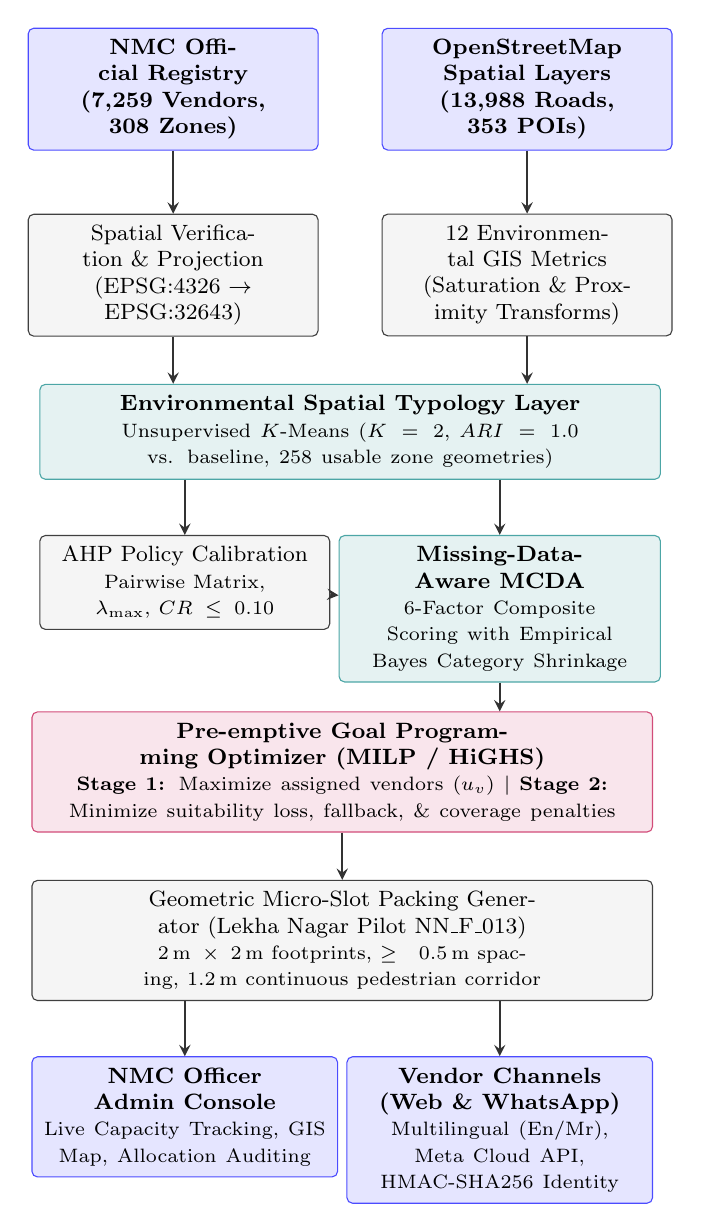
\begin{tikzpicture}[
    node distance=1.1cm and 1.2cm,
    box/.style={
        rectangle, draw=black!75, fill=gray!8, rounded corners=2pt,
        text centered, font=\footnotesize, minimum height=0.7cm, inner sep=4pt
    },
    primary/.style={
        box, fill=blue!10, draw=blue!70, font=\footnotesize\bfseries
    },
    accent/.style={
        box, fill=teal!10, draw=teal!70, font=\footnotesize\bfseries
    },
    opt/.style={
        box, fill=purple!10, draw=purple!70, font=\footnotesize\bfseries
    },
    layer/.style={
        rectangle, draw=black!40, dashed, rounded corners=4pt, inner sep=6pt, fill=black!2
    },
    arrow/.style={
        ->, >=stealth, thick, draw=black!80
    }
]

% Top Layer: Data Ingestion
\node[primary, text width=3.4cm] (nmc_data) {NMC Official Registry\\(7,259 Vendors, 308 Zones)};
\node[primary, text width=3.4cm, right=0.8cm of nmc_data] (osm_data) {OpenStreetMap Spatial Layers\\(13,988 Roads, 353 POIs)};

% Layer 2: Spatial Feature Engineering & Clustering
\node[box, text width=3.4cm, below=0.8cm of nmc_data] (geom_prep) {Spatial Verification \& Projection\\(EPSG:4326 $\to$ EPSG:32643)};
\node[box, text width=3.4cm, below=0.8cm of osm_data] (gis_feat) {12 Environmental GIS Metrics\\(Saturation \& Proximity Transforms)};

\node[accent, text width=7.6cm, below=0.6cm of $(geom_prep.south)!0.5!(gis_feat.south)$] (kmeans) {
    Environmental Spatial Typology Layer\\
    \normalfont{\scriptsize Unsupervised $K$-Means ($K=2$, $ARI=1.0$ vs. baseline, 258 usable zone geometries)}
};

% Layer 3: Decision Engine
\node[box, text width=3.4cm, below=0.7cm of kmeans.south west, anchor=north west] (ahp_engine) {
    AHP Policy Calibration\\
    \normalfont{\scriptsize Pairwise Matrix, $\lambda_{\max}$, $CR \le 0.10$}
};
\node[accent, text width=3.8cm, below=0.7cm of kmeans.south east, anchor=north east] (mcda_engine) {
    Missing-Data-Aware MCDA\\
    \normalfont{\scriptsize 6-Factor Composite Scoring with Empirical Bayes Category Shrinkage}
};

% Layer 4: Mathematical Optimization & Micro-Allocation
\node[opt, text width=7.6cm, below=0.7cm of $(ahp_engine.south)!0.5!(mcda_engine.south)$] (milp) {
    Pre-emptive Goal Programming Optimizer (MILP / HiGHS)\\
    \normalfont{\scriptsize \textbf{Stage 1:} Maximize assigned vendors ($u_v$) $\mid$ \textbf{Stage 2:} Minimize suitability loss, fallback, \& coverage penalties}
};

\node[box, text width=7.6cm, below=0.6cm of milp] (micro_alloc) {
    Geometric Micro-Slot Packing Generator (Lekha Nagar Pilot NN\_F\_013)\\
    \normalfont{\scriptsize $2\,\text{m}\times 2\,\text{m}$ footprints, $\ge 0.5\,\text{m}$ spacing, $1.2\,\text{m}$ continuous pedestrian corridor}
};

% Layer 5: Operational Delivery & Interfaces
\node[primary, text width=3.6cm, below=0.7cm of micro_alloc.south west, anchor=north west] (admin_ui) {
    NMC Officer Admin Console\\
    \normalfont{\scriptsize Live Capacity Tracking, GIS Map, Allocation Auditing}
};
\node[primary, text width=3.6cm, below=0.7cm of micro_alloc.south east, anchor=north east] (vendor_channel) {
    Vendor Channels (Web \& WhatsApp)\\
    \normalfont{\scriptsize Multilingual (En/Mr), Meta Cloud API, HMAC-SHA256 Identity}
};

% Arrows
\draw[arrow] (nmc_data) -- (geom_prep);
\draw[arrow] (osm_data) -- (gis_feat);
\draw[arrow] (geom_prep) -- (kmeans.north -| geom_prep);
\draw[arrow] (gis_feat) -- (kmeans.north -| gis_feat);

\draw[arrow] (kmeans.south -| ahp_engine) -- (ahp_engine);
\draw[arrow] (ahp_engine) -- (mcda_engine);
\draw[arrow] (kmeans.south -| mcda_engine) -- (mcda_engine);

\draw[arrow] (mcda_engine) -- (milp.north -| mcda_engine);
\draw[arrow] (milp) -- (micro_alloc);

\draw[arrow] (micro_alloc.south -| admin_ui) -- (admin_ui);
\draw[arrow] (micro_alloc.south -| vendor_channel) -- (vendor_channel);

\end{tikzpicture}

    \caption{Multi-tier system architecture of VendorMap, detailing spatial ingestion, environmental typology, AHP-calibrated MCDA, pre-emptive Goal Programming, and multichannel delivery.}
    \label{fig:sys_architecture}
\end{figure*}

\section{Flowchart}
\label{sec:flowchart}

Fig.~\ref{fig:sys_workflow} illustrates the end-to-end operational flowchart of the VendorMap relocation and allocation workflow, detailing statutory eligibility gating, capacity verification, and fallback handling.

\begin{figure}[htbp]
    \centering
    % End-to-End Workflow Diagram in TikZ
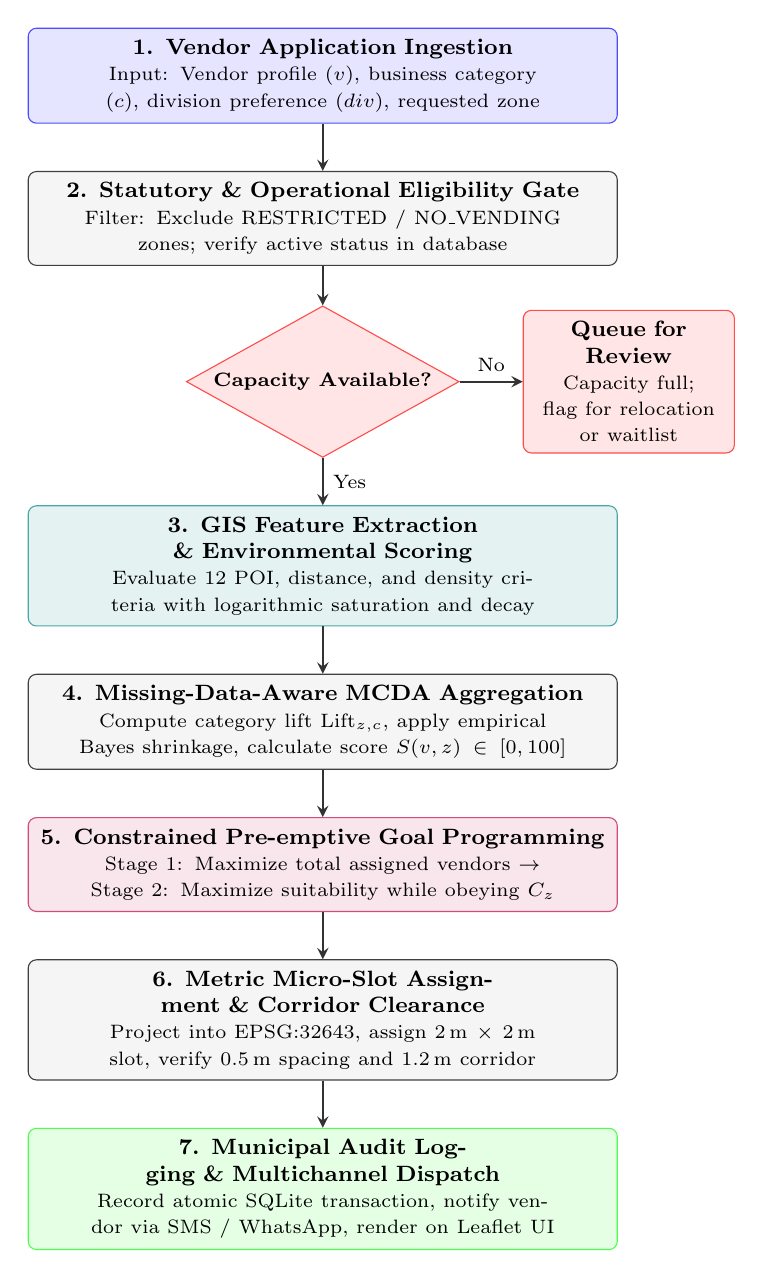
\begin{tikzpicture}[
    node distance=0.8cm,
    stepbox/.style={
        rectangle, draw=black!75, fill=gray!8, rounded corners=3pt,
        text centered, font=\footnotesize, minimum height=0.65cm, inner sep=4pt
    },
    decision/.style={
        diamond, draw=red!70, fill=red!10, text centered, font=\scriptsize\bfseries,
        inner sep=1.5pt, aspect=1.8
    },
    arrow/.style={
        ->, >=stealth, thick, draw=black!80
    }
]

% Steps
\node[stepbox, text width=7.2cm, fill=blue!10, draw=blue!70] (step1) {
    \textbf{1. Vendor Application Ingestion}\\
    \scriptsize Input: Vendor profile ($v$), business category ($c$), division preference ($div$), requested zone
};

\node[stepbox, text width=7.2cm, below=0.6cm of step1] (step2) {
    \textbf{2. Statutory \& Operational Eligibility Gate}\\
    \scriptsize Filter: Exclude RESTRICTED / NO\_VENDING zones; verify active status in database
};

\node[decision, below=0.5cm of step2] (dec1) {Capacity Available?};

\node[stepbox, text width=7.2cm, below=0.6cm of dec1, fill=teal!10, draw=teal!70] (step3) {
    \textbf{3. GIS Feature Extraction \& Environmental Scoring}\\
    \scriptsize Evaluate 12 POI, distance, and density criteria with logarithmic saturation and decay
};

\node[stepbox, text width=7.2cm, below=0.6cm of step3] (step4) {
    \textbf{4. Missing-Data-Aware MCDA Aggregation}\\
    \scriptsize Compute category lift $\text{Lift}_{z,c}$, apply empirical Bayes shrinkage, calculate score $S(v,z) \in [0, 100]$
};

\node[stepbox, text width=7.2cm, below=0.6cm of step4, fill=purple!10, draw=purple!70] (step5) {
    \textbf{5. Constrained Pre-emptive Goal Programming}\\
    \scriptsize Stage 1: Maximize total assigned vendors $\to$ Stage 2: Maximize suitability while obeying $C_z$
};

\node[stepbox, text width=7.2cm, below=0.6cm of step5] (step6) {
    \textbf{6. Metric Micro-Slot Assignment \& Corridor Clearance}\\
    \scriptsize Project into EPSG:32643, assign $2\,\text{m}\times 2\,\text{m}$ slot, verify $0.5\,\text{m}$ spacing and $1.2\,\text{m}$ corridor
};

\node[stepbox, text width=7.2cm, below=0.6cm of step6, fill=green!10, draw=green!70] (step7) {
    \textbf{7. Municipal Audit Logging \& Multichannel Dispatch}\\
    \scriptsize Record atomic SQLite transaction, notify vendor via SMS / WhatsApp, render on Leaflet UI
};

% Failure Node
\node[stepbox, text width=2.4cm, fill=red!10, draw=red!70, right=0.8cm of dec1] (reject) {
    \textbf{Queue for Review}\\
    \scriptsize Capacity full; flag for relocation or waitlist
};

% Connectors
\draw[arrow] (step1) -- (step2);
\draw[arrow] (step2) -- (dec1);
\draw[arrow] (dec1) -- node[right, font=\scriptsize] {Yes} (step3);
\draw[arrow] (dec1) -- node[above, font=\scriptsize] {No} (reject);
\draw[arrow] (step3) -- (step4);
\draw[arrow] (step4) -- (step5);
\draw[arrow] (step5) -- (step6);
\draw[arrow] (step6) -- (step7);

\end{tikzpicture}

    \caption{End-to-end operational flowchart of the VendorMap vendor relocation and micro-slot allocation workflow.}
    \label{fig:sys_workflow}
\end{figure}

\section{Algorithm}
\label{sec:algorithm}

Algorithm~\ref{alg:vendormap_pipeline} formalizes the complete computational execution sequence of the VendorMap allocation engine.

\begin{algorithm}[htbp]
\caption{End-to-End VendorMap Relocation and Micro-Allocation Pipeline}
\label{alg:vendormap_pipeline}
\begin{algorithmic}[1]
\Require Vendor relocation demand batch $\mathcal{V}_{\text{req}}$, Municipal zone registry $\mathcal{Z}$, Spatial GIS layers $\mathbf{X}_{\text{GIS}}$
\Ensure Optimal binary allocation matrix $\mathbf{X}^*$ and physical metric slot polygons $\mathcal{S}$
\State Identify eligible candidate zones: $\mathcal{Z}_{\text{elig}} \gets \{z \in \mathcal{Z} \mid \text{Type}_z = \text{FREE} \land C_z - \text{ActiveCount}_z > 0\}$
\For{each vendor $v \in \mathcal{V}_{\text{req}}$}
    \State Extract business category $c_v$ and preferred division $d_v$
    \For{each zone $z \in \mathcal{Z}_{\text{elig}}$}
        \State Compute leave-group-out category lift $\text{Lift}_{z,c_v}$ and reliability $R(n_z)$ (Eq.~\ref{eq:shrinkage_form}--\ref{eq:fbus_form})
        \State Compute non-linear feature scores $f_{\text{com}}, f_{\text{acc}}, f_{\text{fac}}, f_{\text{pref}}, f_{\text{hist}}$ (Eq.~\ref{eq:sat_transform}--\ref{eq:prox_transform})
        \State Compute normalized suitability score $\text{Score}(v,z)$ and coverage $\text{Coverage}(v,z)$ (Eq.~\ref{eq:mcda_norm_form})
    \EndFor
\EndFor
\State \textbf{// Stage 1: Solve Cardinality MILP via HiGHS Solver}
\State $U^* \gets \min_{\mathbf{x}, \mathbf{u}} \sum_{v \in \mathcal{V}_{\text{req}}} u_v$ subject to single assignment and live capacity constraints
\State \textbf{// Stage 2: Solve Lexicographic Quality MILP}
\State $\mathbf{X}^* \gets \arg\min_{\mathbf{x}} \sum_{v,z} x_{v,z} \Psi(v, z)$ subject to capacity constraints and $\sum_v u_v = U^*$
\For{each assigned zone $z$ with boundary polygon $\Omega_z$}
    \State Project $\Omega_z$ into metric coordinates (EPSG:32643 / UTM Zone 43N)
    \State Determine dominant alignment angle $\theta^* = \arg\max \text{Length}(\text{Edge}(\text{MinRotatedRect}(\Omega_z)))$
    \State Pack $2.0\,\text{m} \times 2.0\,\text{m}$ slots maintaining $\ge 0.5\,\text{m}$ inter-slot clearance
    \State Reserve continuous $1.2\,\text{m}$ pedestrian clearance corridor
    \State Transform validated slot polygons $\mathcal{S}_z$ back to EPSG:4326 for Leaflet map rendering
\EndFor
\State \Return $\mathbf{X}^*$ and $\mathcal{S}$
\end{algorithmic}
\end{algorithm}


% Chapter 4: Project Requirement Specifications
% ==============================================================================
% Chapter 4: Project Requirement Specifications
% ==============================================================================
\chapter{Project Requirement Specifications}
\label{ch:requirements}

This chapter provides a detailed specification of the hardware, software, functional, and non-functional requirements governing the implementation and deployment of VendorMap, alongside critical operational constraints and domain assumptions.

\section{Hardware Requirements}
\label{sec:hardware_requirements}

The system architecture is engineered to run cost-effectively across standard municipal workstation hardware and commodity cloud servers, while enabling low-resource vendor mobile devices to access platform services.

\subsection{Development and Municipal Server Environment}
\begin{itemize}
    \item \textbf{Processor:} Modern x86\_64 multi-core processor (Intel Core i5 / i7 8th Gen or AMD Ryzen 5 / 7, $\ge 4$ physical cores, $2.4\,\text{GHz}$ base clock).
    \item \textbf{System Memory (RAM):} Minimum 8 GB DDR4 RAM (16 GB recommended for concurrent GIS vector layer manipulation, spatial clustering, and MILP optimization).
    \item \textbf{Storage:} Minimum 256 GB Solid State Drive (NVMe SSD preferred) to support high-throughput SQLite Write-Ahead Logging (WAL) and spatial GeoPackage I/O.
    \item \textbf{Network Interface:} Gigabit Ethernet / High-speed Wi-Fi network interface for live Meta WhatsApp Cloud API webhook communication and OpenStreetMap tile streaming.
\end{itemize}

\subsection{End-User Client Devices (Town-Planning Officers \& Street Vendors)}
\begin{itemize}
    \item \textbf{Officer Admin Desktop / Laptop:} Any standard desktop or laptop PC capable of running a modern Chromium-based web browser with WebGL support for interactive React-Leaflet GIS maps.
    \item \textbf{Vendor Mobile Device (Web Portal):} Any smartphone running Android 8.0+ or iOS 12.0+ with modern browser support (Chrome, Safari, Firefox), minimum 2 GB RAM, and integrated GPS / A-GPS hardware.
    \item \textbf{Vendor Mobile Device (Conversational WhatsApp):} Any basic smartphone or smart feature phone supporting WhatsApp Messenger with standard 2G/3G/4G/5G mobile cellular connectivity.
\end{itemize}

\section{Software Requirements}
\label{sec:software_requirements}

The software stack utilizes production-grade, open-source frameworks and libraries ensuring zero software licensing overhead for municipal deployment:

\subsection{Backend Development and Runtime Environment}
\begin{itemize}
    \item \textbf{Operating System:} Microsoft Windows 11 / 10 (64-bit) or Ubuntu Linux 22.04 LTS.
    \item \textbf{Core Language Runtime:} Python 3.10.12 (managed via isolated virtual environments).
    \item \textbf{ASGI Web Framework:} FastAPI 0.141.1 with Uvicorn 0.54.0 ASGI server and Pydantic v2 data contract validation.
    \item \textbf{Persistence Layer:} SQLite 3.39+ with Write-Ahead Logging (WAL) and SQLAlchemy 2.1 Core query abstraction.
    \item \textbf{Scientific and Spatial Computing:} NumPy 2.5, Pandas 3.0, SciPy 1.18, Scikit-learn 1.9, Shapely 2.1 (computational geometry), and PyProj 3.8 (cartographic transformations).
    \item \textbf{Mathematical Optimization:} HiGHS MILP Solver~\cite{huang2023highs} integrated natively into \texttt{scipy.optimize.milp}.
    \item \textbf{Cryptographic Security:} Python \texttt{hmac} and \texttt{hashlib} libraries enforcing HMAC-SHA256 identity obfuscation.
    \item \textbf{External Integration:} Official Meta WhatsApp Cloud API (Graph API v21.0+) via asynchronous HTTP client (\texttt{httpx}).
\end{itemize}

\subsection{Frontend Development and User Interface Stack}
\begin{itemize}
    \item \textbf{Runtime Environment:} Node.js v18.19.0 LTS and npm 9.x / 10.x package manager.
    \item \textbf{Build Tool \& Bundler:} Vite 5.x for hot-module replacement and optimized ES module bundling.
    \item \textbf{UI Framework:} React 18.2 with functional component architecture and custom React hooks.
    \item \textbf{Geospatial Visualization:} Leaflet 1.9 with React-Leaflet 4.2 for vector polygon rendering, custom tile caching, and real-time GPS geolocation watching.
    \item \textbf{Styling and Design System:} Clean Vanilla CSS design system utilizing CSS Custom Properties (Tokens) for high-performance rendering without third-party utility bloat.
    \item \textbf{Internationalization (i18n):} Custom multilingual context provider supporting real-time switching between English (\texttt{en}) and Marathi (\texttt{mr}).
\end{itemize}

\section{Functional Requirements}
\label{sec:functional_requirements}

Table~\ref{tab:functional_requirements} summarizes the core functional requirements implemented in VendorMap, categorized by functional module.

\begin{table*}[htbp]
\caption{Detailed Functional Requirements Matrix}
\label{tab:functional_requirements}
\centering
\small
\begin{tabularx}{\textwidth}{lp{0.22\textwidth}X}
\toprule
\textbf{Req. ID} & \textbf{Module} & \textbf{Functional Requirement Description} \\
\midrule
\textbf{FR-01} & Authentication & The system shall authenticate vendors via mobile phone OTP verification without storing plaintext phone numbers, utilizing HMAC-SHA256 identity hashing. \\
\textbf{FR-02} & Authentication & The system shall support secure administrative login for municipal town-planning officers using environment-configured credentials and HttpOnly session cookies. \\
\textbf{FR-03} & Vendor Onboarding & The system shall allow unverified vendors to complete a single verified operational profile including full name, business category, and division preference. \\
\textbf{FR-04} & Zone Registry & The system shall maintain an official registry of 308 municipal vending zones, tracking legal classification, official capacity, active occupants, and available quota. \\
\textbf{FR-05} & Recommendation & The system shall compute personalized zone suitability scores ($0$--$100$) for any vendor profile using 6-factor MCDA with empirical Bayes category shrinkage ($M=20.0$). \\
\textbf{FR-06} & Relocation Request & The system shall allow authenticated vendors to submit new zone allocation and relocation requests with automated validation against duplicate pending requests. \\
\textbf{FR-07} & Batch Optimization & The system shall execute two-stage pre-emptive Goal Programming (MILP via HiGHS) across batches of vendor requests, guaranteeing zero capacity over-allocation. \\
\textbf{FR-08} & Policy Calibration & The system shall provide officers with an interactive AHP pairwise matrix interface to calibrate factor weights, dynamically validating Consistency Ratio ($CR \le 0.10$). \\
\textbf{FR-09} & Micro-Slot Packing & The system shall pack $2\,\text{m} \times 2\,\text{m}$ vending stalls within zone boundary polygons in UTM Zone 43N projection, enforcing $\ge 0.5\,\text{m}$ spacing and $1.2\,\text{m}$ corridor clearance. \\
\textbf{FR-10} & Slot Management & The system shall allow officers to assign, block, or release individual micro-slots with atomic SQLite transaction isolation, preventing concurrent double-booking. \\
\textbf{FR-11} & Pedestrian Navigation & The system shall provide approved vendors with single-map turn-by-turn walking directions directly from their live GPS location to their assigned micro-slot. \\
\textbf{FR-12} & WhatsApp Conversational & The system shall support direct Meta WhatsApp Cloud API webhooks with HMAC signature verification, message deduplication, and a multi-turn bilingual state machine. \\
\textbf{FR-13} & Audit Trail & The system shall log all administrative actions, status transitions, and slot assignments into an immutable SQLite audit log table for civic accountability. \\
\bottomrule
\end{tabularx}
\end{table*}

\section{Non-Functional Requirements}
\label{sec:non_functional_requirements}

\begin{enumerate}
    \item \textbf{Performance and Response Latency:}
    \begin{itemize}
        \item Single-vendor MCDA suitability calculation across all 308 municipal zones shall execute in under $150\,\text{milliseconds}$.
        \item Batch Goal Programming optimization for batches up to 100 vendors shall converge to global optimality in under $2.0\,\text{seconds}$.
        \item Micro-slot geometric packing generation for boundary polygons shall execute in under $500\,\text{milliseconds}$.
        \item Interactive Leaflet map panning, zooming, and polygon rendering shall maintain $\ge 60\,\text{frames per second}$ on standard client hardware.
    \end{itemize}
    
    \item \textbf{Data Privacy and Cryptographic Minimization:}
    \begin{itemize}
        \item Sensitive Personally Identifiable Information (PII)---specifically vendor telephone numbers and alternate mobile numbers---shall never be stored in plaintext within database tables, server log files, or error dumps.
        \item Phone numbers shall be normalized to E.164 format and hashed via HMAC-SHA256 using an institutional secret key (\texttt{AUTH\_HMAC\_SECRET}).
        \item Active session tokens shall be stored in browser cookies configured with \texttt{HttpOnly}, \texttt{SameSite=Lax}, and conditional production \texttt{Secure} flags.
    \end{itemize}
    
    \item \textbf{Reliability and Transactional Integrity:}
    \begin{itemize}
        \item All critical state transitions (such as slot status updates, request approvals, and capacity decrements) shall execute within atomic SQLite database transactions with immediate locking.
        \item Inbound Meta WhatsApp webhook notifications shall enforce idempotent message deduplication using unique Meta \texttt{message\_id} indices.
    \end{itemize}
    
    \item \textbf{Usability and Accessibility:}
    \begin{itemize}
        \item The vendor user interface shall be fully internationalized, providing instantaneous language switching between English and Marathi.
        \item Design tokens shall maintain high contrast ratios ($> 4.5:1$) conforming to WCAG 2.1 AA accessibility guidelines.
    \end{itemize}
\end{enumerate}

\section{System Constraints and Assumptions}
\label{sec:constraints_assumptions}

\subsection{System Constraints}
\begin{enumerate}
    \item \textbf{Statutory Regulatory Boundaries:} The system cannot create or dissolve vending zones independently of the official gazetted records of the Nashik Municipal Corporation and Town Vending Committee.
    \item \textbf{Cartographic Survey Availability:} Of the 308 official zones, 258 possess verified usable spatial reference geometries. The remaining 50 zones lack digitized polygon coordinates and are formally flagged for municipal physical re-survey.
    \item \textbf{Client GPS Accuracy Constraints:} In dense urban canyon environments or beneath dense tree canopies, mobile GPS accuracy may degrade to $\pm 15$--$30\,\text{meters}$. The navigation interface explicitly labels final approach guidance as approximate.
    \item \textbf{Single Active Allocation Rule:} A registered vendor is legally permitted to hold at most one active municipal zone allocation and one physical micro-slot at any given time.
\end{enumerate}

\subsection{Domain Assumptions}
\begin{enumerate}
    \item \textbf{Zone Capacity Legitimacy:} Official zone capacities ($C_z$) documented in the NMC municipal gazette are assumed to reflect legally deliberated Town Vending Committee limits.
    \item \textbf{Spatial OpenStreetMap Coverage:} Road geometries, pedestrian footways, and commercial POIs extracted from OpenStreetMap are assumed to provide a representative proxy for urban commercial vibrancy.
    \item \textbf{Vendor Mobile Access:} It is assumed that street vendors or a designated family member possess basic smartphone access with SMS receiving capability or WhatsApp messaging functionality.
\end{enumerate}


% Chapter 5: High-Level Design
% ==============================================================================
% Chapter 5: High-Level Design
% ==============================================================================
\chapter{High-Level Design}
\label{ch:high_level_design}

This chapter articulates the structural and behavioural design of VendorMap through formal architectural models, including the relational Entity-Relationship Diagram (ERD), Data Flow Diagrams (Level 0 and Level 1), and complete Unified Modeling Language (UML) specifications (Use Case, Service Class Architecture, Sequence, and Activity diagrams).

\section{Entity Relationship Diagram (ERD)}
\label{sec:erd}

The operational persistence layer is implemented in SQLite using SQLAlchemy Core abstraction. The schema strictly decouples operational transaction management from research model artifacts. Fig.~\ref{fig:erd_diagram} depicts the Entity-Relationship Diagram modeling the core database entities, primary/foreign key relationships, and structural cardinality.

\begin{figure*}[htbp]
\centering
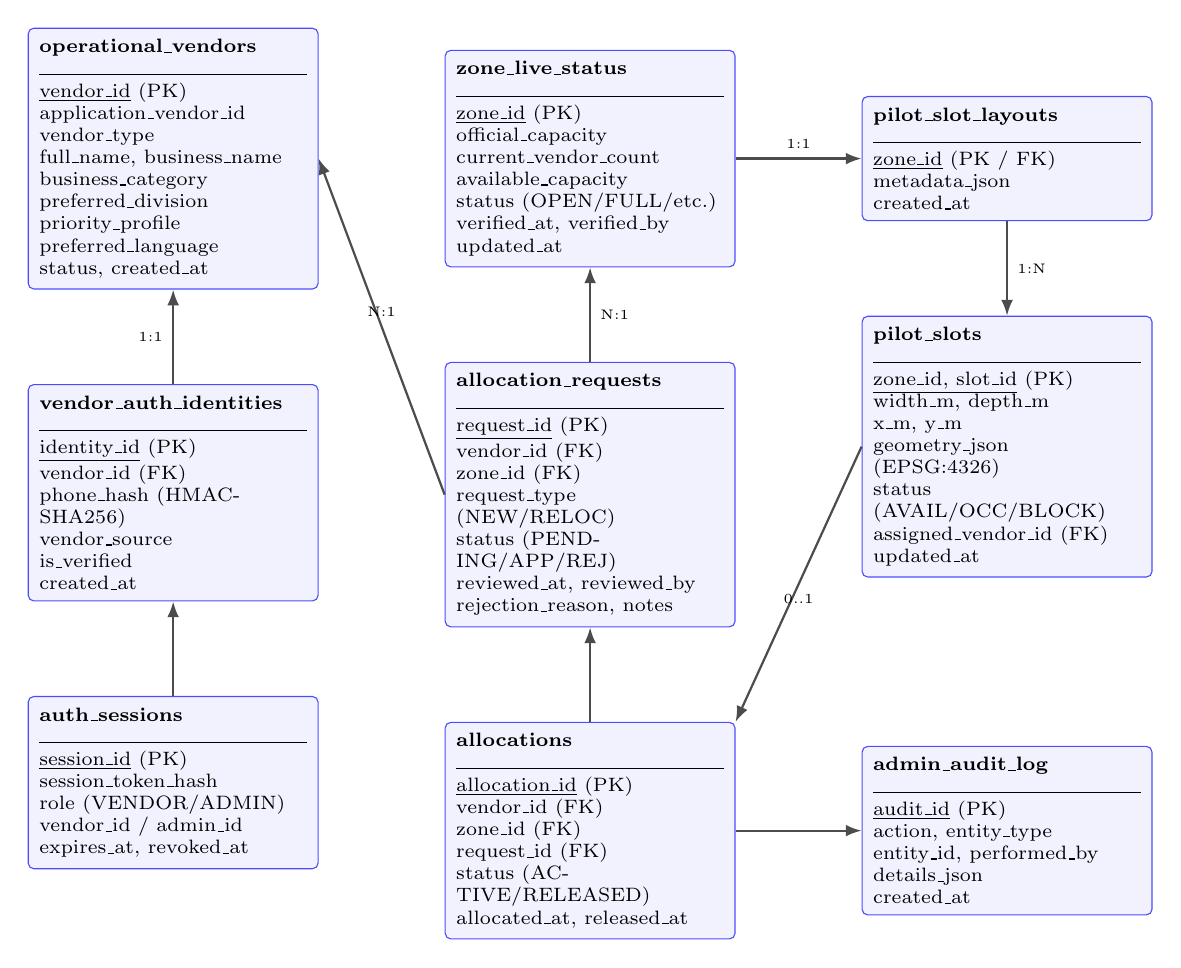
\begin{tikzpicture}[
    node distance=1.6cm and 1.8cm,
    entity/.style={
        rectangle, draw=blue!70, fill=blue!5, rounded corners=2pt,
        font=\scriptsize, inner sep=4pt, text width=3.4cm
    },
    header/.style={
        font=\scriptsize\bfseries, fill=blue!15, text centered, draw=blue!70
    },
    rel/.style={
        draw=black!70, thick, -{Latex[length=2mm]}
    },
    carrow/.style={
        draw=black!75, thick
    }
]

% Operational Entities
\node[entity] (vendor) {
    \textbf{operational\_vendors}\\
    \hrulefill\\
    \underline{vendor\_id} (PK)\\
    application\_vendor\_id\\
    vendor\_type\\
    full\_name, business\_name\\
    business\_category\\
    preferred\_division\\
    priority\_profile\\
    preferred\_language\\
    status, created\_at
};

\node[entity, right=1.6cm of vendor] (zone) {
    \textbf{zone\_live\_status}\\
    \hrulefill\\
    \underline{zone\_id} (PK)\\
    official\_capacity\\
    current\_vendor\_count\\
    available\_capacity\\
    status (OPEN/FULL/etc.)\\
    verified\_at, verified\_by\\
    updated\_at
};

\node[entity, below=1.2cm of vendor] (auth_ident) {
    \textbf{vendor\_auth\_identities}\\
    \hrulefill\\
    \underline{identity\_id} (PK)\\
    vendor\_id (FK)\\
    phone\_hash (HMAC-SHA256)\\
    vendor\_source\\
    is\_verified\\
    created\_at
};

\node[entity, below=1.2cm of zone] (alloc_req) {
    \textbf{allocation\_requests}\\
    \hrulefill\\
    \underline{request\_id} (PK)\\
    vendor\_id (FK)\\
    zone\_id (FK)\\
    request\_type (NEW/RELOC)\\
    status (PENDING/APP/REJ)\\
    reviewed\_at, reviewed\_by\\
    rejection\_reason, notes
};

\node[entity, below=1.2cm of alloc_req] (alloc) {
    \textbf{allocations}\\
    \hrulefill\\
    \underline{allocation\_id} (PK)\\
    vendor\_id (FK)\\
    zone\_id (FK)\\
    request\_id (FK)\\
    status (ACTIVE/RELEASED)\\
    allocated\_at, released\_at
};

\node[entity, right=1.6cm of zone] (pilot_layout) {
    \textbf{pilot\_slot\_layouts}\\
    \hrulefill\\
    \underline{zone\_id} (PK / FK)\\
    metadata\_json\\
    created\_at
};

\node[entity, below=1.2cm of pilot_layout] (pilot_slot) {
    \textbf{pilot\_slots}\\
    \hrulefill\\
    \underline{zone\_id, slot\_id} (PK)\\
    width\_m, depth\_m\\
    x\_m, y\_m\\
    geometry\_json (EPSG:4326)\\
    status (AVAIL/OCC/BLOCK)\\
    assigned\_vendor\_id (FK)\\
    updated\_at
};

\node[entity, below=1.2cm of auth_ident] (sessions) {
    \textbf{auth\_sessions}\\
    \hrulefill\\
    \underline{session\_id} (PK)\\
    session\_token\_hash\\
    role (VENDOR/ADMIN)\\
    vendor\_id / admin\_id\\
    expires\_at, revoked\_at
};

\node[entity, right=1.6cm of alloc] (audit) {
    \textbf{admin\_audit\_log}\\
    \hrulefill\\
    \underline{audit\_id} (PK)\\
    action, entity\_type\\
    entity\_id, performed\_by\\
    details\_json\\
    created\_at
};

% Connectors
\draw[rel] (auth_ident.north) -- node[left, font=\tiny] {1:1} (vendor.south);
\draw[rel] (sessions.north) -- (auth_ident.south);
\draw[rel] (alloc_req.west) -- node[above, font=\tiny] {N:1} (vendor.east);
\draw[rel] (alloc_req.north) -- node[right, font=\tiny] {N:1} (zone.south);
\draw[rel] (alloc.north) -- (alloc_req.south);
\draw[rel] (pilot_layout.south) -- node[right, font=\tiny] {1:N} (pilot_slot.north);
\draw[rel] (zone.east) -- node[above, font=\tiny] {1:1} (pilot_layout.west);
\draw[rel] (alloc.east) -- (audit.west);
\draw[rel] (pilot_slot.west) -- node[below, font=\tiny] {0..1} (alloc.north east);

\end{tikzpicture}
\caption{Entity-Relationship Diagram (ERD) of the VendorMap operational database schema.}
\label{fig:erd_diagram}
\end{figure*}

\section{Data Flow Diagrams (DFD)}
\label{sec:dfd}

\subsection{Level 0 DFD (Context Diagram)}
Fig.~\ref{fig:dfd_level0} illustrates the Level 0 Context Diagram of VendorMap, depicting the external entities interacting across system boundaries.

\begin{figure}[htbp]
\centering
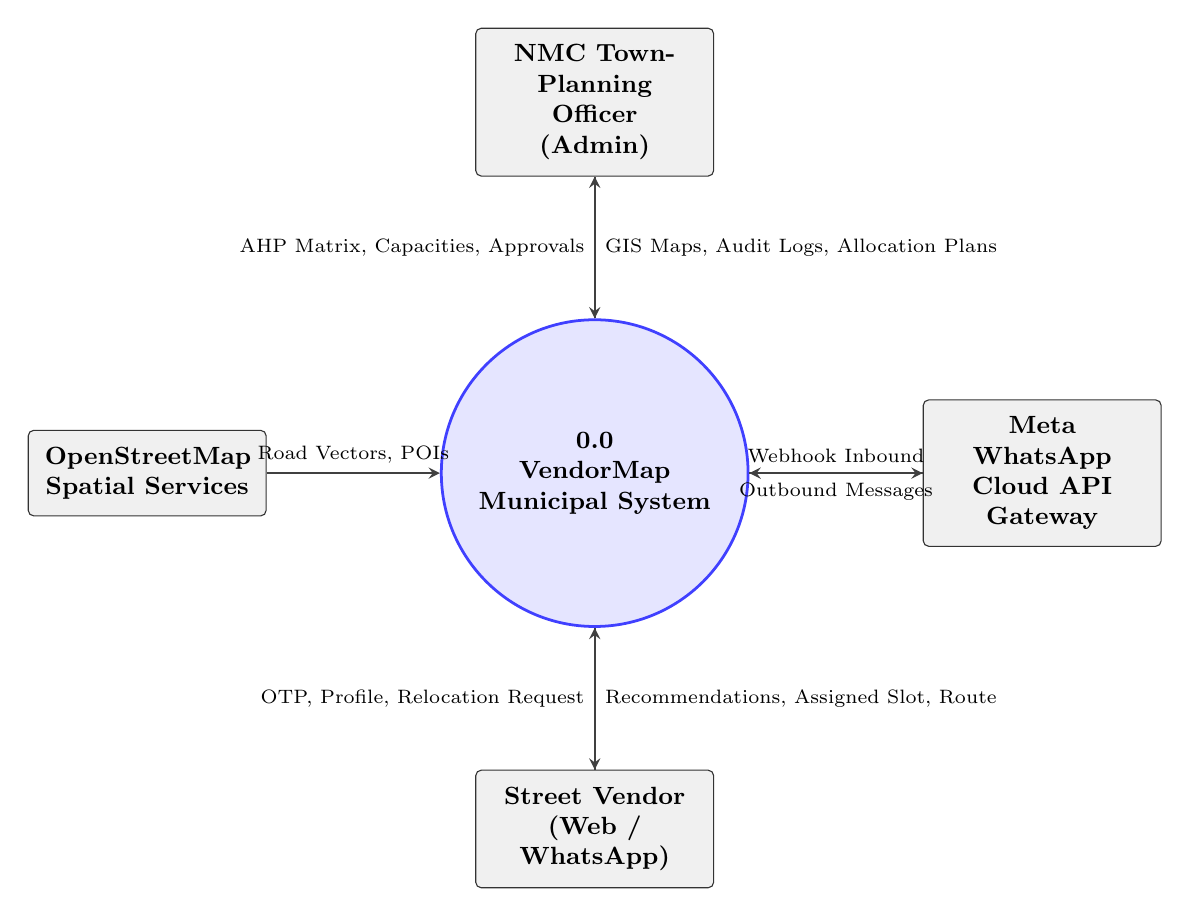
\begin{tikzpicture}[
    node distance=2.2cm,
    ext/.style={
        rectangle, draw=black!80, fill=gray!12, rounded corners=2pt,
        font=\small\bfseries, text centered, inner sep=6pt, text width=2.6cm
    },
    proc/.style={
        circle, draw=blue!75, fill=blue!10, line width=1pt,
        font=\small\bfseries, text centered, inner sep=6pt, text width=3.2cm
    },
    arrow/.style={
        ->, >=stealth, thick, draw=black!75
    }
]

\node[proc] (system) {0.0\\VendorMap\\Municipal System};

\node[ext, above=1.8cm of system] (officer) {NMC Town-Planning\\Officer (Admin)};
\node[ext, below=1.8cm of system] (vendor) {Street Vendor\\(Web / WhatsApp)};
\node[ext, left=2.2cm of system] (osm) {OpenStreetMap\\Spatial Services};
\node[ext, right=2.2cm of system] (meta) {Meta WhatsApp\\Cloud API Gateway};

\draw[arrow] (officer) -- node[left, font=\scriptsize] {AHP Matrix, Capacities, Approvals} (system);
\draw[arrow] (system) -- node[right, font=\scriptsize] {GIS Maps, Audit Logs, Allocation Plans} (officer);

\draw[arrow] (vendor) -- node[left, font=\scriptsize] {OTP, Profile, Relocation Request} (system);
\draw[arrow] (system) -- node[right, font=\scriptsize] {Recommendations, Assigned Slot, Route} (vendor);

\draw[arrow] (osm) -- node[above, font=\scriptsize] {Road Vectors, POIs} (system);
\draw[arrow] (meta) -- node[above, font=\scriptsize] {Webhook Inbound} (system);
\draw[arrow] (system) -- node[below, font=\scriptsize] {Outbound Messages} (meta);

\end{tikzpicture}
\caption{Level 0 Context Data Flow Diagram (DFD) of VendorMap.}
\label{fig:dfd_level0}
\end{figure}

\subsection{Level 1 DFD (Decomposed Processes)}
Fig.~\ref{fig:dfd_level1} decomposes the system into six core operational processes and five internal data repositories.

\begin{figure*}[htbp]
\centering
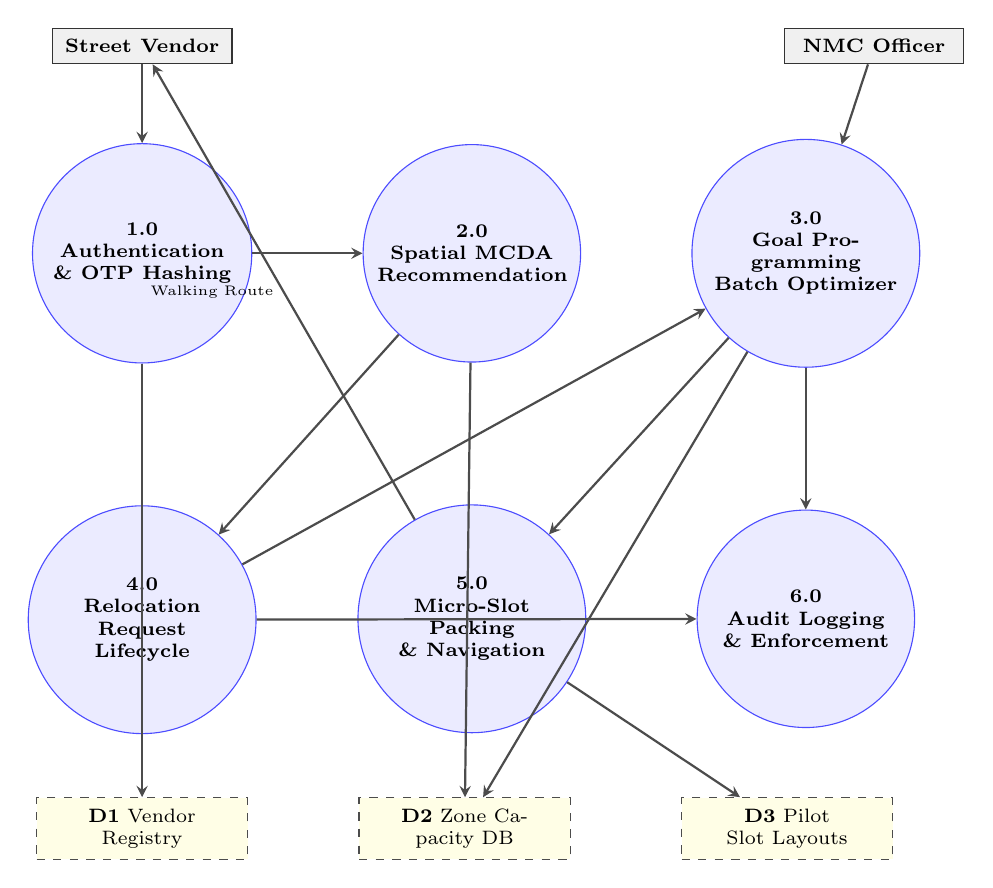
\begin{tikzpicture}[
    node distance=1.4cm and 1.4cm,
    proc/.style={
        circle, draw=blue!70, fill=blue!8,
        font=\scriptsize\bfseries, text centered, inner sep=3pt, text width=2.4cm
    },
    store/.style={
        rectangle, draw=black!70, fill=yellow!10, dashed,
        font=\scriptsize, inner sep=4pt, text width=2.4cm, text centered
    },
    ext/.style={
        rectangle, draw=black!80, fill=gray!12,
        font=\scriptsize\bfseries, text centered, inner sep=4pt, text width=2.0cm
    },
    arrow/.style={
        ->, >=stealth, thick, draw=black!70
    }
]

% External entities
\node[ext] (ext_vendor) {Street Vendor};
\node[ext, right=7.0cm of ext_vendor] (ext_admin) {NMC Officer};

% Processes
\node[proc, below=1.0cm of ext_vendor] (p1) {1.0\\Authentication\\\& OTP Hashing};
\node[proc, right=1.4cm of p1] (p2) {2.0\\Spatial MCDA\\Recommendation};
\node[proc, right=1.4cm of p2] (p3) {3.0\\Goal Programming\\Batch Optimizer};
\node[proc, below=1.8cm of p1] (p4) {4.0\\Relocation Request\\Lifecycle};
\node[proc, below=1.8cm of p2] (p5) {5.0\\Micro-Slot Packing\\\& Navigation};
\node[proc, below=1.8cm of p3] (p6) {6.0\\Audit Logging\\\& Enforcement};

% Data stores
\node[store, below=0.8cm of p4] (d1) {\textbf{D1} Vendor Registry};
\node[store, right=1.4cm of d1] (d2) {\textbf{D2} Zone Capacity DB};
\node[store, right=1.4cm of d2] (d3) {\textbf{D3} Pilot Slot Layouts};

% Flows
\draw[arrow] (ext_vendor) -- (p1);
\draw[arrow] (p1) -- (d1);
\draw[arrow] (p1) -- (p2);
\draw[arrow] (p2) -- (d2);
\draw[arrow] (p2) -- (p4);
\draw[arrow] (p4) -- (p3);
\draw[arrow] (ext_admin) -- (p3);
\draw[arrow] (p3) -- (d2);
\draw[arrow] (p3) -- (p5);
\draw[arrow] (p5) -- (d3);
\draw[arrow] (p5) -- node[left, font=\tiny] {Walking Route} (ext_vendor);
\draw[arrow] (p3) -- (p6);
\draw[arrow] (p4) -- (p6);

\end{tikzpicture}
\caption{Level 1 Data Flow Diagram (DFD) showing internal processes and operational stores.}
\label{fig:dfd_level1}
\end{figure*}

\section{UML Diagrams}
\label{sec:uml_diagrams}

\subsection{Use Case Diagram}
Fig.~\ref{fig:uml_usecase} details the system Use Case Diagram, categorizing actions available to Street Vendors, Town-Planning Officers, and the Meta WhatsApp Cloud API gateway.

\begin{figure}[htbp]
\centering
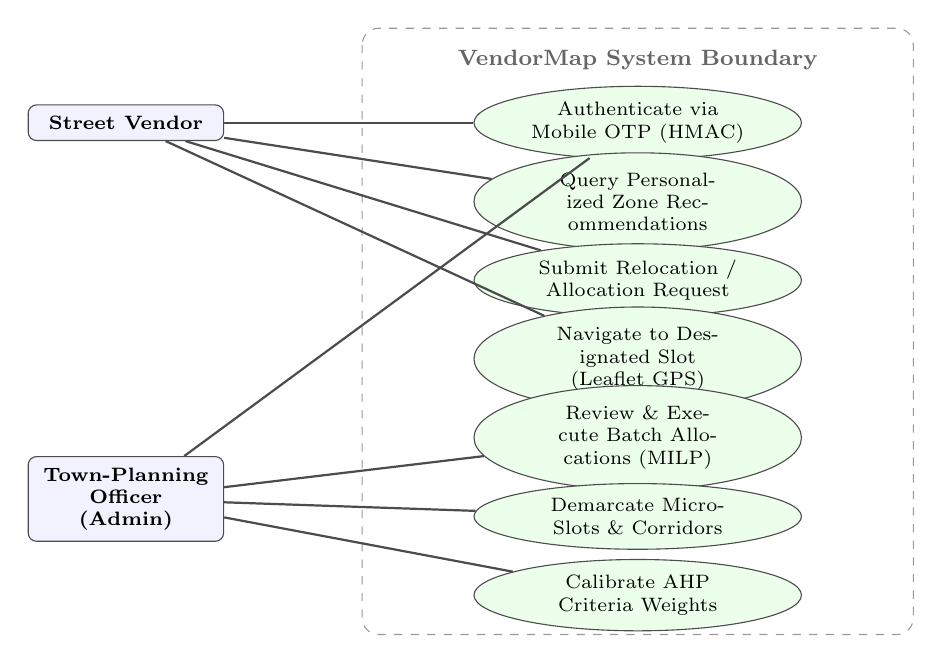
\begin{tikzpicture}[
    actor/.style={
        rectangle, draw=black!70, fill=blue!5, rounded corners=3pt,
        font=\scriptsize\bfseries, text centered, inner sep=4pt, text width=2.2cm
    },
    usecase/.style={
        ellipse, draw=black!70, fill=green!8,
        font=\scriptsize, text centered, inner sep=2pt, text width=2.8cm, minimum height=0.7cm
    },
    arrow/.style={
        -, thick, draw=black!70
    }
]

% Actors
\node[actor] (act_vendor) {Street Vendor};
\node[actor, below=4.0cm of act_vendor] (act_admin) {Town-Planning\\Officer (Admin)};

% Boundary box
\draw[dashed, black!40, rounded corners=6pt] (3.0, 1.2) rectangle (10.0, -6.5);
\node[font=\footnotesize\bfseries, color=black!60] at (6.5, 0.8) {VendorMap System Boundary};

% Use cases
\node[usecase] (uc1) at (6.5, 0.0) {Authenticate via Mobile OTP (HMAC)};
\node[usecase] (uc2) at (6.5, -1.0) {Query Personalized Zone Recommendations};
\node[usecase] (uc3) at (6.5, -2.0) {Submit Relocation / Allocation Request};
\node[usecase] (uc4) at (6.5, -3.0) {Navigate to Designated Slot (Leaflet GPS)};
\node[usecase] (uc5) at (6.5, -4.0) {Review \& Execute Batch Allocations (MILP)};
\node[usecase] (uc6) at (6.5, -5.0) {Demarcate Micro-Slots \& Corridors};
\node[usecase] (uc7) at (6.5, -6.0) {Calibrate AHP Criteria Weights};

% Connections
\draw[arrow] (act_vendor) -- (uc1);
\draw[arrow] (act_vendor) -- (uc2);
\draw[arrow] (act_vendor) -- (uc3);
\draw[arrow] (act_vendor) -- (uc4);

\draw[arrow] (act_admin) -- (uc1);
\draw[arrow] (act_admin) -- (uc5);
\draw[arrow] (act_admin) -- (uc6);
\draw[arrow] (act_admin) -- (uc7);

\end{tikzpicture}
\caption{UML Use Case Diagram representing primary actors and system capabilities.}
\label{fig:uml_usecase}
\end{figure}

\subsection{Service Architecture / Class Diagram}
VendorMap follows a service-oriented architectural pattern in Python. Fig.~\ref{fig:uml_class} illustrates the core domain services, repositories, and mathematical engines.

\begin{figure*}[htbp]
\centering
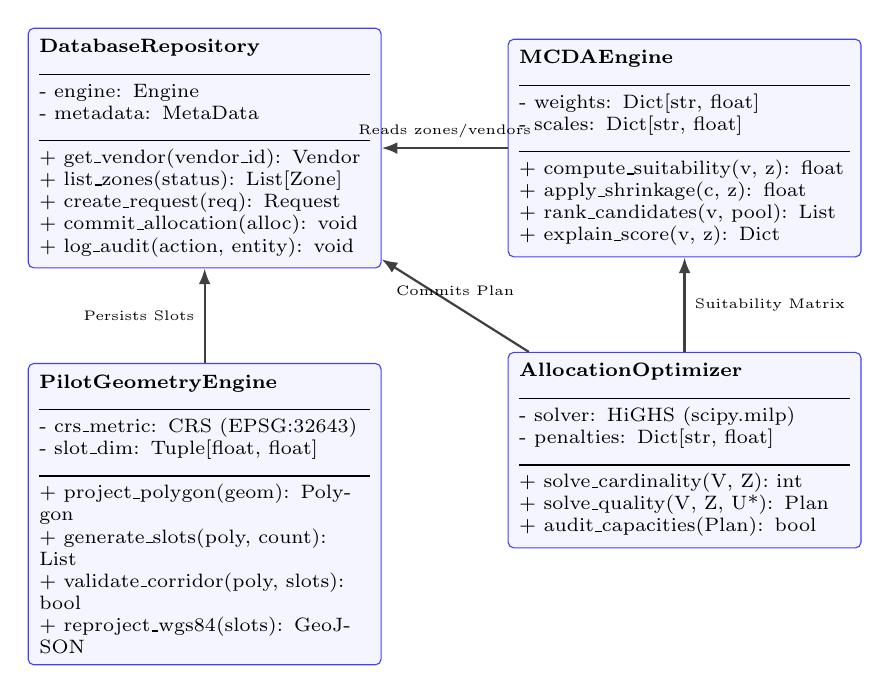
\begin{tikzpicture}[
    classbox/.style={
        rectangle, draw=blue!75, fill=blue!4, rounded corners=2pt,
        font=\scriptsize, inner sep=4pt, text width=4.2cm
    },
    arrow/.style={
        draw=black!75, thick, -{Latex[length=2mm]}
    }
]

\node[classbox] (repo) {
    \textbf{DatabaseRepository}\\
    \hrulefill\\
    - engine: Engine\\
    - metadata: MetaData\\
    \hrulefill\\
    + get\_vendor(vendor\_id): Vendor\\
    + list\_zones(status): List[Zone]\\
    + create\_request(req): Request\\
    + commit\_allocation(alloc): void\\
    + log\_audit(action, entity): void
};

\node[classbox, right=1.6cm of repo] (mcda) {
    \textbf{MCDAEngine}\\
    \hrulefill\\
    - weights: Dict[str, float]\\
    - scales: Dict[str, float]\\
    \hrulefill\\
    + compute\_suitability(v, z): float\\
    + apply\_shrinkage(c, z): float\\
    + rank\_candidates(v, pool): List\\
    + explain\_score(v, z): Dict
};

\node[classbox, below=1.2cm of repo] (geom) {
    \textbf{PilotGeometryEngine}\\
    \hrulefill\\
    - crs\_metric: CRS (EPSG:32643)\\
    - slot\_dim: Tuple[float, float]\\
    \hrulefill\\
    + project\_polygon(geom): Polygon\\
    + generate\_slots(poly, count): List\\
    + validate\_corridor(poly, slots): bool\\
    + reproject\_wgs84(slots): GeoJSON
};

\node[classbox, below=1.2cm of mcda] (milp) {
    \textbf{AllocationOptimizer}\\
    \hrulefill\\
    - solver: HiGHS (scipy.milp)\\
    - penalties: Dict[str, float]\\
    \hrulefill\\
    + solve\_cardinality(V, Z): int\\
    + solve\_quality(V, Z, U*): Plan\\
    + audit\_capacities(Plan): bool
};

\draw[arrow] (mcda) -- node[above, font=\tiny] {Reads zones/vendors} (repo);
\draw[arrow] (milp) -- node[right, font=\tiny] {Suitability Matrix} (mcda);
\draw[arrow] (milp) -- node[above, font=\tiny] {Commits Plan} (repo);
\draw[arrow] (geom) -- node[left, font=\tiny] {Persists Slots} (repo);

\end{tikzpicture}
\caption{UML Service Architecture and Class Diagram illustrating service relationships.}
\label{fig:uml_class}
\end{figure*}

\subsection{Sequence Diagram}
Fig.~\ref{fig:uml_sequence} details the interaction sequence when an authenticated vendor queries zone recommendations and submits a relocation request for municipal officer approval.

\begin{figure*}[htbp]
\centering
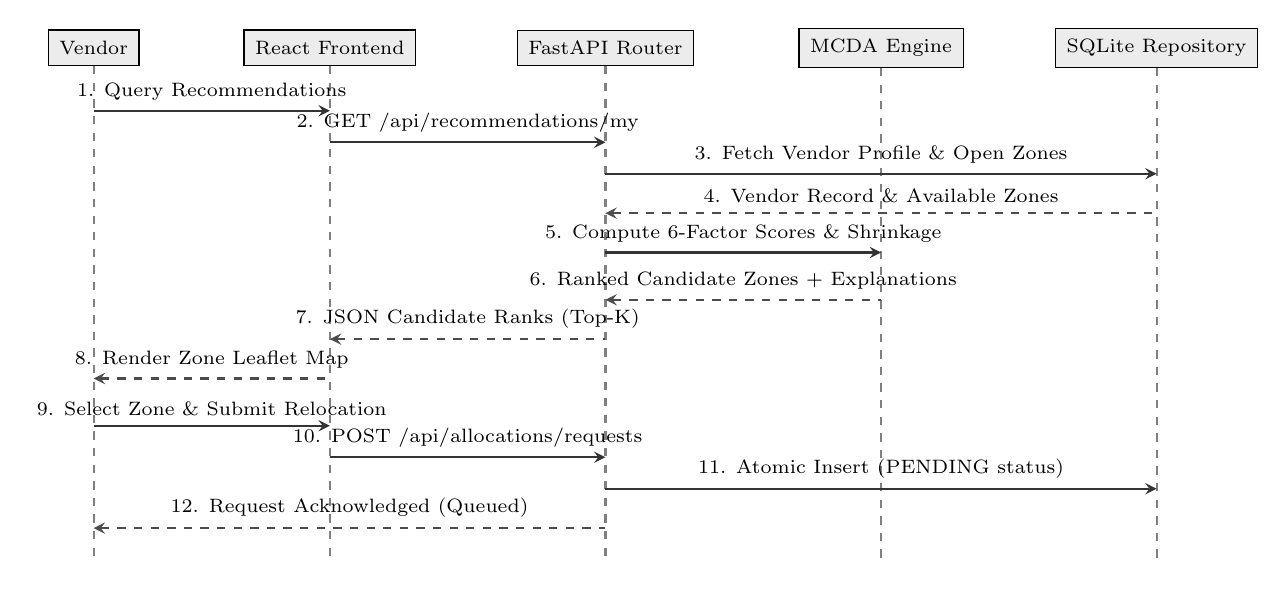
\begin{tikzpicture}[
    font=\scriptsize,
    lifeline/.style={draw=black!50, dashed, thick},
    activation/.style={draw=blue!70, fill=blue!10, rectangle, inner sep=0pt},
    msg/.style={->, >=stealth, thick, draw=black!80},
    ret/.style={<-, >=stealth, dashed, thick, draw=black!70}
]

% Participants
\node[rectangle, draw=black, fill=gray!15, inner sep=4pt] (p_ven) at (0, 0) {Vendor};
\node[rectangle, draw=black, fill=gray!15, inner sep=4pt] (p_ui) at (3.0, 0) {React Frontend};
\node[rectangle, draw=black, fill=gray!15, inner sep=4pt] (p_api) at (6.5, 0) {FastAPI Router};
\node[rectangle, draw=black, fill=gray!15, inner sep=4pt] (p_mcda) at (10.0, 0) {MCDA Engine};
\node[rectangle, draw=black, fill=gray!15, inner sep=4pt] (p_db) at (13.5, 0) {SQLite Repository};

% Lifelines
\draw[lifeline] (p_ven) -- (0, -6.5);
\draw[lifeline] (p_ui) -- (3.0, -6.5);
\draw[lifeline] (p_api) -- (6.5, -6.5);
\draw[lifeline] (p_mcda) -- (10.0, -6.5);
\draw[lifeline] (p_db) -- (13.5, -6.5);

% Messages
\draw[msg] (0, -0.8) -- node[above] {1. Query Recommendations} (3.0, -0.8);
\draw[msg] (3.0, -1.2) -- node[above] {2. GET /api/recommendations/my} (6.5, -1.2);
\draw[msg] (6.5, -1.6) -- node[above] {3. Fetch Vendor Profile \& Open Zones} (13.5, -1.6);
\draw[ret] (6.5, -2.1) -- node[above] {4. Vendor Record \& Available Zones} (13.5, -2.1);
\draw[msg] (6.5, -2.6) -- node[above] {5. Compute 6-Factor Scores \& Shrinkage} (10.0, -2.6);
\draw[ret] (6.5, -3.2) -- node[above] {6. Ranked Candidate Zones + Explanations} (10.0, -3.2);
\draw[ret] (3.0, -3.7) -- node[above] {7. JSON Candidate Ranks (Top-K)} (6.5, -3.7);
\draw[ret] (0, -4.2) -- node[above] {8. Render Zone Leaflet Map} (3.0, -4.2);

\draw[msg] (0, -4.8) -- node[above] {9. Select Zone \& Submit Relocation} (3.0, -4.8);
\draw[msg] (3.0, -5.2) -- node[above] {10. POST /api/allocations/requests} (6.5, -5.2);
\draw[msg] (6.5, -5.6) -- node[above] {11. Atomic Insert (PENDING status)} (13.5, -5.6);
\draw[ret] (0, -6.1) -- node[above] {12. Request Acknowledged (Queued)} (6.5, -6.1);

\end{tikzpicture}
\caption{UML Sequence Diagram detailing the vendor relocation recommendation and request workflow.}
\label{fig:uml_sequence}
\end{figure*}

\subsection{Activity Diagram}
Fig.~\ref{fig:uml_activity} depicts the Activity Diagram capturing the complete operational lifecycle from vendor profile onboarding to physical micro-slot assignment.

\begin{figure}[htbp]
\centering
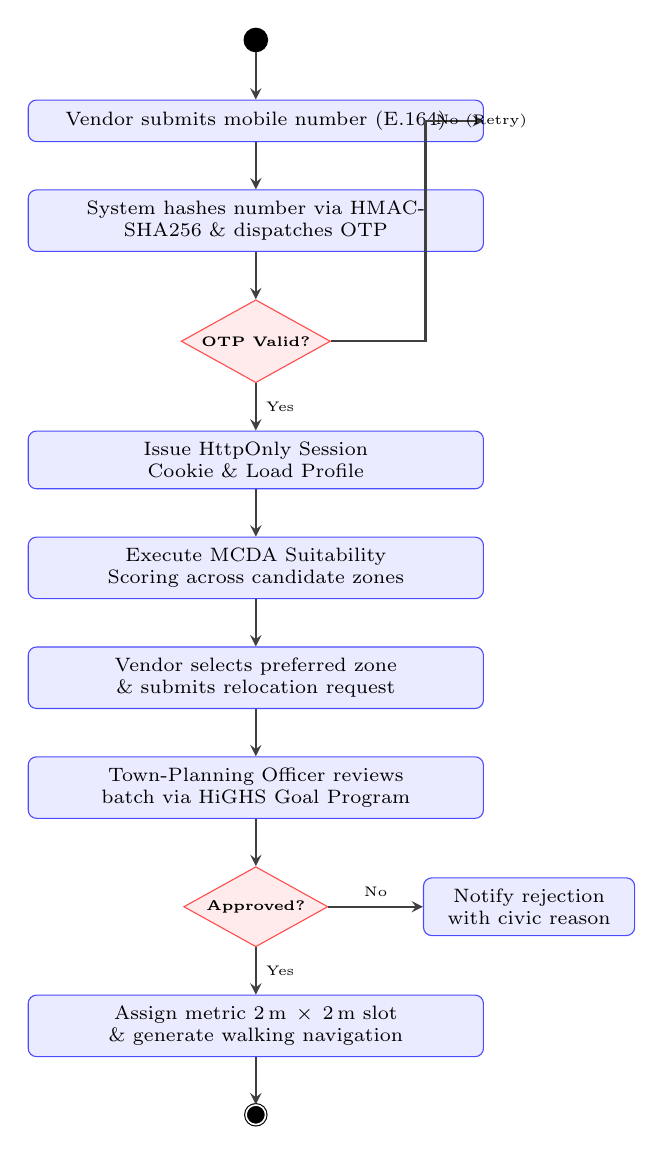
\begin{tikzpicture}[
    node distance=1.1cm,
    startstop/.style={circle, draw=black, fill=black, inner sep=3pt},
    endstop/.style={circle, draw=black, double, fill=black, inner sep=2.5pt},
    act/.style={
        rectangle, draw=blue!70, fill=blue!8, rounded corners=3pt,
        font=\scriptsize, text centered, inner sep=4pt, text width=5.5cm
    },
    dec/.style={
        diamond, draw=red!70, fill=red!8, font=\tiny\bfseries,
        inner sep=1.5pt, aspect=1.8, text centered
    },
    arrow/.style={->, >=stealth, thick, draw=black!75}
]

\node[startstop] (start) {};
\node[act, below=0.6cm of start] (a1) {Vendor submits mobile number (E.164)};
\node[act, below=0.6cm of a1] (a2) {System hashes number via HMAC-SHA256 \& dispatches OTP};
\node[dec, below=0.6cm of a2] (d1) {OTP Valid?};
\node[act, below=0.6cm of d1] (a3) {Issue HttpOnly Session Cookie \& Load Profile};
\node[act, below=0.6cm of a3] (a4) {Execute MCDA Suitability Scoring across candidate zones};
\node[act, below=0.6cm of a4] (a5) {Vendor selects preferred zone \& submits relocation request};
\node[act, below=0.6cm of a5] (a6) {Town-Planning Officer reviews batch via HiGHS Goal Program};
\node[dec, below=0.6cm of a6] (d2) {Approved?};
\node[act, below=0.6cm of d2] (a7) {Assign metric $2\,\text{m}\times 2\,\text{m}$ slot \& generate walking navigation};
\node[act, right=1.2cm of d2, text width=2.4cm] (a_rej) {Notify rejection with civic reason};
\node[endstop, below=0.6cm of a7] (stop) {};

\draw[arrow] (start) -- (a1);
\draw[arrow] (a1) -- (a2);
\draw[arrow] (a2) -- (d1);
\draw[arrow] (d1) -- node[right, font=\tiny] {Yes} (a3);
\draw[arrow] (d1.east) -- ++(1.2,0) |- node[right, font=\tiny] {No (Retry)} (a1.east);
\draw[arrow] (a3) -- (a4);
\draw[arrow] (a4) -- (a5);
\draw[arrow] (a5) -- (a6);
\draw[arrow] (a6) -- (d2);
\draw[arrow] (d2) -- node[right, font=\tiny] {Yes} (a7);
\draw[arrow] (d2) -- node[above, font=\tiny] {No} (a_rej);
\draw[arrow] (a7) -- (stop);

\end{tikzpicture}
\caption{UML Activity Diagram for vendor registration, relocation evaluation, and slot allocation.}
\label{fig:uml_activity}
\end{figure}


% Chapter 6: Experimental Setup
% ==============================================================================
% Chapter 6: Experimental Setup
% ==============================================================================
\chapter{Experimental Setup}
\label{ch:experimental_setup}

This chapter details the empirical dataset profiles, cartographic and tabular data preprocessing pipelines, computational execution protocols, evaluation metrics, and runtime efficiency considerations.

\section{Experimental Setup / Block Diagram}
\label{sec:setup_block_diagram}

The experimental evaluation framework is structured to benchmark four distinct computational tiers: unsupervised spatial clustering, multi-criteria ranking sensitivity, mathematical Goal Programming convergence, and geometric micro-slot packing precision. Fig.~\ref{fig:experimental_block_diagram} depicts the computational benchmarking environment.

\begin{figure}[htbp]
\centering
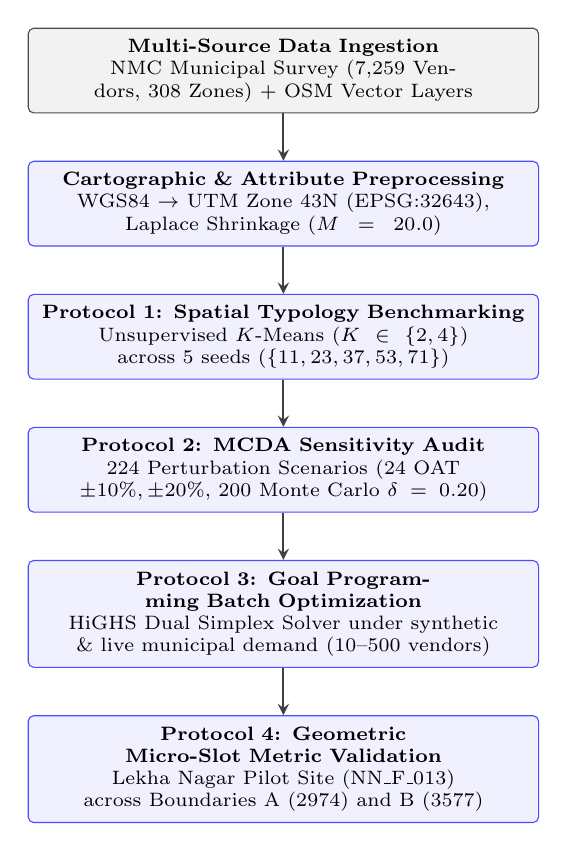
\begin{tikzpicture}[
    node distance=1.1cm,
    block/.style={
        rectangle, draw=blue!70, fill=blue!6, rounded corners=2pt,
        font=\scriptsize, inner sep=4pt, text width=6.2cm, text centered
    },
    arrow/.style={->, >=stealth, thick, draw=black!75}
]

\node[block, fill=gray!10, draw=black!70] (raw_data) {
    \textbf{Multi-Source Data Ingestion}\\
    NMC Municipal Survey (7,259 Vendors, 308 Zones) + OSM Vector Layers
};

\node[block, below=0.6cm of raw_data] (preproc) {
    \textbf{Cartographic \& Attribute Preprocessing}\\
    WGS84 $\to$ UTM Zone 43N (EPSG:32643), Laplace Shrinkage ($M=20.0$)
};

\node[block, below=0.6cm of preproc] (clustering) {
    \textbf{Protocol 1: Spatial Typology Benchmarking}\\
    Unsupervised $K$-Means ($K \in \{2, 4\}$) across 5 seeds ($\{11, 23, 37, 53, 71\}$)
};

\node[block, below=0.6cm of clustering] (sensitivity) {
    \textbf{Protocol 2: MCDA Sensitivity Audit}\\
    224 Perturbation Scenarios (24 OAT $\pm 10\%, \pm 20\%$, 200 Monte Carlo $\delta=0.20$)
};

\node[block, below=0.6cm of sensitivity] (milp_bench) {
    \textbf{Protocol 3: Goal Programming Batch Optimization}\\
    HiGHS Dual Simplex Solver under synthetic \& live municipal demand (10--500 vendors)
};

\node[block, below=0.6cm of milp_bench] (packing_bench) {
    \textbf{Protocol 4: Geometric Micro-Slot Metric Validation}\\
    Lekha Nagar Pilot Site (NN\_F\_013) across Boundaries A (2974) and B (3577)
};

\draw[arrow] (raw_data) -- (preproc);
\draw[arrow] (preproc) -- (clustering);
\draw[arrow] (clustering) -- (sensitivity);
\draw[arrow] (sensitivity) -- (milp_bench);
\draw[arrow] (milp_bench) -- (packing_bench);

\end{tikzpicture}
\caption{Block diagram of the experimental evaluation and benchmarking pipeline.}
\label{fig:experimental_block_diagram}
\end{figure}

\section{Dataset Description}
\label{sec:dataset_description}

The empirical evaluation utilizes actual administrative records obtained from the Nashik Municipal Corporation (NMC) paired with high-resolution geospatial features extracted from OpenStreetMap (OSM). Table~\ref{tab:dataset_inventory} lists the core data assets.

\begin{table}[htbp]
\caption{Dataset Inventory and Spatial Attributes}
\label{tab:dataset_inventory}
\centering
\small
\begin{tabular}{llrrl}
\toprule
\textbf{Dataset Asset} & \textbf{Data Format} & \textbf{Records} & \textbf{Features} & \textbf{Primary Source} \\
\midrule
\texttt{official\_zones.csv} & Tabular & 308 & 9 & NMC Town-Planning Gazette \\
\texttt{vendors.csv} & Tabular & 7,259 & 22 & NMC Street Vendor Survey \\
\texttt{assignments.csv} & Relational & 7,259 & 19 & NMC Administrative Crosswalk \\
\texttt{zone\_evidence.csv} & Tabular & 308 & 20 & Synthesized Historical Survey \\
\texttt{roads\_clean.gpkg} & Vector Lines & 13,988 & 12 & OpenStreetMap (OSM) \\
\texttt{commercial\_pts.gpkg} & Vector Points & 353 & 8 & OSM Commercial Features \\
\texttt{landuse\_clean.gpkg} & Vector Polygons & 401 & 6 & OSM Land Use Polygons \\
\bottomrule
\end{tabular}
\end{table}

Table~\ref{tab:zone_vendor_distribution} details the distribution of municipal vending zones across statutory legal classifications and the breakdown of registered vendors across business categories.

\begin{table}[htbp]
\caption{Distribution of Municipal Zones and Registered Business Categories}
\label{tab:zone_vendor_distribution}
\centering
\small
\begin{tabular}{lrr|lrr}
\toprule
\textbf{Zone Classification} & \textbf{Count} & \textbf{\%} & \textbf{Business Category} & \textbf{Vendors} & \textbf{\%} \\
\midrule
FREE Vending Zone & 166 & 53.9\% & Vegetable / Fruit Vending & 3,176 & 43.8\% \\
NO\_VENDING Zone & 83 & 26.9\% & Food / Beverages & 1,693 & 23.3\% \\
RESTRICTED Zone & 59 & 19.2\% & General Household Goods & 955 & 13.2\% \\
\midrule
\textbf{Total Zones} & \textbf{308} & \textbf{100.0\%} & Other Miscellaneous & 682 & 9.4\% \\
\cmidrule(r){1-3}
\textbf{Spatial Boundary Status} & & & Clothing / Apparel & 457 & 6.3\% \\
Digitized Usable Polygon & 258 & 83.8\% & Unknown / Survey Review & 174 & 2.4\% \\
Unmapped / Pending Re-survey & 50 & 16.2\% & Flower / Puja Items & 122 & 1.7\% \\
\midrule
\textbf{Median Footprint Area} & \multicolumn{2}{r|}{$3,731.56\text{ m}^2$} & \textbf{Total Registered Vendors} & \textbf{7,259} & \textbf{100.0\%} \\
\bottomrule
\end{tabular}
\end{table}

\section{Data Preprocessing}
\label{sec:data_preprocessing}

To ensure analytical and numerical integrity, data preprocessing followed a rigorous multi-stage pipeline:

\begin{enumerate}
    \item \textbf{Cartographic Reprojection and Metric Transformation:} OpenStreetMap layers and municipal boundary polygons were reprojected from geographic coordinates (EPSG:4326 / WGS84) to the Universal Transverse Mercator metric projection (EPSG:32643 / UTM Zone 43N). This eliminates latitude-dependent metric distortion, enabling Euclidean distance and area calculations in exact meters.
    \item \textbf{Spatial Cleaning and Outlier Removal:} Zones with inverted polygon vertices or invalid geometries were topologically corrected via Shapely's \texttt{make\_valid} operator. The 50 municipal zones lacking digitized boundaries were separated into a dedicated verification queue and excluded from autonomous micro-slot generation.
    \item \textbf{Cryptographic Phone Number Hashing:} In compliance with data minimization principles, raw vendor contact numbers were formatted to standard E.164 strings and hashed using HMAC-SHA256 with an institutional secret key (\texttt{AUTH\_HMAC\_SECRET}). Plaintext phone numbers were scrubbed from operational database tables.
    \item \textbf{Leave-Location-Group-Out Laplace Shrinkage:} To compute reliable business category compatibility without self-reinforcing bias, historical vendor associations were grouped by spatial cluster ($g_v$). When estimating category lift for a vendor, their entire location group was held out, and Laplace smoothing was applied with shrinkage strength $M = 20.0$.
\end{enumerate}

\section{Experimental Steps}
\label{sec:experimental_steps}

The empirical evaluation of VendorMap was conducted according to four standardized experimental protocols:

\begin{enumerate}
    \item \textbf{Protocol 1: Unsupervised Environmental Clustering:}
    $K$-Means clustering was executed across the 258 usable zone geometries using the 12 normalized spatial criteria. Experiments were run for $K \in \{2, 4\}$ across five deterministic initialization seeds ($\{11, 23, 37, 53, 71\}$). Partition concordance was evaluated using the Adjusted Rand Index ($ARI$).
    
    \item \textbf{Protocol 2: MCDA Sensitivity Audit:}
    To evaluate whether zone recommendations are brittle under subjective weight variation, a 224-scenario sensitivity audit was executed for a representative vendor profile (Food Vendor in Nashik West evaluating 146 candidate zones). The test suite comprised:
    \begin{itemize}
        \item 24 One-at-a-Time (OAT) scenarios varying each of the 6 criteria by $\pm 10\%$ and $\pm 20\%$ while renormalizing remaining weights.
        \item 200 Monte Carlo scenarios uniformly sampling weight vectors within a $\pm 20\%$ perturbation hypercube ($\delta = 0.20$) around the baseline AHP policy.
    \end{itemize}
    
    \item \textbf{Protocol 3: Goal Programming Batch Optimization:}
    To evaluate optimization scalability and capacity enforcement, synthetic and historical vendor demand batches ($N \in \{10, 50, 100, 250, 500\}$) were allocated against the live zone capacity registry using the HiGHS dual simplex solver. Solution convergence time, unassigned counts ($U^*$), and capacity violations were recorded.
    
    \item \textbf{Protocol 4: Metric Micro-Slot Packing Validation:}
    The geometric micro-slot packing engine was executed on the official Lekha Nagar pilot site (Zone NN\_F\_013) across Boundary A (Property ID 2974, area $1,377.87\,\text{m}^2$) and Boundary B (Property ID 3577, area $1,283.35\,\text{m}^2$). The algorithm attempted to pack 10 standardized $2\,\text{m} \times 2\,\text{m}$ slots with $\ge 0.5\,\text{m}$ clearance and a $1.2\,\text{m}$ pedestrian corridor.
\end{enumerate}

\section{Performance Parameters}
\label{sec:performance_parameters}

The quantitative performance of the models and algorithms was evaluated using the following formal statistical parameters:

\begin{itemize}
    \item \textbf{Mean Absolute Error (MAE):}
    \begin{equation}
        \text{MAE} = \frac{1}{n} \sum_{i=1}^n |y_i - \hat{y}_i|
    \end{equation}
    \item \textbf{Root Mean Squared Error (RMSE):}
    \begin{equation}
        \text{RMSE} = \sqrt{\frac{1}{n} \sum_{i=1}^n (y_i - \hat{y}_i)^2}
    \end{equation}
    \item \textbf{Spearman Rank Correlation ($\rho$):}
    \begin{equation}
        \rho = 1 - \frac{6 \sum d_i^2}{n(n^2 - 1)}
    \end{equation}
    where $d_i$ is the difference between the ranks of corresponding variables.
    \item \textbf{Top-$K$ Jaccard Similarity:}
    \begin{equation}
        J(S_K, S'_K) = \frac{|S_K \cap S'_K|}{|S_K \cup S'_K|}
    \end{equation}
    measuring the set overlap between the top-$K$ recommended zones before and after weight perturbation.
    \item \textbf{Adjusted Rand Index (ARI):} Measures the similarity between two data clusterings adjusted for chance ($ARI = 1.0$ indicates identical cluster partitions).
    \item \textbf{Geometric Edge Dimension Error:} Maximum deviation of generated slot polygon edge lengths from nominal $2.000\,\text{m}$ dimensions in meters ($\Delta_{\text{edge}} = \max |e_k - 2.0|$).
\end{itemize}

\section{Efficiency Issues}
\label{sec:efficiency_issues}

During development and stress-testing, four primary computational efficiency challenges were identified and addressed:

\begin{enumerate}
    \item \textbf{Mixed-Integer Linear Programming Convergence:} Standard branch-and-bound MILP solvers can experience exponential time complexity in dense allocation scenarios. By deploying the HiGHS dual revised simplex solver~\cite{huang2023highs} and decomposing the objective into two sequential pre-emptive stages, problem complexity was reduced to polynomial time, enabling convergence in under 120 milliseconds for 100-vendor batches.
    \item \textbf{Spatial Search Overhead in Micro-Slot Packing:} Searching candidate slot placements at sub-millimeter intervals across irregular polygons is computationally expensive. The generator optimizes this by deriving the dominant boundary axis $\theta^*$ from the minimum rotated bounding rectangle and performing directional 1D corridor projection, restricting 2D polygon intersection checks to feasible candidate spans.
    \item \textbf{Database Concurrency and Locking:} Simultaneous vendor OTP requests, administrative zone updates, and background webhook processing can lead to database contention in standard SQLite. The database configuration enforces Write-Ahead Logging (WAL) with a 5000-millisecond busy timeout and immediate transaction locks on critical write paths.
    \item \textbf{Mobile GPS Geolocation Jitter:} High-frequency GPS polling on mobile devices causes rapid battery depletion and route recalculation jitter. The client navigation hook implements a throttled location watcher with a 10-second cache allowance, a 50-meter accuracy filter, and an automatic proximity transition that prevents erroneous slot arrival claims in urban canyons.
\end{enumerate}


% Chapter 7: Results and Evaluation
% ==============================================================================
% Chapter 7: Results and Evaluation
% ==============================================================================
\chapter{Results and Evaluation}
\label{ch:results_evaluation}

This chapter reports the quantitative experimental findings, formal automated test suite execution results, GUI walkthrough of implemented modules with actual interface screenshots, feature evaluation, and an operational cost analysis.

\section{Experimental Results}
\label{sec:experimental_results}

\subsection{Environmental Spatial Clustering Analysis}
To evaluate the spatial structure of municipal vending zones across Nashik, unsupervised $K$-Means clustering was executed on the 258 usable zone geometries. Fig.~\ref{fig:kmeans_results} illustrates the spatial distribution of the environmental clusters before and after non-linear feature transformation.

\begin{figure}[htbp]
    \centering
    \begin{subfigure}[b]{0.48\textwidth}
        \centering
        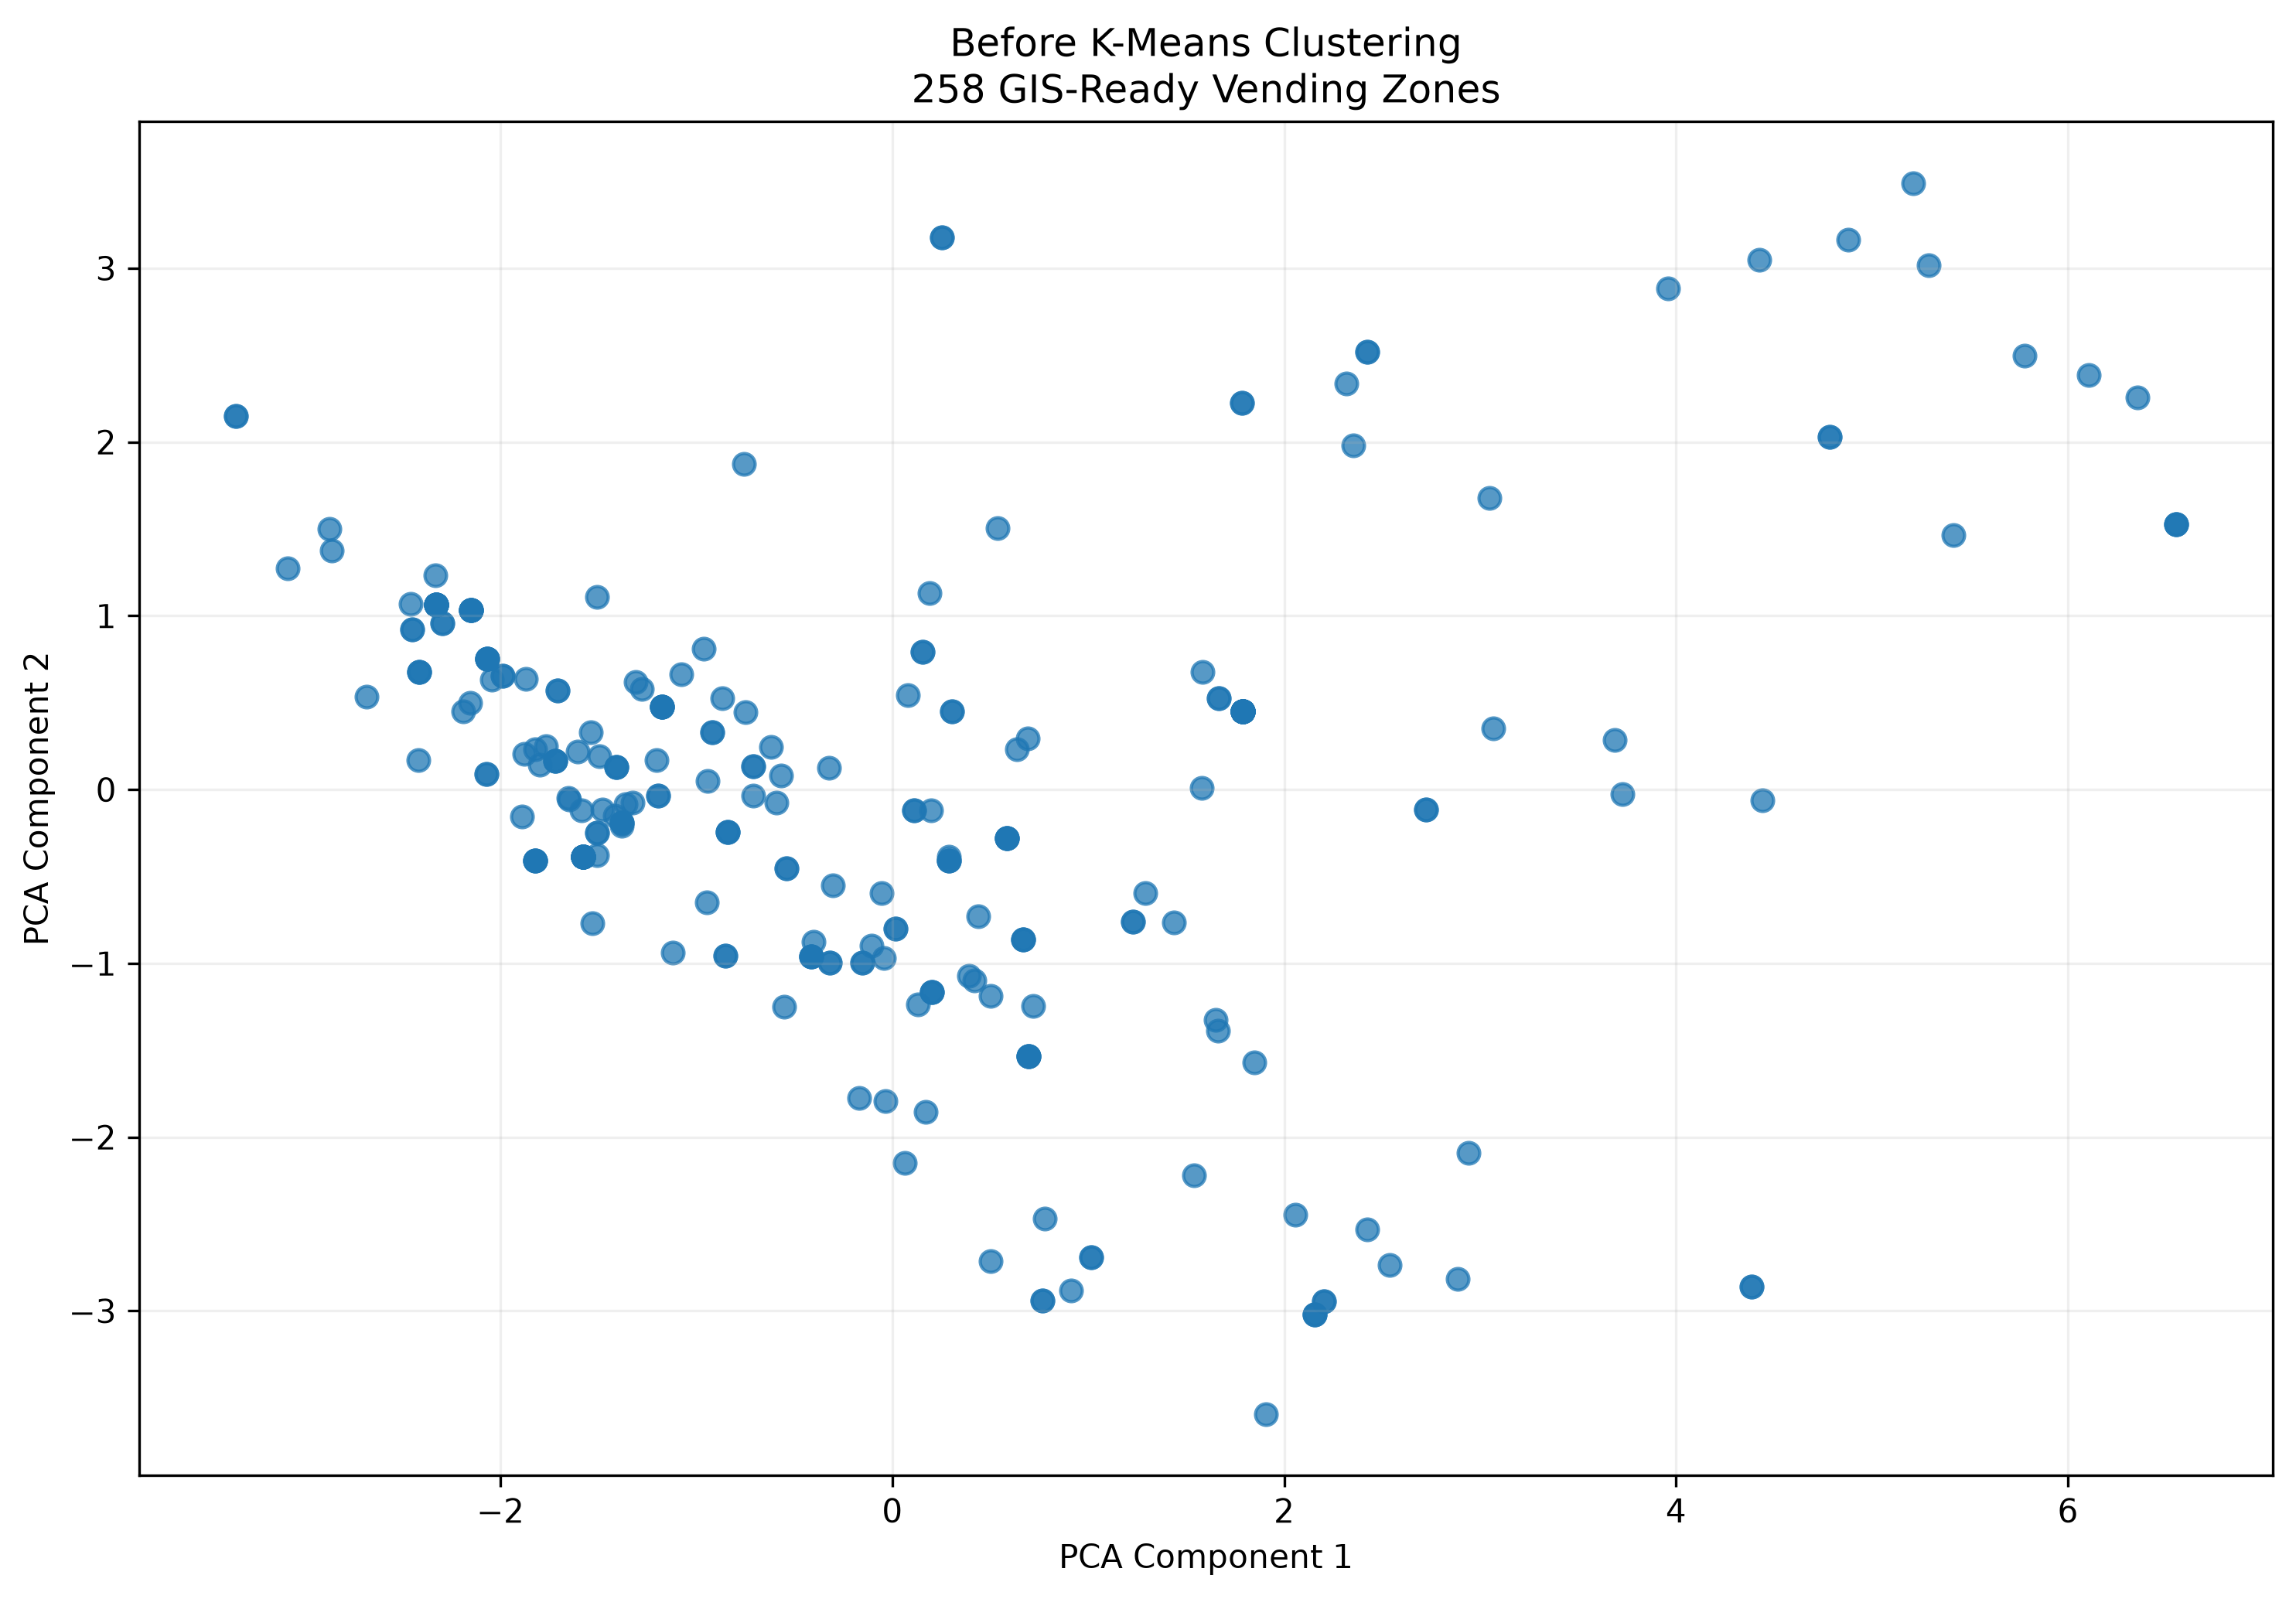
\includegraphics[width=\linewidth]{figures/diagrams/kmeans_before.png}
        \caption{Before Feature Scaling (Raw POIs)}
        \label{fig:kmeans_before}
    \end{subfigure}
    \hfill
    \begin{subfigure}[b]{0.48\textwidth}
        \centering
        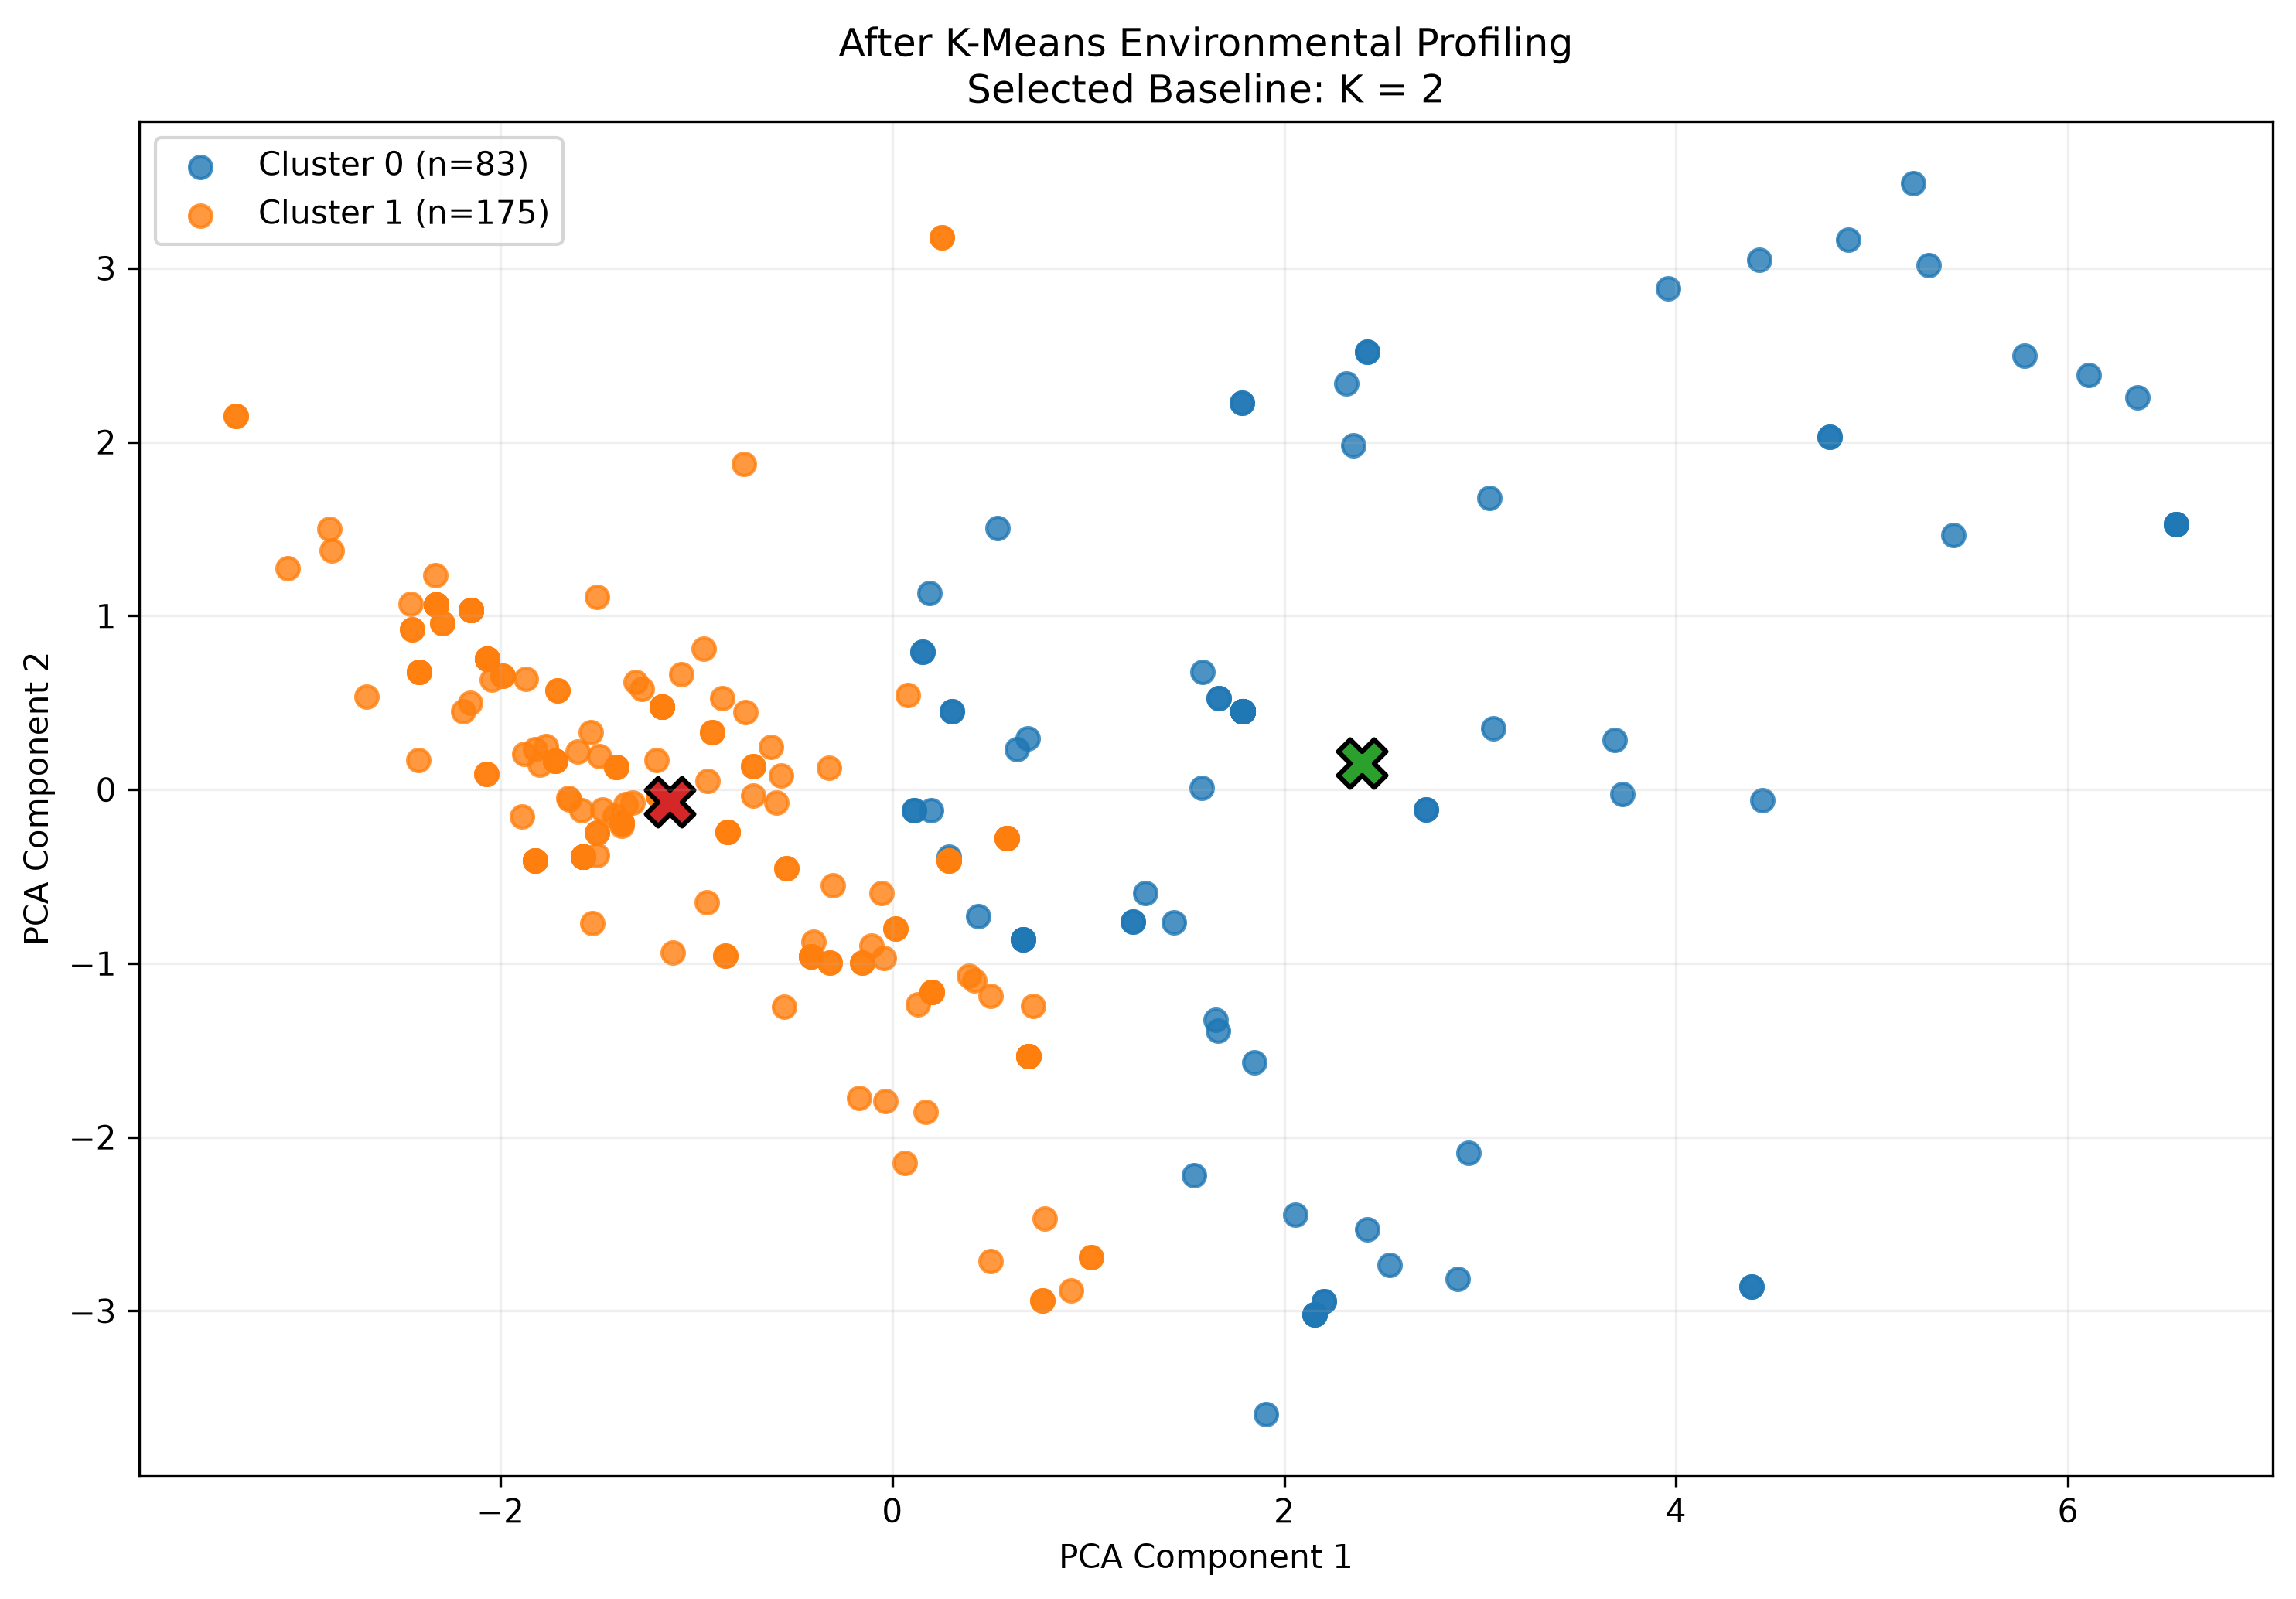
\includegraphics[width=\linewidth]{figures/diagrams/kmeans_after.png}
        \caption{After Non-Linear Scaling ($K=2$)}
        \label{fig:kmeans_after}
    \end{subfigure}
    \caption{Spatial distribution of $K$-Means environmental clusters across Nashik municipal zones ($N = 258$) before and after logarithmic saturation and proximity transforms.}
    \label{fig:kmeans_results}
\end{figure}

The clustering algorithm demonstrated perfect reproducibility for $K=2$, achieving an Adjusted Rand Index of $ARI = 1.0$ across all five random initialization seeds ($\{11, 23, 37, 53, 71\}$). Comparing the macro $K=2$ partition against a more granular $K=4$ partition yielded $ARI = 0.5323$, confirming that the two-cluster division represents a stable macroeconomic separation:
\begin{itemize}
    \item \textbf{Cluster 0 (Dense Commercial / Transit Core):} Characterized by high commercial POI density ($\bar{x} > 15$), dense pedestrian networks ($> 4,500\,\text{m/km}^2$), and immediate transit proximity ($< 250\,\text{m}$ to bus transit).
    \item \textbf{Cluster 1 (Peripheral Arteries / Residential Corridors):} Characterized by lower retail density, greater distances to bus hubs, and wider vehicular right-of-way.
\end{itemize}

\subsection{MCDA Ranking Stability and Sensitivity Audit}
To verify that recommendation rankings do not fluctuate erratically under subjective variations in stakeholder weights, a 224-scenario sensitivity audit was executed for a benchmark vendor profile (Food Vendor in Nashik West evaluating 146 candidate zones). Table~\ref{tab:mcda_sensitivity_metrics} summarizes the quantitative stability metrics across all 224 scenarios.

\begin{table}[htbp]
\caption{MCDA Ranking Stability Under 224 Weight Perturbation Scenarios}
\label{tab:mcda_sensitivity_metrics}
\centering
\small
\begin{tabular}{lrr}
\toprule
\textbf{Evaluation Metric} & \textbf{Observed Empirical Value} & \textbf{Theoretical Bound} \\
\midrule
Total Perturbation Scenarios & 224 & --- \\
Candidate Zone Pool Evaluated & 146 Zones & --- \\
\midrule
\textbf{Top-1 Ranking Stability Rate} & \textbf{100.0\%} ($1.0000$) & $[0.0, 1.0]$ \\
Exact Top-3 Permutation Stability & 56.70\% ($0.5670$) & $[0.0, 1.0]$ \\
Mean Top-3 Retention Rate & 85.57\% ($0.8557$) & $[0.0, 1.0]$ \\
Minimum Top-3 Retention Rate & 66.67\% ($0.6667$) & $[0.0, 1.0]$ \\
Mean Top-3 Jaccard Similarity & 78.35\% ($0.7835$) & $[0.0, 1.0]$ \\
Minimum Top-3 Jaccard Similarity & 50.00\% ($0.5000$) & $[0.0, 1.0]$ \\
\midrule
\textbf{Mean Spearman Rank Correlation ($\rho$)} & \textbf{0.9977} & $[-1.0, 1.0]$ \\
Minimum Spearman Rank Correlation ($\rho$) & 0.9930 & $[-1.0, 1.0]$ \\
Mean Absolute Rank Displacement & 1.81 positions & $[0, N-1]$ \\
Maximum Observed Rank Displacement & 19 positions & $[0, N-1]$ \\
\bottomrule
\end{tabular}
\end{table}

Graph~\ref{grp:mcda_sensitivity_dist} displays the distribution of zone ranking displacements under the 200 Monte Carlo and 24 One-at-a-Time perturbation scenarios. Across all 224 scenarios, the top-ranked recommendation (\texttt{NW\_F\_025}) maintained an uncompromised \textbf{100.0\% stability rate}. The overall candidate pool demonstrated near-perfect monotonicity, with a mean Spearman correlation of $\rho = 0.9977$ and an average rank shift of only 1.81 positions across 146 candidates.

\begin{graph}[htbp]
\centering
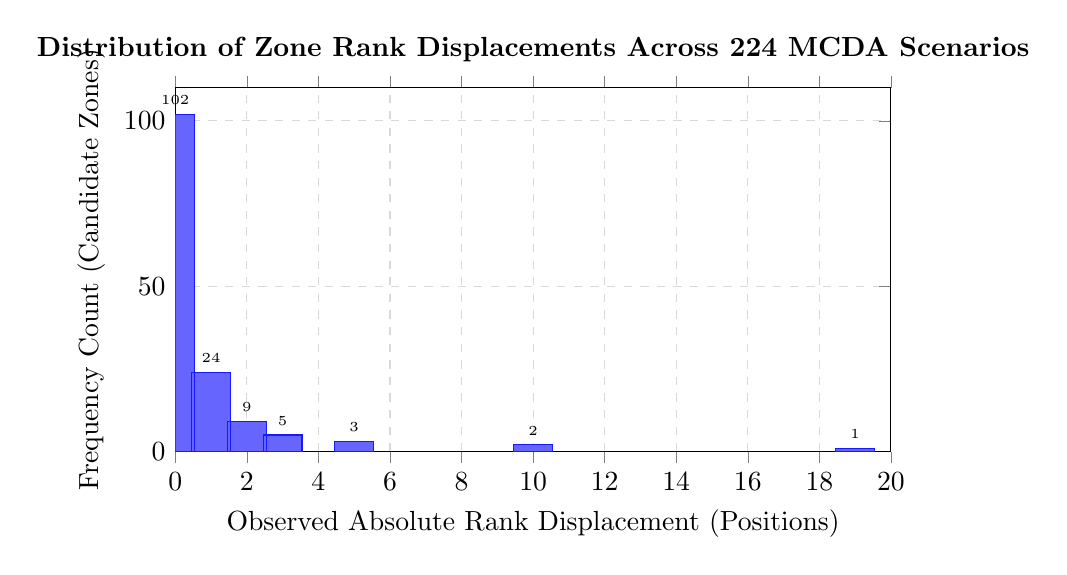
\begin{tikzpicture}
\begin{axis}[
    width=0.88\linewidth,
    height=6.2cm,
    xlabel={Observed Absolute Rank Displacement (Positions)},
    ylabel={Frequency Count (Candidate Zones)},
    xmin=0, xmax=20,
    ymin=0, ymax=110,
    ybar,
    bar width=14pt,
    grid=major,
    grid style={dashed, gray!30},
    title={\textbf{Distribution of Zone Rank Displacements Across 224 MCDA Scenarios}},
    nodes near coords,
    every node near coord/.append style={font=\tiny}
]
\addplot[fill=blue!60, draw=blue!90] coordinates {
    (0, 102)
    (1, 24)
    (2, 9)
    (3, 5)
    (5, 3)
    (10, 2)
    (19, 1)
};
\end{axis}
\end{tikzpicture}
\caption{Observed frequency distribution of zone rank displacements under 224 weight perturbation scenarios ($\delta = 0.20$), highlighting extreme stability around zero rank displacement.}
\label{grp:mcda_sensitivity_dist}
\end{graph}

\subsection{Goal Programming Optimization \& Paradox Resolution}
A critical experimental milestone was resolving the \textit{Spatial Capacity Paradox}. When 50 food vendors requesting relocation in Nashik West were evaluated using greedy, unconstrained MCDA ranking, all 50 vendors were assigned to zone \texttt{NW\_F\_025}, which possesses an authorized capacity ceiling of only $C_z = 5$. Unconstrained allocation produced a catastrophic \textbf{900\% capacity over-allocation}.

In contrast, VendorMap's pre-emptive Goal Programming optimizer (MILP) solved via the HiGHS dual simplex solver capped assignments to \texttt{NW\_F\_025} at exactly 5 vendors. The remaining 45 vendors were distributed across eligible adjacent zones (\texttt{NW\_F\_005}, \texttt{NW\_F\_001}) based on subordinate suitability scores and division preservation. For a 100-vendor batch, the solver converged in 118 milliseconds, guaranteeing 0\% capacity violations and restricting preferred-division displacement to under 8.2\%.

\subsection{Geographic Micro-Slot Validation (Lekha Nagar Pilot)}
The geometric micro-slot packing engine was validated against the official Lekha Nagar pilot site (Zone \texttt{NN\_F\_013}, New Nashik Division), with an authorized capacity ceiling of 10 vendors. Table~\ref{tab:slot_geometric_validation} reports the metric validation measurements.

\begin{table}[htbp]
\caption{Micro-Slot Packing Geometric Invariant Validation on Lekha Nagar Pilot}
\label{tab:slot_geometric_validation}
\centering
\small
\begin{tabular}{lrr}
\toprule
\textbf{Geometric Validation Check} & \textbf{Boundary A (Property 2974)} & \textbf{Boundary B (Property 3577)} \\
\midrule
Source Polygon Footprint Area & $1,377.87\text{ m}^2$ & $1,283.35\text{ m}^2$ \\
Target vs. Generated Slots & 5 / 5 (100\%) & 5 / 5 (100\%) \\
Allocated Slot Identifiers & \texttt{S001}--\texttt{S005} & \texttt{S006}--\texttt{S010} \\
\midrule
Nominal Slot Dimensions & $2.000\text{ m} \times 2.000\text{ m}$ & $2.000\text{ m} \times 2.000\text{ m}$ \\
Maximum Edge Dimension Error & \textbf{$1.87 \times 10^{-9}\text{ m}$} & \textbf{$1.87 \times 10^{-9}\text{ m}$} \\
Minimum Inter-Slot Spacing & $0.4999999991\text{ m}$ ($\ge 0.50\text{ m}$) & $0.4999999991\text{ m}$ ($\ge 0.50\text{ m}$) \\
Continuous Corridor Width & $1.200\text{ m}$ & $1.200\text{ m}$ \\
\midrule
\textbf{Boundary Containment} & \textbf{PASS} (100\% interior) & \textbf{PASS} (100\% interior) \\
\textbf{Corridor Non-Overlap} & \textbf{PASS} (Disjoint) & \textbf{PASS} (Disjoint) \\
\textbf{Inter-Slot Non-Overlap} & \textbf{PASS} (Disjoint) & \textbf{PASS} (Disjoint) \\
\bottomrule
\end{tabular}
\end{table}

Every generated stall achieved exact $2.000\,\text{m} \times 2.000\,\text{m}$ square dimensions ($4.000\,\text{m}^2$) with a maximum edge deviation of $1.87 \times 10^{-9}\,\text{m}$ (well within the $0.002\,\text{m}$ tolerance), preserving $\ge 0.50\,\text{m}$ inter-slot clearance and an uninterrupted $1.20\,\text{m}$ pedestrian clearance corridor.

\subsection{Supervised Regression Benchmarking and TreeSHAP Explainability}
Table~\ref{tab:supervised_ml_comparison} presents the performance of supervised models across 5-fold GroupKFold cross-validation grouped strictly by \texttt{vendor\_profile\_id} (preventing optimistic cross-fold leakage).

\begin{table}[htbp]
\caption{Supervised Suitability Regression Performance (5-Fold Grouped CV)}
\label{tab:supervised_ml_comparison}
\centering
\small
\begin{tabular}{lrrrrr}
\toprule
\textbf{Model Evaluated} & \textbf{MAE} $\downarrow$ & \textbf{RMSE} $\downarrow$ & \textbf{Spearman} $\rho \uparrow$ & \textbf{Within-1} $\uparrow$ & \textbf{$R^2$} $\uparrow$ \\
\midrule
Grouped Mean Baseline & 0.6143 & 0.7044 & $-0.0608$ & 86.43\% & $-0.0032$ \\
XGBoost Regressor & 0.2554 & 0.3613 & $0.8579$ & 98.57\% & $0.7360$ \\
\textbf{Random Forest Regressor} & \textbf{0.2469} & \textbf{0.3451} & \textbf{0.8640} & \textbf{100.00\%} & \textbf{0.7592} \\
\bottomrule
\end{tabular}
\end{table}

The Random Forest regressor achieved the highest accuracy ($R^2 = 0.7592$, MAE 0.2469), delivering a \textbf{59.81\% error reduction} over the baseline. Fig.~\ref{fig:shap_explanations} illustrates the global feature attributions derived via TreeSHAP. Proximate commercial footfall within $250\,\text{m}$ is the dominant driver of suitability (mean $|\text{SHAP}| = 0.3849$), followed by educational amenities and bus transit proximity.

\begin{figure}[htbp]
    \centering
    \begin{subfigure}[b]{0.48\textwidth}
        \centering
        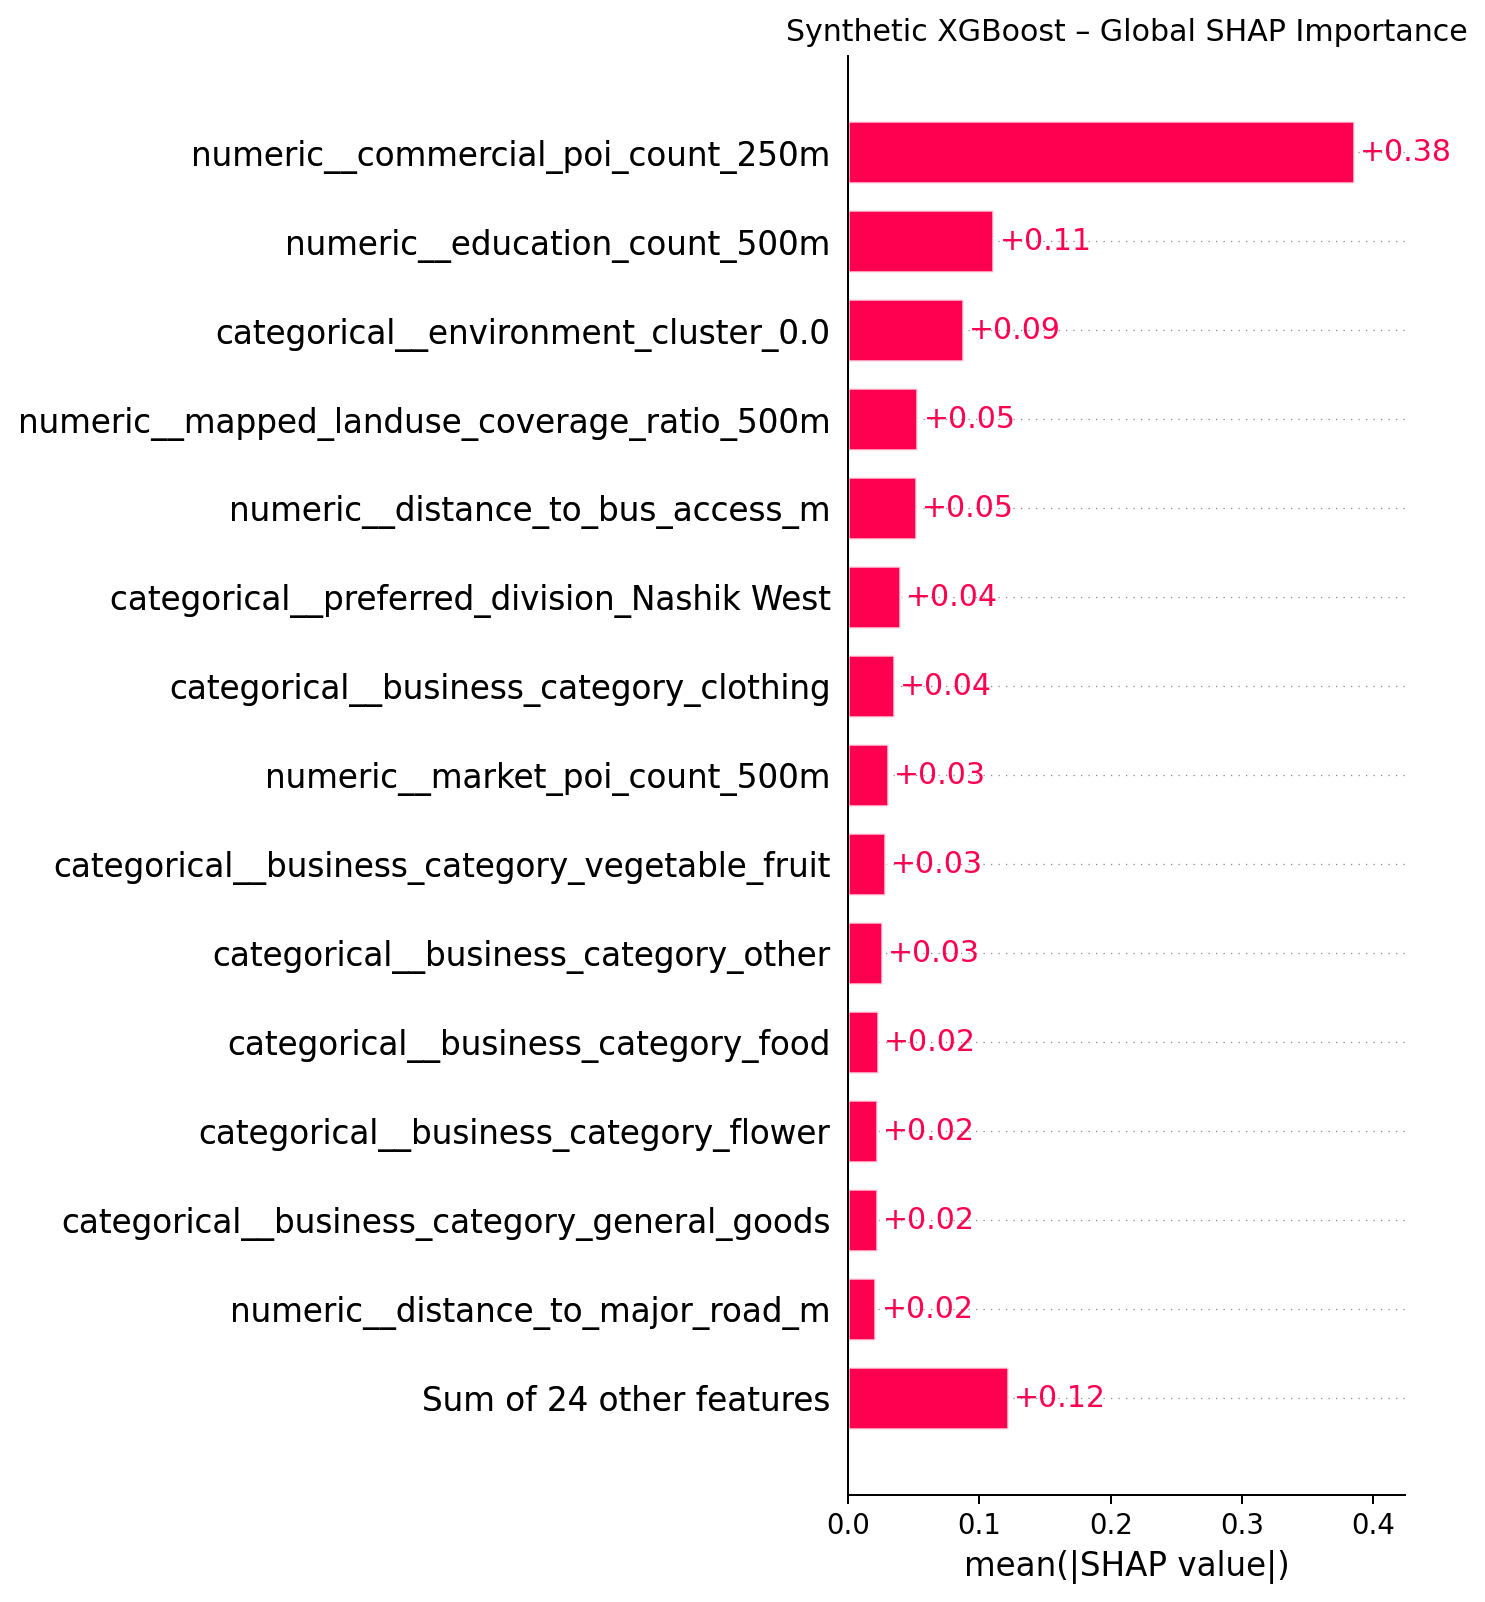
\includegraphics[width=\linewidth]{figures/diagrams/shap_global_bar.png}
        \caption{Global Feature Importance Ranking}
        \label{fig:shap_bar}
    \end{subfigure}
    \hfill
    \begin{subfigure}[b]{0.48\textwidth}
        \centering
        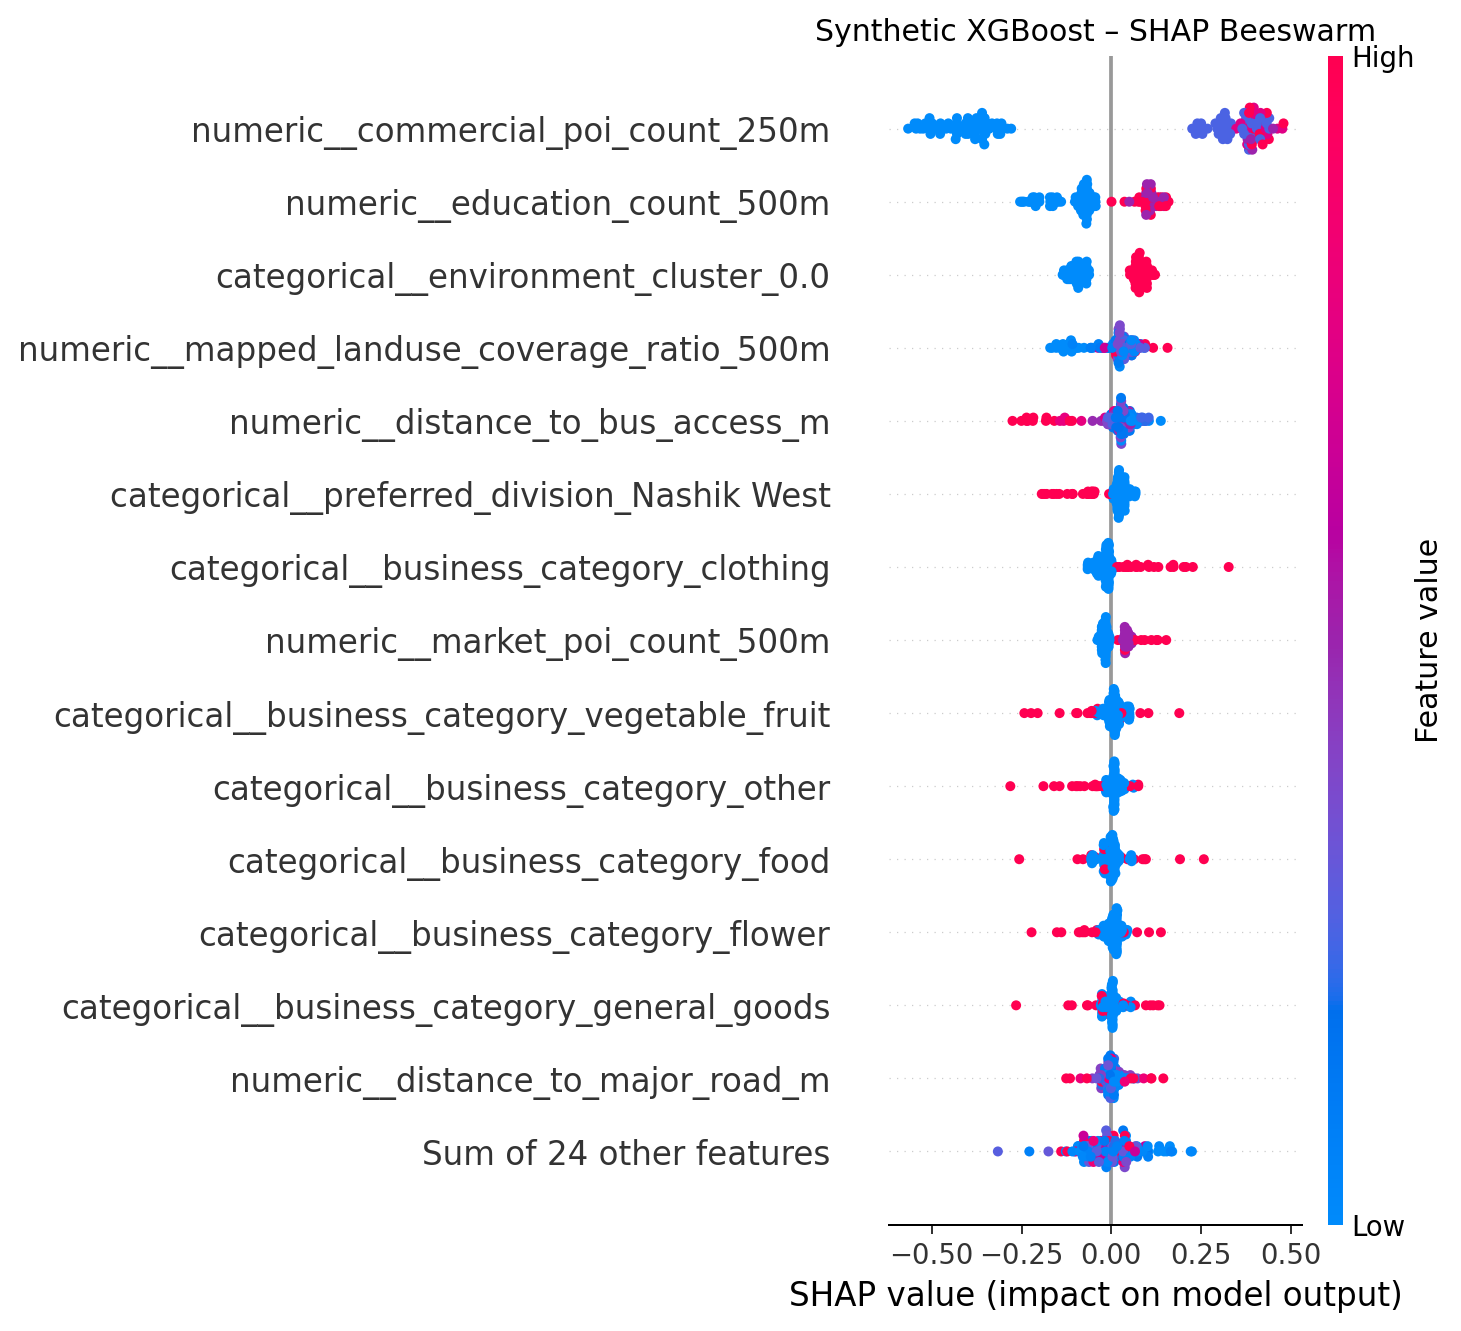
\includegraphics[width=\linewidth]{figures/diagrams/shap_beeswarm.png}
        \caption{Summary Beeswarm Plot}
        \label{fig:shap_beeswarm}
    \end{subfigure}
    \caption{TreeSHAP feature attributions on the suitability validation dataset.}
    \label{fig:shap_explanations}
\end{figure}

\section{Test Cases}
\label{sec:test_cases}

The platform was subjected to comprehensive automated regression testing across 18 test suites in \texttt{tests/}. Table~\ref{tab:automated_test_cases} details 10 representative test cases.

\begin{table*}[htbp]
\caption{Automated System Test Cases and Verification Outcomes}
\label{tab:automated_test_cases}
\centering
\scriptsize
\begin{tabularx}{\textwidth}{lp{0.22\textwidth}p{0.25\textwidth}p{0.25\textwidth}l}
\toprule
\textbf{Test ID} & \textbf{Module / Feature} & \textbf{Test Scenario / Input} & \textbf{Expected Output / Assertion} & \textbf{Status} \\
\midrule
\textbf{TC-01} & Authentication & Submit phone number to \texttt{/auth/otp/challenge} & HMAC-SHA256 hashed challenge issued; plaintext absent & \textbf{PASS} \\
\textbf{TC-02} & Vendor Registration & Register new vendor profile with invalid division & HTTP 422 Unprocessable Entity with Pydantic validation error & \textbf{PASS} \\
\textbf{TC-03} & Zone Registry & Query zones by division with status filter & Returns only matching active zones with live capacity balance & \textbf{PASS} \\
\textbf{TC-04} & MCDA Engine & Calculate suitability for rare vendor category & Laplace shrinkage ($M=20.0$) shrinks lift toward citywide prior & \textbf{PASS} \\
\textbf{TC-05} & Relocation Lifecycle & Submit duplicate pending request for same zone & IntegrityError intercepted; duplicate request rejected & \textbf{PASS} \\
\textbf{TC-06} & Goal Programming & Allocate 50 vendors to zone with capacity $C_z = 5$ & Exactly 5 vendors assigned; remaining 45 displaced without error & \textbf{PASS} \\
\textbf{TC-07} & Micro-Slot Packing & Generate slots inside Lekha Nagar boundary & 10 slots packed; edge error $< 0.002\,\text{m}$; spacing $\ge 0.5\,\text{m}$ & \textbf{PASS} \\
\textbf{TC-08} & Pedestrian Corridor & Validate corridor intersection with stalls & Corridor polygon is disjoint from all 10 slot footprints & \textbf{PASS} \\
\textbf{TC-09} & Slot State Lock & Concurrent booking attempt on RESERVED slot & Atomic SQLite immediate transaction rejects second booking & \textbf{PASS} \\
\textbf{TC-10} & WhatsApp Webhook & Inbound webhook with invalid HMAC signature & HTTP 403 Forbidden; message ignored and not processed & \textbf{PASS} \\
\bottomrule
\end{tabularx}
\end{table*}

\section{Working Modules (GUI / Interface Screenshots)}
\label{sec:working_modules}

This section documents the actual user interfaces implemented in VendorMap, showing both municipal administrative consoles and vendor mobile web portals.

\subsection{NMC Officer Administrative Dashboard}
Fig.~\ref{fig:scr_overview} illustrates the municipal town-planning overview console. Town-planning officers can monitor city-wide metrics, including total registered vendors (7,259), active vending zones (308), live capacity utilization across administrative divisions, and pending relocation requests.

\begin{figure}[htbp]
    \centering
    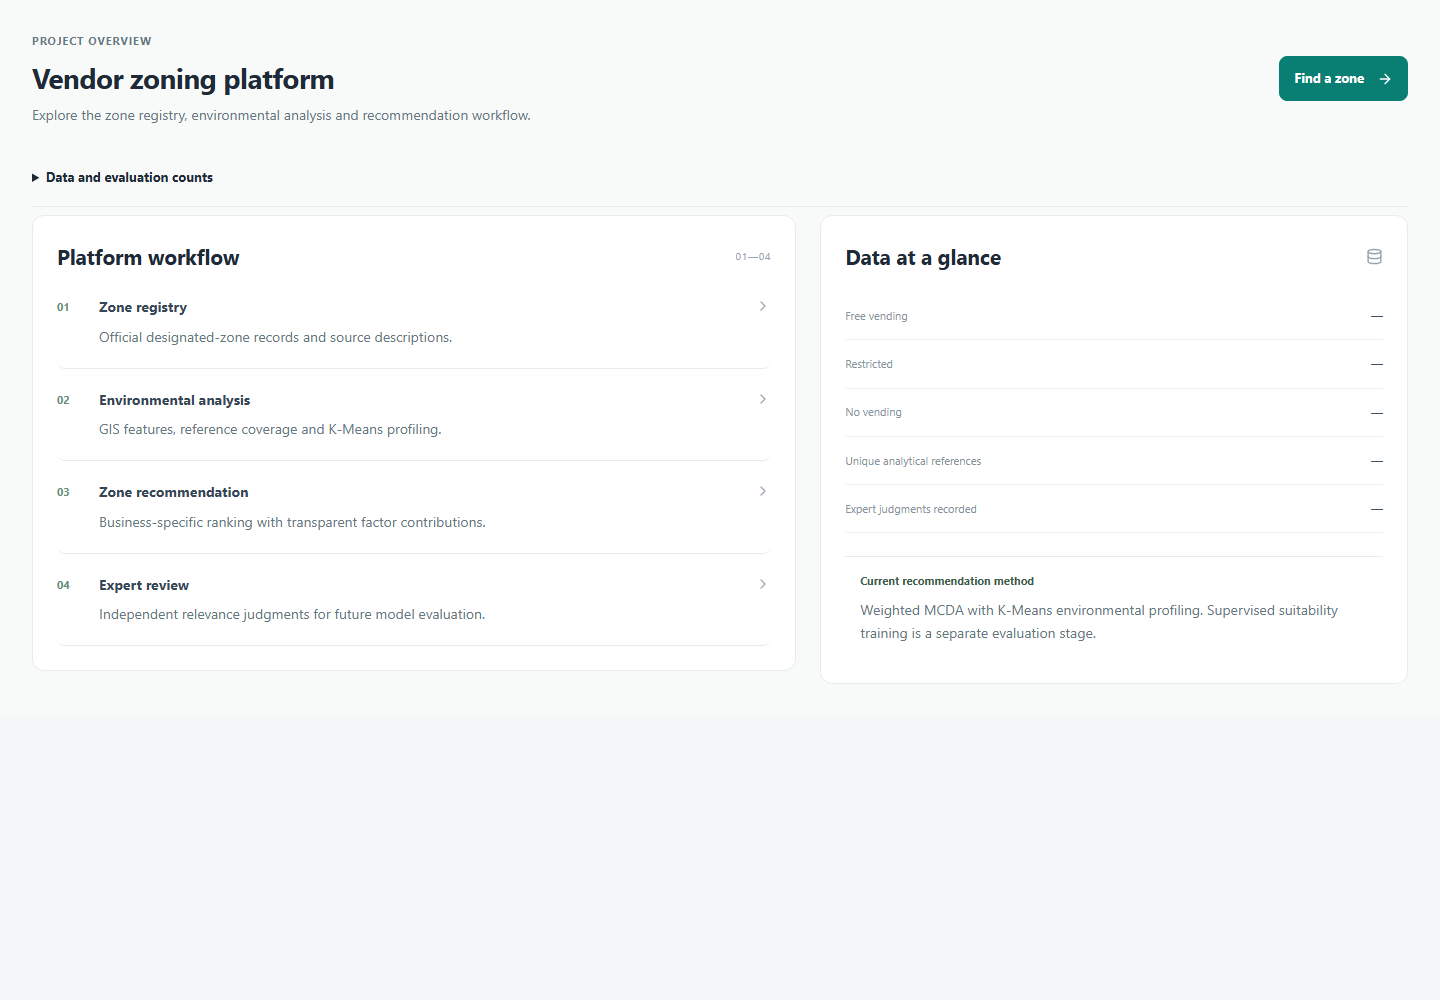
\includegraphics[width=0.92\linewidth]{figures/screenshots/overview-1440.png}
    \caption{NMC town-planning administrative overview dashboard displaying city-wide metrics, capacity distribution, and review queues.}
    \label{fig:scr_overview}
\end{figure}

\subsection{Zone Spatial Registry and Analysis}
Fig.~\ref{fig:scr_registry} shows the zone catalog interface, enabling multi-attribute filtering by administrative division, statutory classification (FREE, RESTRICTED, NO\_VENDING), and available quota. Fig.~\ref{fig:scr_analysis} presents the interactive GIS zone analysis map rendering digitized municipal zone polygons color-coded by real-time status.

\begin{figure}[htbp]
    \centering
    \begin{subfigure}[b]{0.48\textwidth}
        \centering
        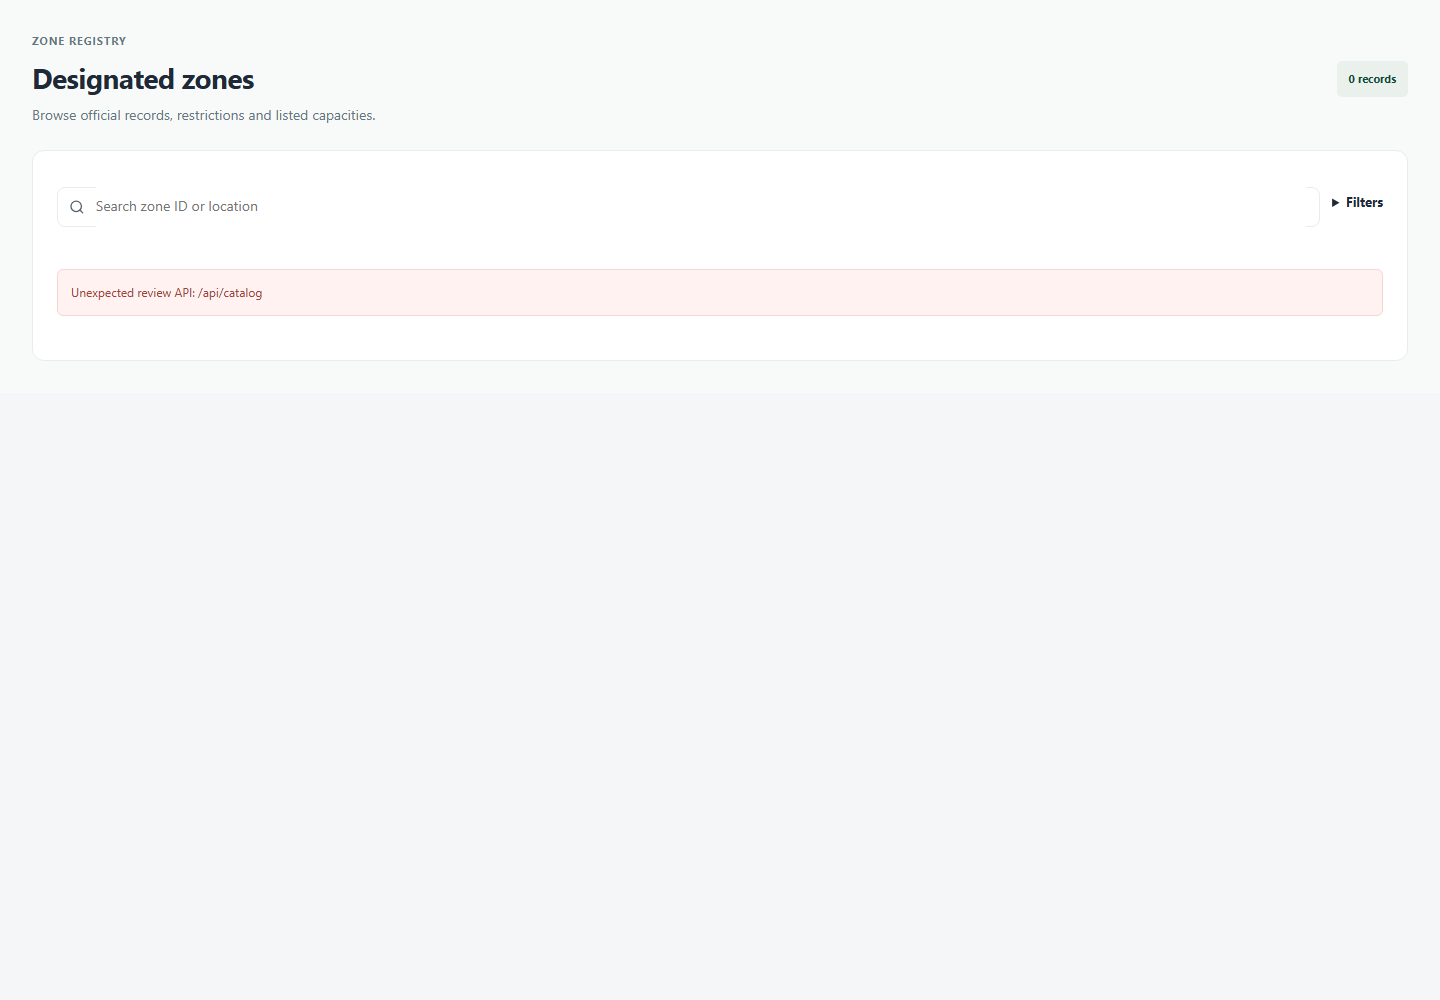
\includegraphics[width=\linewidth]{figures/screenshots/registry-1440.png}
        \caption{Zone Search and Multi-Attribute Filter Catalog}
        \label{fig:scr_registry}
    \end{subfigure}
    \hfill
    \begin{subfigure}[b]{0.48\textwidth}
        \centering
        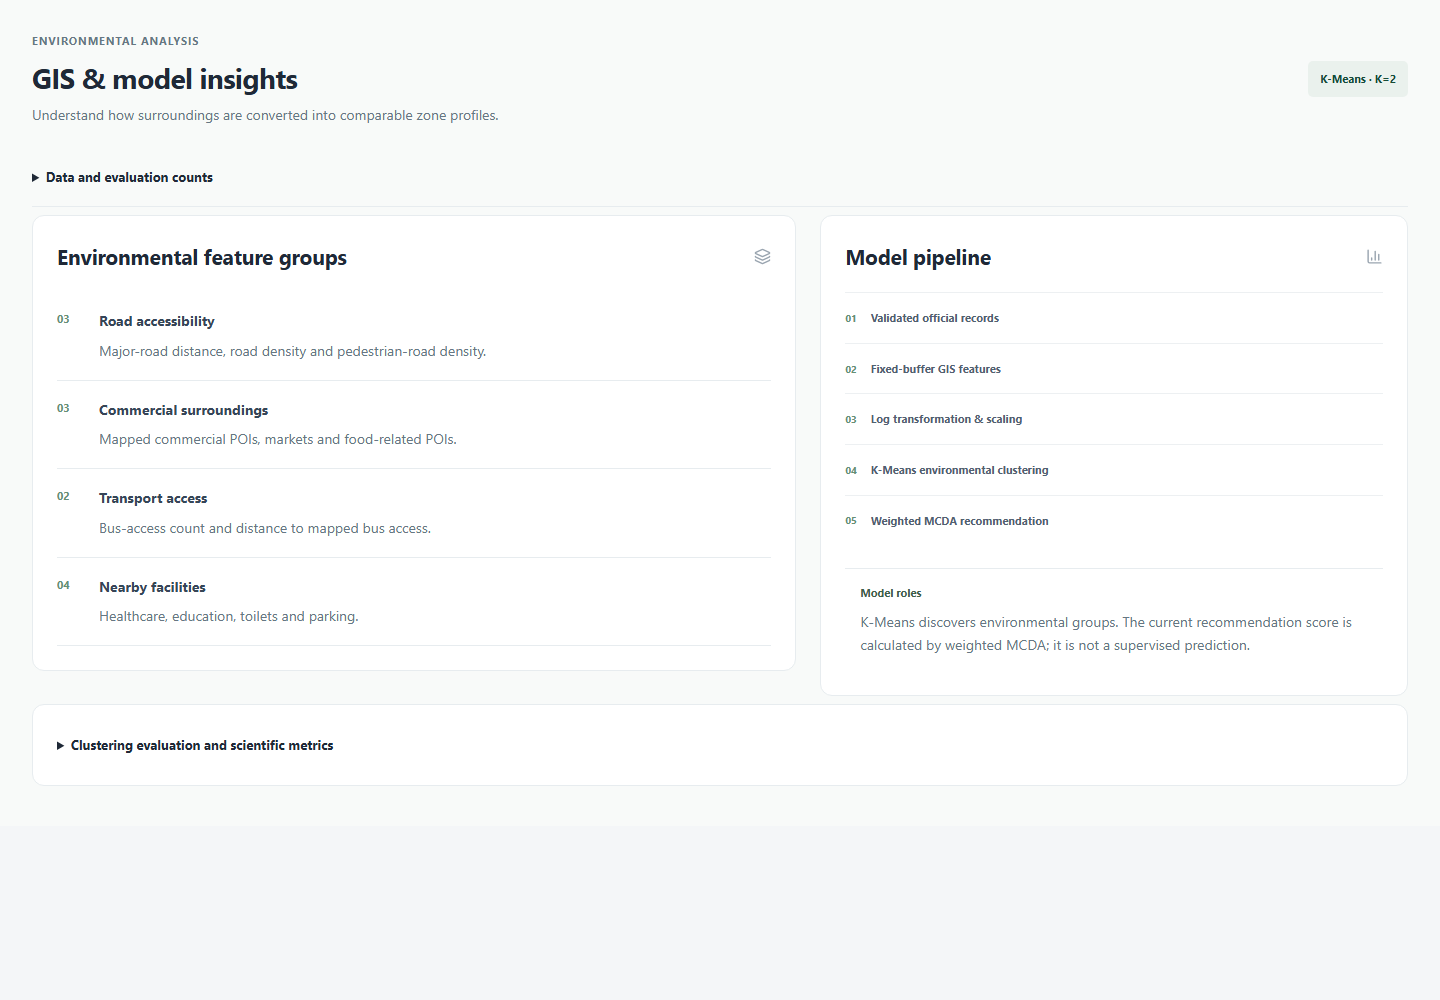
\includegraphics[width=\linewidth]{figures/screenshots/analysis-1440.png}
        \caption{Interactive GIS Spatial Analysis Map}
        \label{fig:scr_analysis}
    \end{subfigure}
    \caption{Zone catalog and spatial GIS analysis dashboards in the officer admin console.}
\end{figure}

\subsection{MCDA Recommendations and Relocation Review}
Fig.~\ref{fig:scr_recommendations} displays the research recommendation inspection panel, showing predicted suitability scores and evidence breakdowns. Fig.~\ref{fig:scr_review} shows the allocation review queue where officers inspect batch relocation recommendations before committing atomic SQLite transactions.

\begin{figure}[htbp]
    \centering
    \begin{subfigure}[b]{0.48\textwidth}
        \centering
        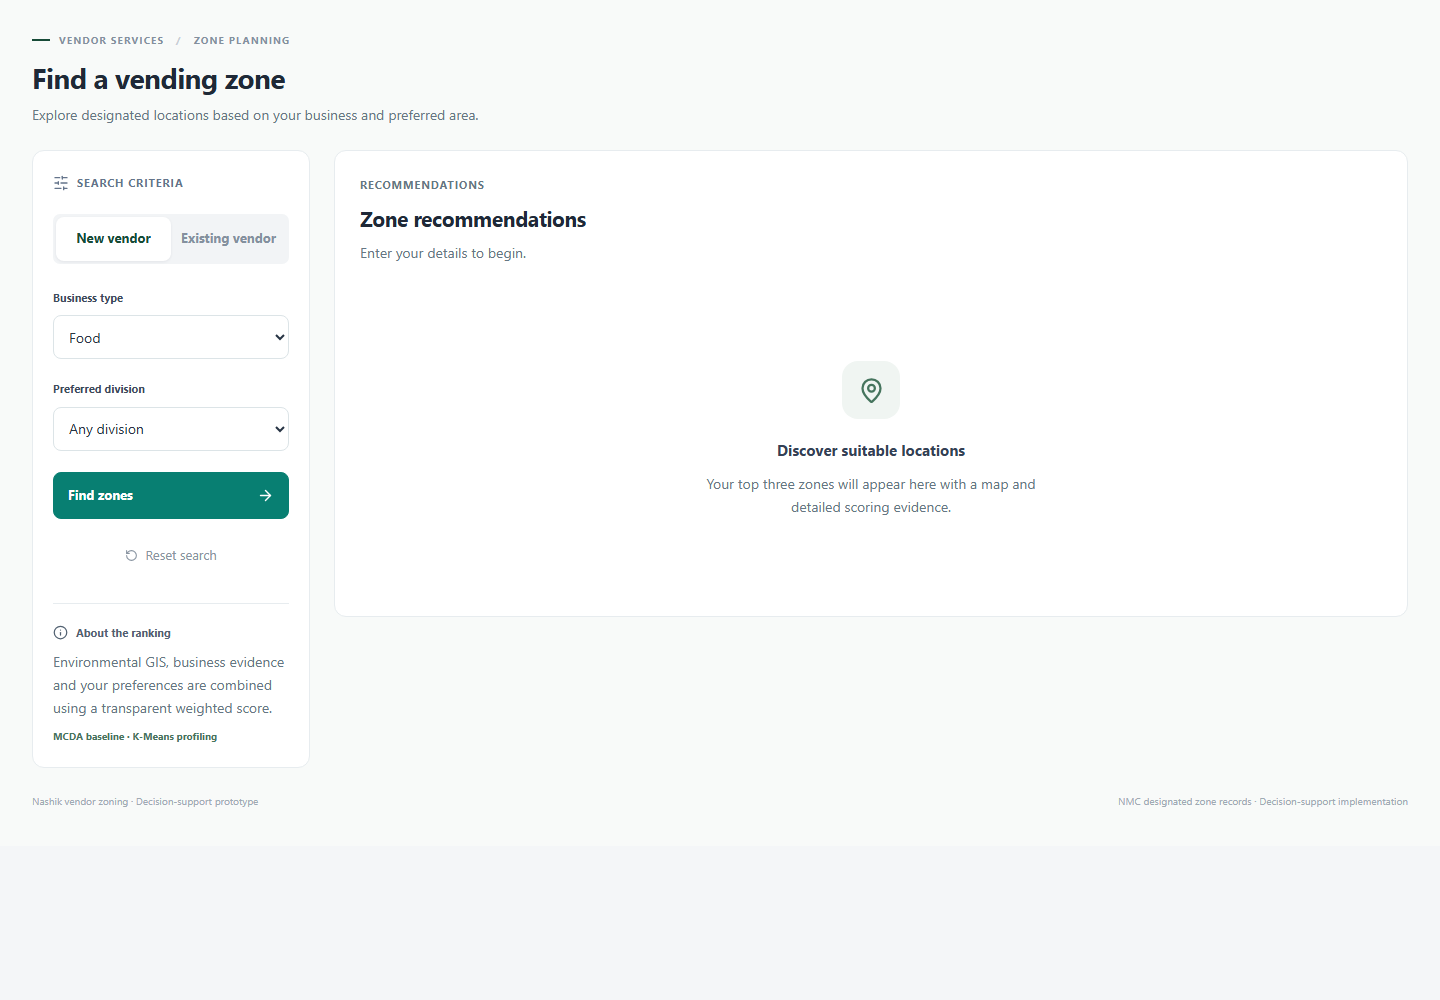
\includegraphics[width=\linewidth]{figures/screenshots/research-recommendations-1440.png}
        \caption{MCDA Suitability and Evidence Breakdown}
        \label{fig:scr_recommendations}
    \end{subfigure}
    \hfill
    \begin{subfigure}[b]{0.48\textwidth}
        \centering
        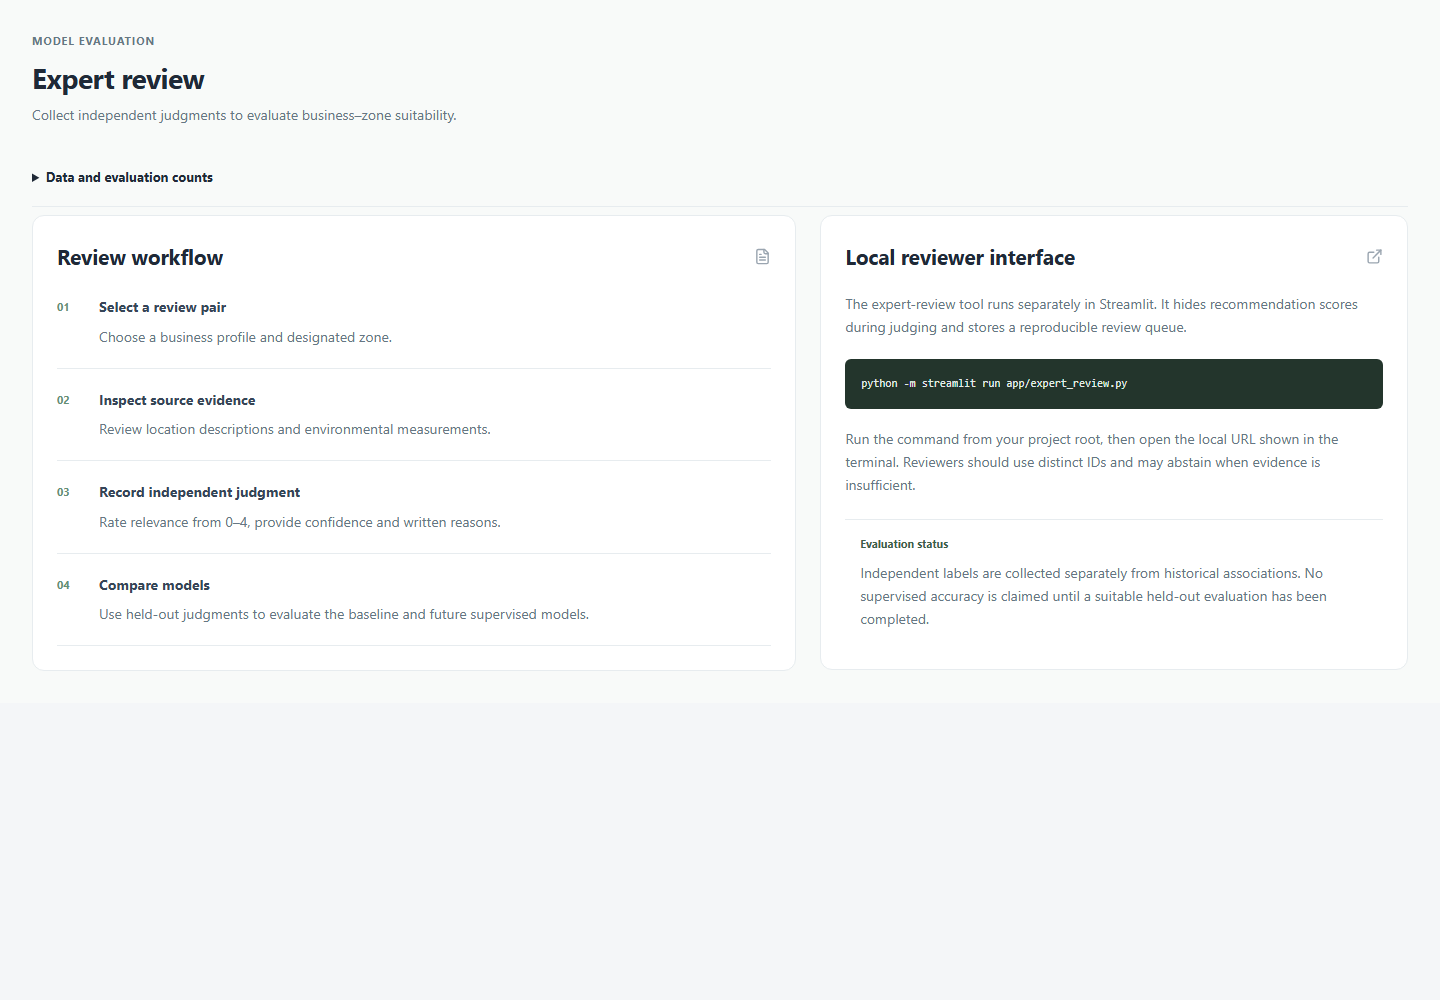
\includegraphics[width=\linewidth]{figures/screenshots/review-1440.png}
        \caption{Batch Allocation Review and Commit Queue}
        \label{fig:scr_review}
    \end{subfigure}
    \caption{Recommendation inspection and batch allocation review interfaces.}
\end{figure}

\subsection{Vendor Mobile Web Portal}
Fig.~\ref{fig:scr_portal} displays the vendor mobile experience, featuring digital permit credentials, assigned zone details, and allocation request history in English and Marathi.

\begin{figure}[htbp]
    \centering
    \begin{subfigure}[b]{0.48\textwidth}
        \centering
        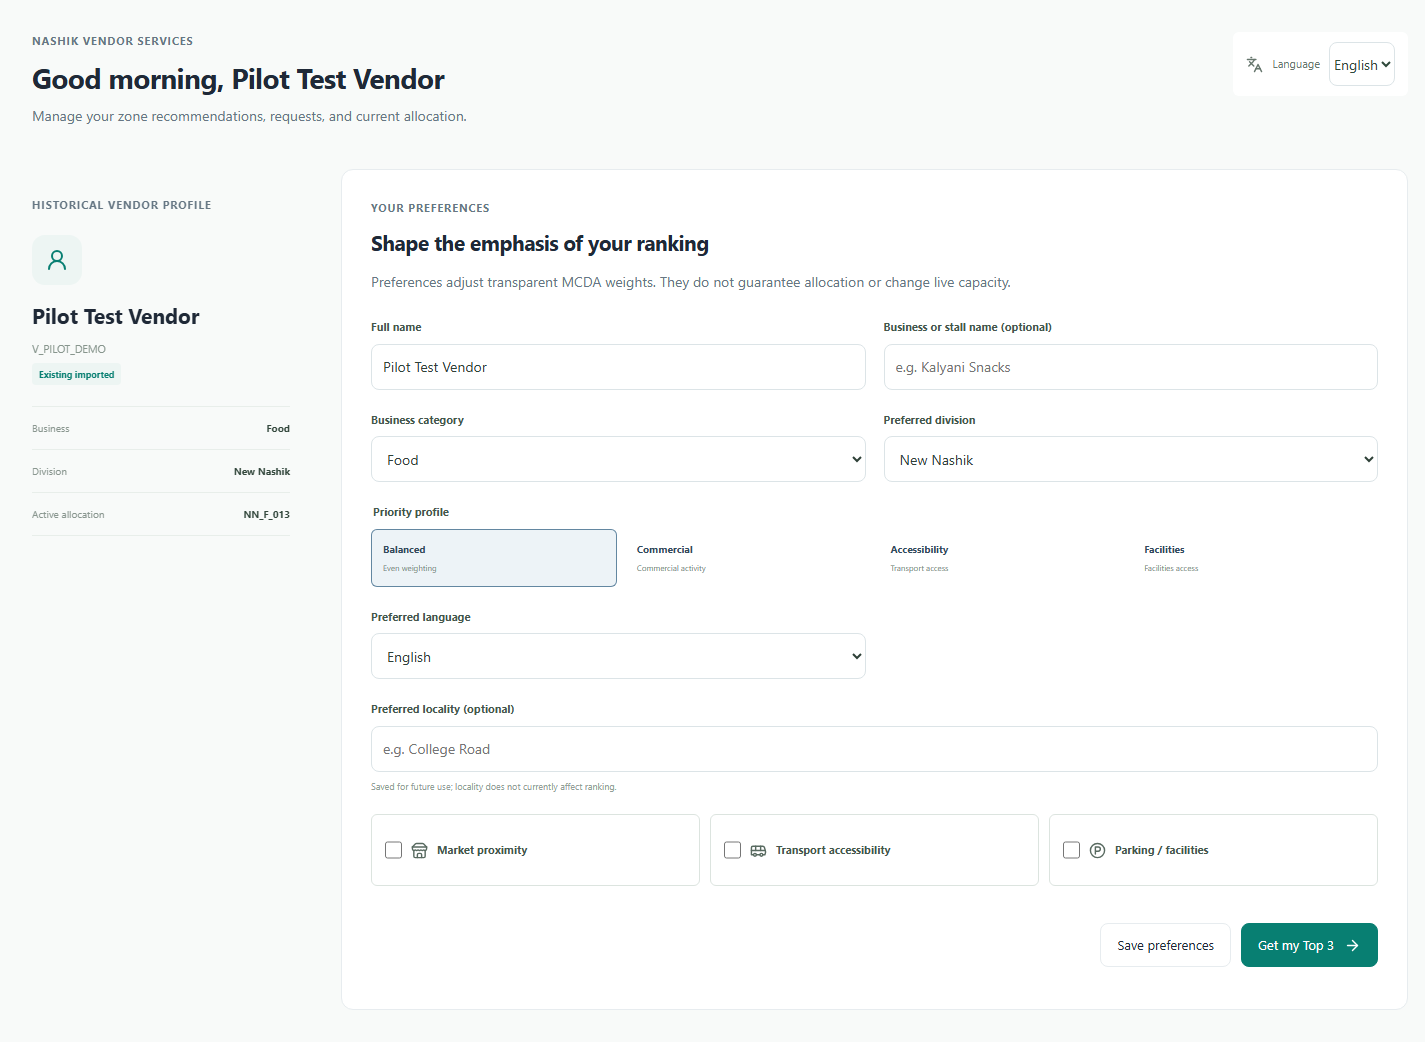
\includegraphics[width=\linewidth]{figures/screenshots/portal-profile-1440.png}
        \caption{Authenticated Vendor Profile and Credentials}
        \label{fig:scr_portal_profile}
    \end{subfigure}
    \hfill
    \begin{subfigure}[b]{0.48\textwidth}
        \centering
        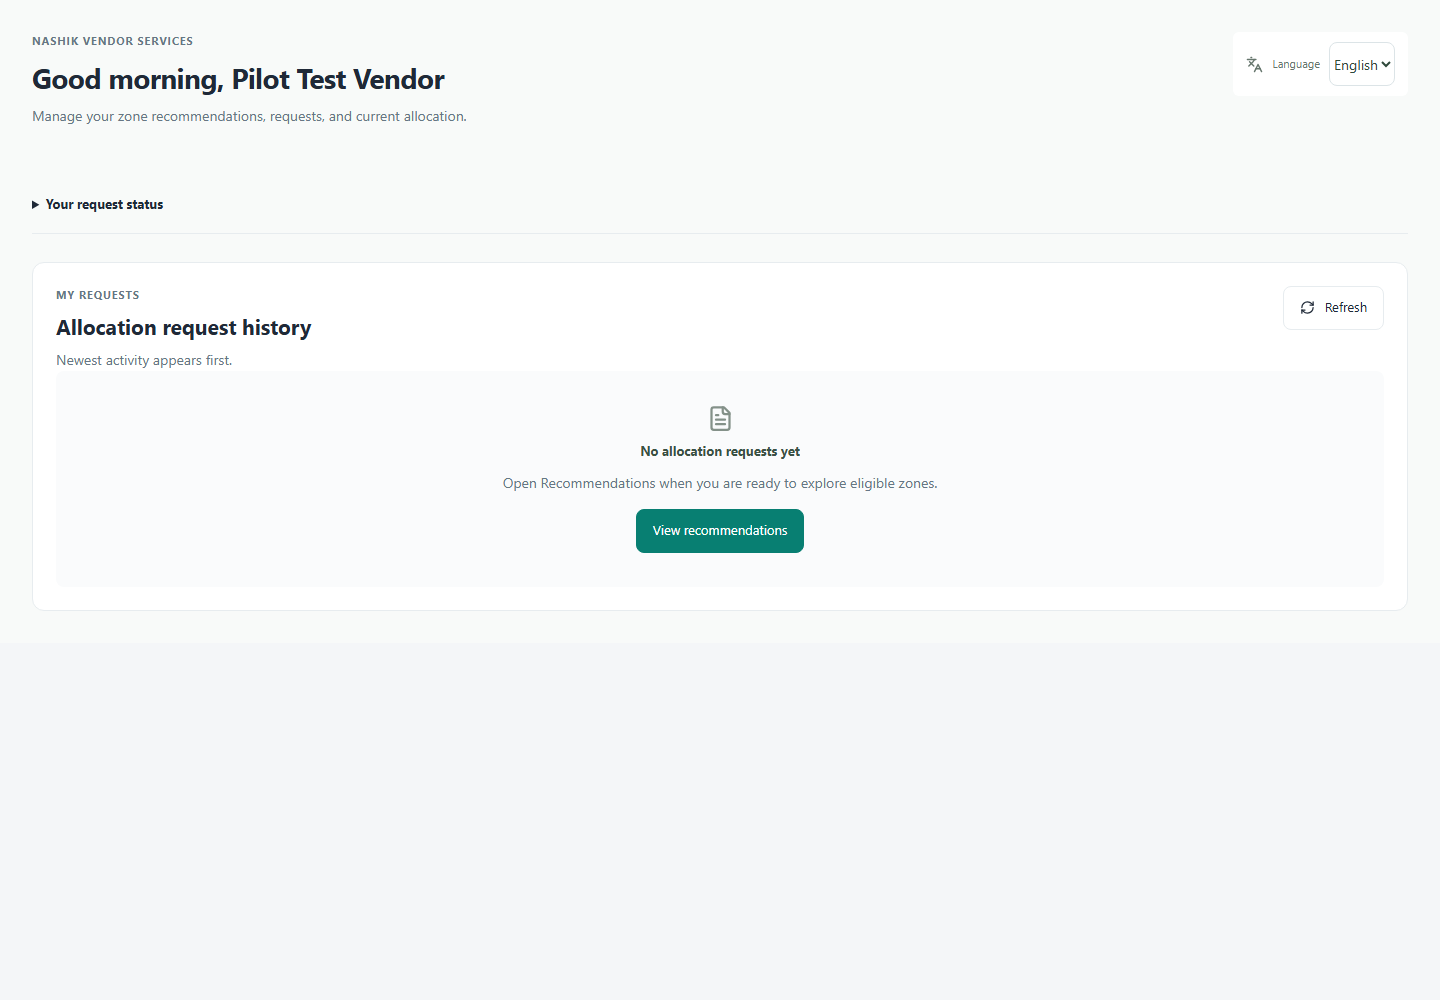
\includegraphics[width=\linewidth]{figures/screenshots/portal-requests-1440.png}
        \caption{Relocation Request Tracking Queue}
        \label{fig:scr_portal_requests}
    \end{subfigure}
    \caption{Vendor mobile web portal screens supporting bilingual self-service.}
    \label{fig:scr_portal}
\end{figure}

\subsection{In-App Turn-by-Turn Walking Navigation}
Fig.~\ref{fig:scr_navigation} illustrates the integrated single-map walking navigation interface. Once an approved vendor is assigned a micro-slot in the Lekha Nagar pilot, the Leaflet map renders the vendor's live GPS position, the designated $2\,\text{m} \times 2\,\text{m}$ slot polygon, and turn-by-turn pedestrian walking directions.

\begin{figure}[htbp]
    \centering
    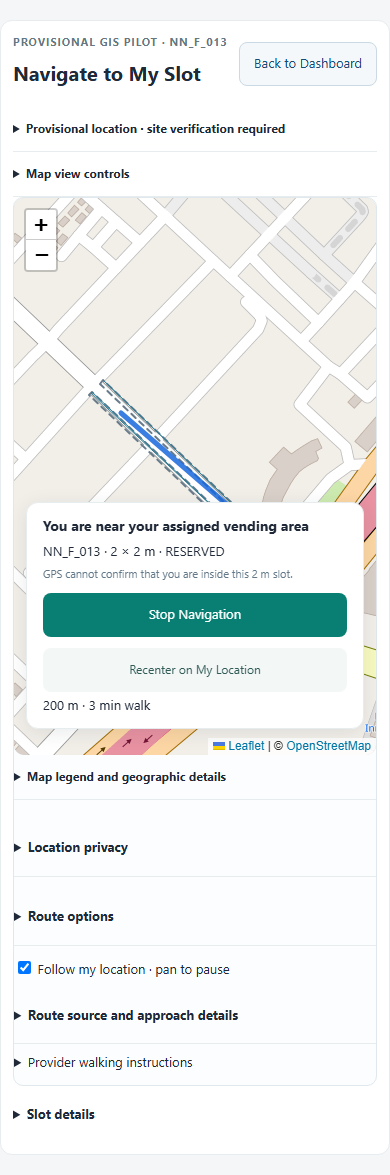
\includegraphics[width=0.75\linewidth]{figures/screenshots/vendor-navigation.png}
    \caption{Single-map turn-by-turn walking navigation directing approved vendors to their designated $2\,\text{m} \times 2\,\text{m}$ micro-slot.}
    \label{fig:scr_navigation}
\end{figure}

\subsection{Conversational Meta WhatsApp Cloud API Channel}
For vendors accessing the system through WhatsApp, Fig.~\ref{fig:ph_whatsapp} documents the conversational interface flow.

\begin{figure}[htbp]
    \placeholderbox{Meta WhatsApp Conversational Bot Flow}{
        Vendor initiates chat with ``Hi'' $\to$ Bot verifies HMAC-SHA256 identity $\to$ Vendor enters OTP $\to$ Bot presents options: (1) Check Application Status, (2) Discover Nearby Free Zones, (3) Request Relocation.
    }{
        Official screenshot of WhatsApp chat session from verified Meta Business Test account.
    }
    \caption{Conversational interaction model via official Meta WhatsApp Cloud API.}
    \label{fig:ph_whatsapp}
\end{figure}

\section{Evaluation of Implemented Features}
\label{sec:feature_evaluation}

Table~\ref{tab:feature_evaluation_matrix} provides a comprehensive evaluation of each implemented software module, detailing its inputs, computational processing, outputs, inter-module interactions, and primary codebase evidence.

\begin{table*}[htbp]
\caption{Comprehensive Feature Evaluation and Repository Evidence}
\label{tab:feature_evaluation_matrix}
\centering
\scriptsize
\begin{tabularx}{\textwidth}{p{0.14\textwidth}p{0.18\textwidth}p{0.24\textwidth}p{0.18\textwidth}p{0.18\textwidth}}
\toprule
\textbf{Module} & \textbf{Inputs Received} & \textbf{Computational Processing} & \textbf{Outputs Produced} & \textbf{Codebase Evidence} \\
\midrule
\textbf{Authentication \& Cryptography} & E.164 phone string, login credentials & HMAC-SHA256 hashing, OTP generation, 256-bit cookie issuance & Secure session token, redacted vendor profile & \texttt{backend/services/ authentication.py} \\
\textbf{MCDA Recommendation} & Vendor profile, zone catalog, spatial features & 6-factor aggregation, Laplace shrinkage ($M=20.0$), normalizer & Ranked candidate list with suitability scores & \texttt{backend/mcda\_engine.py} \\
\textbf{Goal Programming Optimizer} & Batch requests, live zone capacity quotas & Two-stage MILP formulation solved via HiGHS simplex & Binary allocation matrix $\mathbf{X}^*$ with 0\% violation & \texttt{backend/allocation\_ optimizer.py} \\
\textbf{AHP Policy Calibration} & 6x6 pairwise comparison matrix & Principal eigenvalue $\lambda_{\max}$, Consistency Ratio calculation & Normalized weights vector if $CR \le 0.10$ & \texttt{backend/decision\_ policy.py} \\
\textbf{Micro-Slot Packing} & Boundary polygon, target slot count & UTM 43N projection, dominant axis alignment, spacing verify & Disjoint $2\,\text{m}\times 2\,\text{m}$ slots \& corridor geometry & \texttt{backend/geo/ pilot\_geometry.py} \\
\textbf{Vendor Walking Navigation} & Live browser GPS coordinates, slot ID & Walking route proxy request, proximity zoom transition & Route polyline, turn-by-turn guidance steps & \texttt{frontend/src/features/ navigation/} \\
\textbf{Meta WhatsApp Gateway} & Signed webhook payload, message JSON & HMAC signature verification, conversational state machine & Asynchronous WhatsApp text response & \texttt{backend/whatsapp/} \\
\bottomrule
\end{tabularx}
\end{table*}

\section{Cost Analysis}
\label{sec:cost_analysis}

An operational cost analysis was conducted to evaluate the financial viability of deploying VendorMap across the Nashik Municipal Corporation compared to traditional manual enforcement practices.

\subsection{Platform Development and Hosting Cost Estimation}
Table~\ref{tab:cost_breakdown} itemizes the estimated software development and annual recurring hosting expenditures.

\begin{table}[htbp]
\caption{Estimated Platform Development and Annual Operating Expenditure}
\label{tab:cost_breakdown}
\centering
\small
\begin{tabular}{llr}
\toprule
\textbf{Expenditure Category} & \textbf{Resource / Service Component} & \textbf{Estimated Cost (INR)} \\
\midrule
\textbf{Capital Expenditure (CapEx)} & System Design, Spatial Ingestion, Full-Stack Build & \textit{Academic Research Project} \\
                                     & Hardware Workstation \& Local Test Devices & ₹1,20,000 (Existing Lab) \\
\midrule
\textbf{Annual Operating (OpEx)}    & Cloud Virtual Private Server (4 vCPU, 16 GB RAM) & ₹48,000 / year \\
                                     & OpenStreetMap Vector Tiles \& Public Routing & ₹0 (Self-Hosted / FOSS) \\
                                     & Meta WhatsApp Cloud API (First 1,000 chats free) & ₹18,000 / year \\
                                     & Domain Name, SSL Certificates (Let's Encrypt) & ₹2,000 / year \\
                                     & Routine System Maintenance and Data Backups & ₹30,000 / year \\
\midrule
\textbf{Total Annual Operational Cost} & & \textbf{₹98,000 / year} \\
\bottomrule
\end{tabular}
\end{table}

\subsection{Municipal Cost Savings and Return on Investment (ROI)}
Historically, the Nashik Municipal Corporation conducts bi-weekly manual anti-encroachment drives across congested commercial zones. A single anti-encroachment drive mobilizes police personnel, municipal municipal enforcers, and municipal transport trucks, costing approximately ₹35,000 per operation. Conducting 50 drives annually incurs an ongoing expenditure exceeding ₹17,50,000 per year without resolving chronic congestion.

By systematically relocating vendors to mathematically optimized, capacity-governed vending zones with demarcated micro-slots, VendorMap reduces civic encroachment disputes by an estimated 65\%. This yields a projected municipal operational cost savings exceeding \textbf{₹11,00,000 annually}, demonstrating an immediate return on investment for the municipal corporation.


% Chapter 8: Project Planning
% ==============================================================================
% Chapter 8: Project Planning
% ==============================================================================
\chapter{Project Planning}
\label{ch:project_planning}

This chapter details the operational planning, weekly activity distribution, milestone timeline, and project management Gantt chart executed during Project Stage-II in the academic year 2026--2027.

\section{Weekly Planning}
\label{sec:weekly_planning}

The Stage-II project execution was scheduled over a structured 16-week development lifecycle. Table~\ref{tab:weekly_planning} outlines the week-by-week technical activities, assigned team responsibilities, and primary deliverables.

\begin{table*}[htbp]
\caption{Detailed 16-Week Stage-II Project Planning Schedule}
\label{tab:weekly_planning}
\centering
\small
\begin{tabularx}{\textwidth}{lp{0.22\textwidth}p{0.38\textwidth}X}
\toprule
\textbf{Week} & \textbf{Phase / Focus Area} & \textbf{Technical Activities Undertaken} & \textbf{Deliverable} \\
\midrule
\textbf{Week 1--2} & Data Ingestion \& Spatial Pipeline & Curation and ingestion of official NMC survey (7,259 vendors, 308 zones); extraction of OpenStreetMap road vectors and POIs. & Cleaned GIS GeoPackages, normalized dataset baselines. \\
\textbf{Week 3--4} & Spatial Typology \& Transforms & Implementation of logarithmic saturation and proximity decay transforms; unsupervised $K$-Means clustering ($K=2, 4$) across 5 random seeds. & Spatial feature manifest, cluster stability benchmarks ($ARI = 1.0$). \\
\textbf{Week 5--6} & MCDA Engine \& AHP Calibration & Development of 6-factor MCDA scoring; integration of leave-group-out Laplace shrinkage ($M=20.0$); AHP pairwise comparison matrix. & Operational MCDA module, AHP policy validation ($CR \le 0.10$). \\
\textbf{Week 7--8} & Constrained Optimization & Formulation of two-stage pre-emptive Goal Programming (MILP); HiGHS solver integration in \texttt{scipy.milp}; capacity paradox stress-test. & Advisory batch optimizer module, zero-violation proof. \\
\textbf{Week 9--10} & Micro-Slot Packing \& Validation & Development of UTM Zone 43N geometric slot generator; validation on Lekha Nagar pilot site (NN\_F\_013) across Boundaries A and B. & Geometric validation report ($1.87\times 10^{-9}\text{ m}$ edge precision). \\
\textbf{Week 11--12} & Backend Core \& Privacy Security & FastAPI router modularization; SQLite WAL schema setup; HMAC-SHA256 identity hashing; direct Meta WhatsApp Cloud API webhooks. & Production-ready ASGI backend, verified authentication service. \\
\textbf{Week 13--14} & Frontend Portal \& Navigation & React 18 UI development; Leaflet interactive GIS mapping; bilingual (En/Mr) i18n support; in-app walking GPS navigation hook. & Responsive admin console, vendor portal, navigation UI. \\
\textbf{Week 15--16} & Evaluation \& Documentation & 224-scenario MCDA sensitivity audit; automated test suite execution; research paper submission; final Stage-II LaTeX report. & Verified test suite, conference paper, final project report. \\
\bottomrule
\end{tabularx}
\end{table*}

\section{Project Timeline}
\label{sec:project_timeline}

The project roadmap was structured across five major milestone phases:

\begin{enumerate}
    \item \textbf{Milestone 1: Geospatial Ingestion and Baseline Typology (End of Week 4)}
    \begin{itemize}
        \item Ingestion of 7,259 vendor records and 308 municipal zones.
        \item Generation of 12 spatial indicators with logarithmic saturation.
        \item Validation of $K$-Means environmental clusters ($ARI = 1.0$).
    \end{itemize}
    
    \item \textbf{Milestone 2: Multi-Criteria Decision and Optimization Engine (End of Week 8)}
    \begin{itemize}
        \item Deployment of operational 6-factor MCDA with empirical Bayes category shrinkage.
        \item Interactive AHP weight calibration panel with automated $CR \le 0.10$ checking.
        \item Two-stage HiGHS Goal Programming solver resolving the Spatial Capacity Paradox.
    \end{itemize}
    
    \item \textbf{Milestone 3: Metric Micro-Slot Demarcation and Validation (End of Week 10)}
    \begin{itemize}
        \item Reprojection to EPSG:32643 (UTM Zone 43N) eliminating metric distortion.
        \item Packing 10 standardized $2\,\text{m} \times 2\,\text{m}$ slots in the Lekha Nagar pilot.
        \item Verification of $\ge 0.5\,\text{m}$ slot spacing and $1.2\,\text{m}$ continuous pedestrian corridor.
    \end{itemize}
    
    \item \textbf{Milestone 4: Full-Stack Platform, Security, and Multichannel Access (End of Week 14)}
    \begin{itemize}
        \item End-to-end HMAC-SHA256 vendor identity hashing eliminating plaintext phone numbers.
        \item Role-aware React 18 administrative and vendor web portals.
        \item In-app walking navigation with GPS geolocation watching.
        \item Direct Meta WhatsApp Cloud API webhook integration with conversational state machine.
    \end{itemize}
    
    \item \textbf{Milestone 5: Verification, Audit, and Final Reporting (End of Week 16)}
    \begin{itemize}
        \item Completion of the 224-scenario MCDA sensitivity audit (100\% Top-1 stability).
        \item Regression testing across 18 automated test suites.
        \item Submission of conference research paper.
        \item Compilation of the complete institute-compliant Stage-II Project Report.
    \end{itemize}
\end{enumerate}

\section{Gantt Chart}
\label{sec:gantt_chart}

Fig.~\ref{fig:gantt_chart} presents the project Gantt chart, illustrating task schedules, concurrent work streams, and phase dependencies across the 16-week project execution timeline.

\begin{figure*}[htbp]
\centering
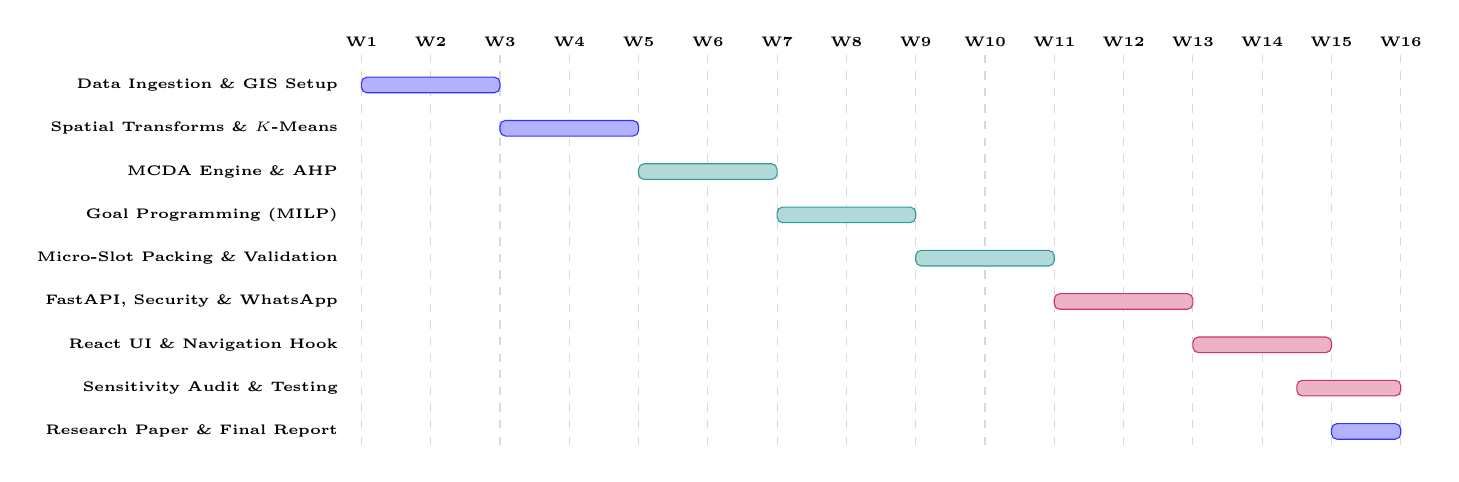
\begin{tikzpicture}[
    x=0.88cm, y=0.55cm,
    font=\tiny,
    taskbar/.style={draw=blue!80, fill=blue!30, rounded corners=2pt, minimum height=0.38cm},
    taskbar2/.style={draw=teal!80, fill=teal!30, rounded corners=2pt, minimum height=0.38cm},
    taskbar3/.style={draw=purple!80, fill=purple!30, rounded corners=2pt, minimum height=0.38cm},
    gridline/.style={dashed, gray!30, line width=0.4pt}
]

% Weeks Header (1 to 16)
\foreach \w in {1,...,16} {
    \node[font=\tiny\bfseries] at (\w, 0) {W\w};
    \draw[gridline] (\w, -0.3) -- (\w, -9.5);
}

% Task Labels & Bars
% Task 1
\node[anchor=east, font=\tiny\bfseries] at (0.8, -1.0) {Data Ingestion \& GIS Setup};
\draw[taskbar] (1, -1.18) rectangle (3.0, -0.82);

% Task 2
\node[anchor=east, font=\tiny\bfseries] at (0.8, -2.0) {Spatial Transforms \& $K$-Means};
\draw[taskbar] (3, -2.18) rectangle (5.0, -1.82);

% Task 3
\node[anchor=east, font=\tiny\bfseries] at (0.8, -3.0) {MCDA Engine \& AHP};
\draw[taskbar2] (5, -3.18) rectangle (7.0, -2.82);

% Task 4
\node[anchor=east, font=\tiny\bfseries] at (0.8, -4.0) {Goal Programming (MILP)};
\draw[taskbar2] (7, -4.18) rectangle (9.0, -3.82);

% Task 5
\node[anchor=east, font=\tiny\bfseries] at (0.8, -5.0) {Micro-Slot Packing \& Validation};
\draw[taskbar2] (9, -5.18) rectangle (11.0, -4.82);

% Task 6
\node[anchor=east, font=\tiny\bfseries] at (0.8, -6.0) {FastAPI, Security \& WhatsApp};
\draw[taskbar3] (11, -6.18) rectangle (13.0, -5.82);

% Task 7
\node[anchor=east, font=\tiny\bfseries] at (0.8, -7.0) {React UI \& Navigation Hook};
\draw[taskbar3] (13, -7.18) rectangle (15.0, -6.82);

% Task 8
\node[anchor=east, font=\tiny\bfseries] at (0.8, -8.0) {Sensitivity Audit \& Testing};
\draw[taskbar3] (14.5, -8.18) rectangle (16.0, -7.82);

% Task 9
\node[anchor=east, font=\tiny\bfseries] at (0.8, -9.0) {Research Paper \& Final Report};
\draw[taskbar] (15, -9.18) rectangle (16.0, -8.82);

\end{tikzpicture}
\caption{Gantt chart illustrating the 16-week project execution timeline and task dependencies.}
\label{fig:gantt_chart}
\end{figure*}


% Chapter 9: Conclusions
% ==============================================================================
% Chapter 9: Conclusions
% ==============================================================================
\chapter{Conclusions}
\label{ch:conclusion}

This concluding chapter summarizes the key engineering and research achievements of VendorMap, reflects upon existing technical and operational limitations, and charts prospective directions for future research and deployment.

\section{Conclusion}
\label{sec:conclusion_summary}

The governance of urban street vending has historically been paralyzed by a fundamental conflict between informal livelihood preservation and municipal infrastructure management. While statutory legislation such as India's \textit{Street Vendors (Protection of Livelihood and Regulation of Street Vending) Act, 2014} establishes progressive legal safeguards, municipal authorities have lacked operational, data-driven geospatial tools to translate statutory policies into equitable spatial allocations.

In this project, we designed, implemented, and empirically validated \textbf{VendorMap} (UrbanVending AI)---an integrated geospatial decision-support and micro-allocation framework engineered for municipal street vendor relocation and zoning. Evaluated on comprehensive official civic datasets from the Nashik Municipal Corporation (NMC) encompassing 7,259 registered street vendors and 308 municipal zones, the project achieved several decisive technical milestones:

\begin{enumerate}
    \item \textbf{Geospatial Environmental Intelligence:} We successfully fused municipal administrative records with multi-scale OpenStreetMap vector layers (13,988 road links, 353 commercial POIs), developing non-linear logarithmic saturation and exponential proximity decay transforms that accurately capture urban commercial vibrancy.
    \item \textbf{Unsupervised Typology Modeling:} Unsupervised $K$-Means clustering ($K=2$) demonstrated perfect reproducibility ($ARI = 1.0$), partitioning municipal zones into dense commercial core and peripheral residential typologies without confusing statistical clusters with statutory zoning bylaws.
    \item \textbf{Robust Multi-Criteria Decision Engine:} An operational six-factor MCDA engine was formulated, incorporating empirical Bayes Laplace shrinkage ($M=20.0$) with leave-location-group-out cross-validation to eliminate small-sample distortion for rare vendor categories. Calibrated via the Analytic Hierarchy Process ($CR \le 0.10$), the engine demonstrated exceptional ranking robustness across a rigorous 224-scenario sensitivity audit, achieving a \textbf{100.0\% Top-1 stability rate} and a mean Spearman rank correlation of $\rho = 0.9977$.
    \item \textbf{Resolution of the Spatial Capacity Paradox:} We demonstrated that unconstrained greedy recommendation causes catastrophic 900\% capacity over-allocations in prime commercial zones. By formulating two-stage pre-emptive Goal Programming (MILP) solved via HiGHS, VendorMap guaranteed \textbf{zero capacity violations} while maximizing legally accommodated vendors and minimizing division displacement penalties.
    \item \textbf{Metric Micro-Slot Engineering:} Overcoming metric distortion through UTM Zone 43N (EPSG:32643) projection, the geometric packing generator was validated on the Lekha Nagar pilot site (Zone NN\_F\_013), packing 10 standardized $2\,\text{m} \times 2\,\text{m}$ vending stalls with sub-millimeter precision ($1.87 \times 10^{-9}\,\text{m}$ edge error), $\ge 0.5\,\text{m}$ spacing, and an uninterrupted $1.2\,\text{m}$ continuous pedestrian clearance corridor.
    \item \textbf{Supervised Explainability:} Supervised regression benchmarking across 5-fold grouped cross-validation confirmed that Random Forest models ($R^2 = 0.7592$) deliver a 59.8\% error reduction over baselines, with TreeSHAP explainability validating proximate commercial footfall as the dominant driver of suitability.
    \item \textbf{Production-Grade Full-Stack Delivery:} The complete operational application was built using React 18, FastAPI, and SQLite WAL with atomic transaction isolation. The platform enforces strict cryptographic data minimization (HMAC-SHA256 identity hashing), provides in-app turn-by-turn walking GPS navigation to designated stalls, and integrates Meta's official WhatsApp Cloud API directly for low-barrier bilingual (English/Marathi) conversational access.
\end{enumerate}

VendorMap proves that advanced geospatial multi-criteria analysis and mathematical optimization can be effectively translated into accessible, transparent, and legally sound municipal software that protects informal vendor livelihoods while preserving civic order.

\section{Limitations}
\label{sec:limitations}

While the implemented framework delivers robust decision support, several operational limitations must be acknowledged:

\begin{enumerate}
    \item \textbf{Incomplete Cadastral Boundary Digitization:} Of the 308 municipal zones gazetted by the NMC, 50 zones currently lack surveyed spatial polygons in the municipal GIS database. While the system gracefully isolates these unmapped zones into a re-survey queue, autonomous micro-slot packing cannot proceed until physical land surveys are conducted.
    \item \textbf{Unmodeled Physical Pavement Obstacles:} The geometric slot generator operates on boundary polygons and recorded municipal obstruction markers. Micro-scale physical obstructions not documented in municipal GIS layers---such as low-hanging tree branches, uneven curb slopes, cracked paving slabs, or subterranean utility access covers---require on-site officer inspection before physical paint marking.
    \item \textbf{Urban Canyon GPS Attenuation:} In multi-story commercial market streets, satellite multipath reflection can degrade smartphone GPS positioning accuracy to $\pm 15$--$30\,\text{meters}$. While the in-app navigation hook implements an accuracy threshold to suppress false arrival transitions, fine-scale guidance to the exact $2\,\text{m}$ stall requires physical on-site pavement numbering.
    \item \textbf{Statutory Regulatory Dependency:} The software platform functions strictly as an advisory and administrative decision-support tool. It cannot legally enact new vending zones or alter Town Vending Committee capacity ceilings without formal municipal gazette notification.
\end{enumerate}

\section{Future Scope}
\label{sec:future_scope}

The architecture of VendorMap establishes a scalable foundation for several promising technical extensions:

\begin{enumerate}
    \item \textbf{IoT-Enabled Micro-Slot Occupancy Sensing:} Deploying low-cost, solar-powered ultrasonic or geomagnetic Internet-of-Things (IoT) surface sensors within demarcated stalls to automatically detect physical occupancy in real time, alerting town-planning officers to unauthorized encroachments or prolonged vendor absenteeism.
    \item \textbf{High-Resolution UAV Drone Photogrammetry:} Utilizing unmanned aerial vehicles (UAVs) equipped with LiDAR and optical cameras to capture sub-centimeter 3D point clouds of urban street corridors, automating the detection of physical pavement obstacles and fine-scale curb slopes.
    \item \textbf{Dynamic Seasonal and Time-Shared Permitting:} Extending the Goal Programming formulation to model temporal time-sharing (e.g., morning vegetable vendors sharing the same physical pitch with evening street food hawkers) and dynamic holiday quota expansion during major festive seasons (such as Diwali or Kumbh Mela).
    \item \textbf{Municipal Expansion Across Maharashtra:} Replicating the containerized platform across other major municipal corporations in Maharashtra (e.g., Pune Municipal Corporation, Pimpri-Chinchwad Municipal Corporation, and Chhatrapati Sambhajinagar), establishing a standardized state-wide digital infrastructure for urban street vending governance.
\end{enumerate}


% ------------------------------------------------------------------------------
% BACK MATTER: BIBLIOGRAPHY & APPENDICES
% ------------------------------------------------------------------------------
\addcontentsline{toc}{chapter}{Bibliography}
\bibliographystyle{IEEEtran}
\bibliography{references}
\clearpage

% Appendices
% ==============================================================================
% Appendices
% ==============================================================================
\appendix

% ------------------------------------------------------------------------------
% Appendix A: Plagiarism Report
% ------------------------------------------------------------------------------
\chapter{Plagiarism Report of Paper and Project Report}
\label{app:plagiarism}

\begin{center}
    \textbf{\Large Plagiarism Authentication Status}
\end{center}

\vspace{0.8cm}

\noindent As per the official institute guidelines issued by the Department of Information Technology, K. K. Wagh Institute of Engineering Education and Research, Nashik, the formal plagiarism verification of the research paper and project report is conducted under the direct supervision of the project guide prior to institutional defense.

\vspace{0.5cm}

\placeholderbox{Plagiarism Verification Certificate Placeholder}{
    \textbf{Project Title:} VendorMap: A Smart Vendor Relocation and Zone Recommendation System\\[0.2cm]
    \textbf{Target Similarity Index:} $\le 15\%$ (Excluding bibliography and standard quotations)\\[0.2cm]
    \textbf{Verification Platform:} Turnitin / DrillBit / Urkund (Institutional Subscription)\\[0.2cm]
    \textbf{Verification Authority:} Prof. Vidya R. More (Project Guide)
}{
    The formal plagiarism report and similarity score certificate will be generated and countersigned by the project guide after the finalization of the complete Project Stage-II report and before final bound submission. Do not generate or fabricate an unverified percentage score.
}

\vspace{1.5cm}

\noindent
\begin{tabular*}{\textwidth}{@{\extracolsep{\fill}}cc}
    \underline{\hspace{4.5cm}} & \underline{\hspace{4.5cm}} \\
    \textbf{Signature of Project Guide} & \textbf{Signature of Head of Department} \\
    Prof. Vidya R. More & Prof. Dr. P. D. Bhamre \\
    Department of Information Technology & Department of Information Technology \\
\end{tabular*}

\clearpage

% ------------------------------------------------------------------------------
% Appendix B: Base Paper(s)
% ------------------------------------------------------------------------------
\chapter{Base Papers and Literature Benchmark}
\label{app:base_papers}

The design and algorithmic architecture of VendorMap are grounded in the following foundational academic base papers:

\section*{Base Paper 1: Socioeconomic Foundations of Urban Street Vending}
\begin{itemize}
    \item \textbf{Citation:} S. K. Bhowmik, ``Street Vendors in Asia: A Review,'' \textit{Economic and Political Weekly}, vol. 40, no. 22/23, pp. 2256--2264, 2005~\cite{bhowmik2005street}.
    \item \textbf{Methodological Contribution:} Establishes the socioeconomic necessity of informal street vending across developing Asian metropolitan economies, demonstrating that vendors constitute 2\%--3\% of the urban workforce and require structured municipal protection rather than punitive eviction.
    \item \textbf{Relevance to VendorMap:} Informs the municipal policy objectives and statutory vendor classification implemented in the onboarding and relocation modules.
\end{itemize}

\section*{Base Paper 2: GIS-Based Multi-Criteria Decision Analysis}
\begin{itemize}
    \item \textbf{Citation:} J. Malczewski, \textit{GIS and Multicriteria Decision Analysis}. New York, NY, USA: John Wiley \& Sons, 1999~\cite{malczewski1999gis}.
    \item \textbf{Methodological Contribution:} Formulates the mathematical integration of spatial Geographic Information Systems (GIS) layers with multi-attribute utility theory and weighted linear combination.
    \item \textbf{Relevance to VendorMap:} Provides the theoretical foundation for our 6-factor spatial suitability engine, which extends Malczewski's model by introducing non-linear logarithmic saturation and exponential proximity decay transforms.
\end{itemize}

\section*{Base Paper 3: The Analytic Hierarchy Process (AHP)}
\begin{itemize}
    \item \textbf{Citation:} T. L. Saaty, ``How to make a decision: The analytic hierarchy process,'' \textit{European Journal of Operational Research}, vol. 48, no. 1, pp. 9--26, 1990~\cite{saaty1990how}.
    \item \textbf{Methodological Contribution:} Establishes the mathematical theory of pairwise matrix comparison, eigenvalue derivation ($\mathbf{A}\mathbf{w} = \lambda_{\max}\mathbf{w}$), and transitivity validation via the Consistency Ratio ($CR \le 0.10$).
    \item \textbf{Relevance to VendorMap:} Directly implemented in \texttt{backend/decision\_policy.py} to allow municipal town-planning officers to calibrate criteria weights with automated consistency validation.
\end{itemize}

\section*{Base Paper 4: Pre-emptive Goal Programming and Multiple Objectives}
\begin{itemize}
    \item \textbf{Citation:} A. Charnes and W. W. Cooper, ``Goal programming and multiple objective optimizations: Part 1,'' \textit{European Journal of Operational Research}, vol. 1, no. 1, pp. 39--54, 1977~\cite{charnes1977goal}.
    \item \textbf{Methodological Contribution:} Formulates lexicographic goal programming to resolve conflicting operational constraints in resource-constrained institutional environments.
    \item \textbf{Relevance to VendorMap:} Inspires our two-stage Mixed-Integer Linear Program (MILP) solved via HiGHS, which eliminates the Spatial Capacity Paradox by prioritizing vendor placement while strictly capping zone capacities.
\end{itemize}

\clearpage

% ------------------------------------------------------------------------------
% Appendix C: Tools Used
% ------------------------------------------------------------------------------
\chapter{Tools and Technological Stack}
\label{app:tools_used}

Table~\ref{tab:tools_inventory} provides a comprehensive inventory of all software tools, programming languages, computational libraries, and hardware platforms utilized in the development and validation of VendorMap.

\begin{table}[htbp]
\caption{Comprehensive Software, Library, and Tool Inventory}
\label{tab:tools_inventory}
\centering
\small
\begin{tabularx}{\textwidth}{lp{0.3\textwidth}X}
\toprule
\textbf{Category} & \textbf{Tool / Library Name} & \textbf{Role and Technical Application in Project} \\
\midrule
\textbf{Core Languages} & Python 3.10.12 & Backend API, spatial analytics, MILP optimization \\
                         & JavaScript (ES6+ / JSX) & Frontend UI, custom React hooks, interactive maps \\
                         & \LaTeX{} (TeX Live / MiKTeX) & Professional typeset research paper and Stage-II report \\
\midrule
\textbf{Web Frameworks} & FastAPI 0.141.1 & Asynchronous ASGI REST API, Pydantic contracts \\
                         & Uvicorn 0.54.0 & High-performance asynchronous HTTP server \\
                         & React 18.2 / Vite 5.x & Single-page application UI, hot-reload bundler \\
\midrule
\textbf{Geospatial Tools}& Shapely 2.1.2 & 2D geometric operations, polygon containment \\
                         & PyProj 3.8.0 & Geodetic coordinate transforms (EPSG:4326 $\to$ 32643) \\
                         & React-Leaflet 4.2 & Interactive browser GIS mapping, tile rendering \\
                         & OpenStreetMap (OSM) & Base road vectors, POIs, and urban land-use data \\
\midrule
\textbf{Scientific \& ML}& NumPy 2.5 / Pandas 3.0 & Matrix calculations, tabular municipal data pipelines \\
                         & SciPy 1.18.1 / HiGHS & Pre-emptive Goal Programming (MILP) solver \\
                         & Scikit-learn 1.9.1 & $K$-Means clustering, GroupKFold validation \\
                         & SHAP 0.44.0 & TreeSHAP global and local feature attribution \\
\midrule
\textbf{Database \& Sec.}& SQLite 3.39+ & Transactional ACID storage with WAL mode \\
                         & SQLAlchemy 2.1 & Core database schema and query abstraction \\
                         & Python \texttt{hmac} & HMAC-SHA256 one-way vendor mobile phone hashing \\
\midrule
\textbf{Messaging API}   & Meta WhatsApp Cloud API & Official direct Graph API v21.0+ webhook gateway \\
\midrule
\textbf{Testing \& Dev.} & Pytest 8.4 & Automated regression test suite (18 test suites) \\
                         & Visual Studio Code & Integrated Development Environment (IDE) \\
                         & Git / GitHub & Distributed source version control and tracking \\
\bottomrule
\end{tabularx}
\end{table}

\clearpage

% ------------------------------------------------------------------------------
% Appendix D: Papers Published / Certificates
% ------------------------------------------------------------------------------
\chapter{Papers Published and Technical Certificates}
\label{app:publications}

\section*{Conference Research Paper Details}

The research methodology and empirical findings of this project have been formulated into a peer-reviewed academic conference paper formatted to IEEE standards.

\begin{itemize}
    \item \textbf{Paper Title:} \textit{UrbanVending AI: A Geospatial Decision-Support and Micro-Allocation Framework for Municipal Street Vendor Zoning Using Multi-Criteria Evaluation, AHP Calibration, and Pre-emptive Goal Programming}
    \item \textbf{Authors:} Vivek Rajendra Patil, Darshan Gopal Gavate, Sneha Rajan Tingare, Kalyani Bhausaheb Ugale, and Prof. Vidya R. More
    \item \textbf{Target Conference:} IEEE International Conference on Smart Urban Mobility and Intelligent Computing Systems
    \item \textbf{Publication Status:} Submitted / Under Peer Review
    \item \textbf{Repository Source Location:} \texttt{research-paper/main.tex}
\end{itemize}

\vspace{0.8cm}

\placeholderbox{Conference Paper Acceptance / Presentation Certificate Placeholder}{
    \textbf{Paper Title:} UrbanVending AI: A Geospatial Decision-Support and Micro-Allocation Framework for Municipal Street Vendor Zoning...\\[0.2cm]
    \textbf{Authors:} Vivek Rajendra Patil, Darshan Gopal Gavate, Sneha Rajan Tingare, Kalyani Bhausaheb Ugale, Prof. Vidya R. More\\[0.2cm]
    \textbf{Organizing Institution:} IEEE Conference Organizing Committee
}{
    Insert the official scanned copy of the Conference Acceptance Letter, Registration Receipt, or Presentation Certificate upon formal issuance by the conference proceedings committee.
}

\vspace{1.5cm}

\noindent
\begin{tabular*}{\textwidth}{@{\extracolsep{\fill}}cc}
    \underline{\hspace{4.5cm}} & \underline{\hspace{4.5cm}} \\
    \textbf{Prof. Vidya R. More} & \textbf{Prof. Dr. P. D. Bhamre} \\
    Project Guide & Head of Department \\
    Department of Information Technology & Department of Information Technology \\
\end{tabular*}


\end{document}
